\chapter{Модификация двойного каскада для обогащения регенерированного урана в условиях многократного рецикла}\label{ch:ch3}

Некоторые из рассмотренных в предыдущих главах каскадных схем, частично или полностью позволяют решить проблемы, связанные с присутствием в урановой смеси изотопов $^{232,233,234}$U только для составов регенерированного урана с относительно низким содержанием четных изотопов и исходным содержанием $^{232}$U ниже, чем предельные значения для товарного НОУ. Однако при использовании таких схем для возврата состава загрязненного регенерированного урана, прошедшего несколько циклов использования в качестве топлива легководных реакторов, как правило, уже не удается полностью решить задачу его обогащения, выполнив одновременно весь набор ограничений.

Отсюда и возникает потребность в разработке каскадных схем, которые в состоянии полностью решить задачу обогащения регенерата, не только обеспечив выполнение требований по содержанию четных изотопов в продукте, но и выполнив поставленные требования по расходованию 100\%-ов имеющегося в распоряжении регенерированного урана. Второе условие позволяет вернуть в топливный цикл весь выделенный из ОЯТ регенерат вне зависимости от его изотопного состава, что гарантирует возможность использования подобной схемы для обогащения регенерата урана при его многократном рецикле.

\section{Разработка каскадной схемы для обогащения регенерированного урана с одновременным выполнением условия на отношение используемого регенерата по отношению к производимому продукту, а также ограничений на концентрации четных изотопов}
\subsection{Описание предлагаемой схемы}\label{triple_descr}

Основной проблемой, подлежащей решению в настоящей работе, является поиск варианта каскадной схемы, позволяющей одновременно выполнить условия по четным изотопам и задействовать в обогащении весь поступивший регенерат при различных внешних условиях и различных исходных составах регенерата.

Невозможность возврата регенерата в производство топлива с использованием многочисленных модификаций каскада для обогащения многократно облученного регенерата, во многом, связана с ростом величин относительных концентраций «легких» изотопов (в первую очередь $^{232}$U) по отношению к $^{235}$U в поступающем в обогащении регенерате. Далее, в процессе обогащения относительные концентрации легких изотопов по отношению к $^{235}$U также возрастают. Это связано с тем, что при обогащении $^{235}$U более легкие изотопы концентрируются вместе с ним. При использовании схем на основе одиночного ординарного каскада единственным способом понизить относительную концентрацию изотопов  $^{232}$U и $^{235}$U является разбавление смеси обогащаемого регенерата материалом, не содержащим $^{232}$U, например на входе в каскад \cite{smirnovKaskadnyeShemyZadachah2012}. Однако, результаты вычислительных экспериментов, проведенных для различных разбавителей показывают, что для составов с высоким исходным содержанием $^{232}$U (выше предельных значений для товарного НОУ) невозможно подобрать разбавитель такой, чтобы удовлетворить одновременно условия полного возврата регенерата в цикл и заданные ограничения на концентрации четных изотопов в товарном продукте (см. Главу \ref{ch:ch2}). 

Решение данной проблемы может быть основано на использовании двойных каскадов, позволяющих частично отделить друг от друга изотопы $^{232}$U и $^{235}$U, что позволяет выполнить ограничения на концентрации четных изотопов в товарном НОУ без разбавления регенерата сырьем, не содержащим $^{232}$U и $^{236}$U. Однако, как показано в Главе 3 простой вариант двойного каскада также не позволяет решить задачу. 

Предлагаемый вариант каскадной схемы состот из двух подсистем (рис. \ref{p2left}): первая представляет собой двойной каскад (каскады I и II на рис. \ref{p2left}), вторая представляет собой ординарный каскад для обогащения природного урана (каскад III на рис. \ref{p2left}). В первом каскаде подсистемы I обогащают исходный регенерат изотопами $^{232,233,234,235,236}$U. В каскаде II смесь делится на две фракции, так, чтобы в потоке тяжелой фракции ($W_2$) было понижено содержание $^{232,233,234}$U по отношению к питающей второй каскад смеси -- потоку $P_1$. 

\begin{figure}[ht]
    \centerfloat{
\includegraphics[scale=0.9]{cascades/p2left}}
    \caption{Схема модифицированного двойного каскада для обогащения регенерированного урана. Обозначения: $E$ -- поток регенерированного урана; $P_1$ -- поток отбора первого каскада, выступающий питанием второго каскада; $P_2$ -- поток отбора второго каскада; $W_1$ -- поток отвала первого каскада; $W_2$ -- поток тяжелой фракции (условный «отвал») второго каскада; $P_0$ -- поток НОУ-разбавителя; $P$ -- финальный продукт (товарный низкообогащенный уран (НОУ))}\label{p2left}
\end{figure}

является развитием идеи, впервые предложенной в работе \cite{vodolazskihSposobIzotopnogoVosstanovleniya2006}.

Концентрация $^{235}$U в потоке $P_1$ должна быть больше концентрации $^{235}$U в конечном продукте, ввиду того, что во втором каскаде получаемый продукт будет обедняться по $^{235}$U. Что касается верхней границы концентрации ${C}_{235,{P_1}}$, то она с физической точки зрения может быть ограничена только предельно достижимой концентрацией $^{235}$U в этом потоке, определяемой по известным соотношениям \cite{sulaberidzeOsobennostiObogashcheniyaKomponentov2006}, \cite{minenkoPredelnoeObogashcheniePromezhutochnyh1972}. С другой стороны при задании параметров каскадов подсистемы I необходимо согласовывать значения концентраций ${C}_{235,{P_1}}$ и ${C}_{235,{P_2}}$, поскольку должно выполняться очевидное соотношение ${C}_{235,{P_2}}{>}{C}_{235,{P_1}}$.
% Далее, полученный в первом каскаде обогащенный уран направляется на вход второго каскада, где он разделяется на 2 группы: в первой концентрируются легкие изотопы и $^{235}$U, во второй легкие изотопы обедняются, параллельно с относительно небольшим снижением концентрации $^{235}$U.
Выбор $C_{235,{P_2}}$ может определяться не только физическими соображениями, но и формальными. Учитывая, что поток $P_2$ является одним из внешних, выходящих из схемы рис. \ref{p2left} потоков, то на него могут распространяться, например, требования о непревышение порога обогащения в 20\%. Такое ограничение обусловлено тем, что уран, обогащенный до 20\% и выше, по критериям МАГАТЭ считают материалом прямого использования, т.е. пригодным для создания ядерно-взрывных устройств \cite{brownOriginsSignificanceLimit2016}, \cite{pshakinYadernoeNerasprostranenie2006}. Превышение данного порога может оказаться критичным с формальной с точки зрения нормативных документов, однако данное ограничение не является физическим, что позволяет потенциально рассматривать и значения концентраций  $C_{235,{P_2}}$ выше этой величины. 

Финальным шагом к получению конечного НОУ-продукта является разбавление потока $W_2$ второго каскада сырьем, не содержащим искусственных изотопов урана для выполнения ограничений по $^{232}$U и $^{236}$U.
Для этого используют вторую подсистему (каскад III), предназначенную для наработки разбавителя заданной массы и заданного обогащения по $^{235}$U.
Необходимо учесть то, что при заданных концентрациях $^{235}$U в потоках ${P_1}, {W_1}, {P_2}, {W_2}$ и отношении потоков $E/P$, отношение потоков ${W_2}{/P}$ также будет заданным, что подтверждает приведенное ниже выражение:

\begin{equation}
    \label{dc1}
    \frac{W_{2}}{P}=\frac{P_{1}}{E}\cdot\frac{W_{2}}{P_{1}}\cdot\frac{E}{P}
  \end{equation}


, где $E$ -- поток исходного регенерата, а $P$ -- поток конечного продукта НОУ-продукта.

В дополнение к \ref{dc1} запишем очевидное равенство:

\begin{equation}
    \label{dc2}
    \frac{P_{0}}{P} = 1 - \frac{W_{2}}{P}
\end{equation}

Из \ref{dc1} и \ref{dc2} следует, что отношение потоков ${W_2}{/}{P_0}$ также будет заданным. Иными словами, соотношение между потоками $W_2$ и $P_0$ при их смешивании зависит от выбора параметров каскадов подсистемы I. В этом случае единственным параметром, влияющим на концентрацию $^{235}$U в товарном НОУ является концентрация данного изотопа в разбавителе (поток $P_0$ на схеме рис. \ref{p2left}), которая связана с остальными параметрами соотношением, выражающим закон сохранения вещества для узла смешивания потоков $W_2$ и $P_0$: 

\begin{equation}
    \label{dc3}
    C_{235,P_{0}}=C_{235,P}({1 + \frac{W_{2}}{P_{0}}}) - \frac{W_{2}}{P_{0}}\cdot C_{235,W_{2}}
\end{equation}


Фактически подмешивание НОУ-разбавителя призвано добиться выполнения требуемых условий на концентрации четных изотопов, а также достижения заданного отношения $E{/}P$.

Принимая во внимание очевидные неравенства для потоков в каскадах I и II каскадной схемы:

\begin{equation}
    \label{dc3a}
    W_{2} < P_{1} <  E
\end{equation}

а также характерный диапазон изменения величины потока $E$ в сравнении с потоком $P$:
\begin{equation}
    \label{dc3b}
    E = {(}0,90-0,97{)}P
\end{equation}

можно легко увидеть, что величина потока $W_{2}$ будет в несколько раз меньше, чем величина потока E, и, соответственно, конечного продукта в виде потока P. Следовательно, поток разбавителя $P_{0}$ должен в несколько раз превосходить по величине поток $W_{2}$. 

Таким образом, при заданных концентрациях $^{235}$U в выходящих потоках каскадов I и II, для рассматриваемой схемы единственным параметром, позволяющим корректировать концентрацию в $^{235}$U в потоке P является концентрация данного изотопа в $P_{0}$. Однако, если в качестве разбавителя использовать, например, природный уран, может оказаться невозможным достижение требуемой концентрации $^{235}$U в потоке P. Причиной этому является фиксированность концентрации $^{235}$U таком разбавителе. В этой связи целесообразно, в качестве разбавителя использовать низкообогащенный уран, величина конкретного обогащения которого должна быть определена на основе расчета для каждого входящего состава регенерата и для каждого набора параметров каскадов I и II. В качестве сырья $F_0$ для наработки такого разбавителя, наряду с природным ураном, может быть использован и складской обедненный уран, нарабатывавшийся в ходе производства обогащенного урана из природного урана. При этом такой разбавитель получают обогащением выбранного сырья в отдельном каскаде (каскад III).
% Выбор ОГФУ в качестве сырья НОУ-разбавителя позволяет не расходовать природный уран в процессе рециклирования топлива, ценой дополнительных затрат разделительной работы, что может оказаться привлекательной возможностью в некоторых случаях, особенно при росте цены на природный уран.

Подытоживая выше сказанное, отметим, что каскады I и II в данной схеме работают только с регенерированным ураном, позволяя частично отделить $^{235}$U от более легких $^{232}$U и $^{234}$U. Роль каскада III состоит в наработке разбавителя $P_{0}$, необходимого для формирования требуемой массы конечного продукта с одновременным выполнением условий по четным изотопам в этом продукте. Заметим также, что каскад, нарабатывающий НОУ-разбавитель $P_{0}$, вообще говоря, не является неотъемлемой частью каскадной схемы. При практической реализации подобного подхода каскад для наработки разбавителя может быть обособленным и физически не связанным с каскадами, обогащающими регенерированный уран. Это означает, что разделительные мощности, связанные с обогащением регенерата в такой схеме полностью отделены от разделительных мощностей, работающих с природным ураном. В этом случае исключено загрязнение чётными изотопами разделительного оборудования, работающего с природным ураном. Кроме того, с технической точки зрения обособленность каскадов для обогащения регенерата позволяет при необходимости реализовать на таком производстве дополнительные меры радиационной и физической защиты, учитывая необходимость получать относительно высокие концентрации изотопа $^{235}$U и чётных изотопов, не затрагивая штатное производство по обогащению природного урана.

% Величина потока разбавителя $P_0$, как показывают предварительные оценки параметров каскадной схемы необходимых для получения НОУ-продукта требуемых качеств,  должна в несколько раз превосходить по величине поток тяжелой фракции второго каскада $W_2$. Если бы в качестве разбавителя использовали природный уран, это бы привело к снижению концентрации $^{235}$U в результирующей смеси ниже требуемой величины. Именно поэтому в схеме предусмотрен дополнительный каскад, нарабатывающий низкообогащенный уран в потоке $P_0$ из смесей природного (нереакторного) происхождения -- природного или обедненного урана.

\subsection{Анализ постановок задач и методика расчета каскадной схемы}\label{statement}

В настоящем подразделе описана предложенная в работе методика расчёта предлагаемой схемы обогащения регененированного урана в условиях его многократного рецикла. В качестве модели для описания массопереноса в каскаде для разделения многокомпонентных смесей использован <<квазиидеальный>> каскад \cite{sazykinKvaziidealnyeKaskadyDlya2000}. 

Задача моделирования обогащения регенерированного урана в каскадной схеме рис. \ref{p2left} может быть сформулирована следующим образом.
Задано:

\begin{itemize}
    \item концентрации компонентов в обогащаемом регенерированном уране -- $C_{i,{E}}$; 
    \item отношение потоков $E/P$ -- (исходный регенерат)/(финальный продукт);
    \item величина концентрации $^{235}$U в потоке $W_{1}$ -- $C_{i,{W_1}}$;
    \item параметры одиночного разделительного элемента (центрифуги) - величины потока питания центрифуги ($l_{ГЦ}$) и коэффициента разделения, приходящегося на единичную разность массовых чисел ($q_{0}$);
    \item в случае использование моделей квазиидеального каскада или $R$-каскада необходимо либо непосредственное задание величины параметра $g_i$ (см. формулу \ref{GrindEQ__1_13_}, либо выбор пары компонентов, по которым должно быть выполнено условие несмешивания их относительных концентраций (подробнее см. Главу \ref{ch2_theory}).
\end{itemize}

Параметры каскадной схемы должны соответствовать требованиям, предъявляемым к получаемому товарному НОУ:

\begin{itemize}
    \item величина концентрации $^{235}$U в продукте (товарном НОУ, поток $P$ на схеме рис. \ref{p2left}) -- $C_{235,{P}}$;
    \item величины предельной концентрации изотопа $^{232}$U и $^{234}$U в конечном продукте $P$ -- $(C_{232,{P}})_{lim}$;
    \item величины предельно допустимого отношения концентраций изотопа $^{234}$U и $^{235}$U в конечном продукте $P$ -- ${C_{234,{P}}}/{C_{235,{P}}}$;
    \item величина концентрации $^{235}$U в отвальных потоках каскадной схемы -- $C_{235,{W_1}}$, $C_{235,{W_0}}$;
    \item вид функции $f(C_{236,P})$, в соответствии с которой рассчитывают конечную (эквивалентную) величину обогащения по $^{235}$U в продукте, с учётом компенсации присутствия $^{236}$U:
    $(C_{235,P})_\textit{экв.}=(C_{235,P})_\textit{прир.}+f(C_{236,P})$.    
\end{itemize}

Очевидно, что поскольку каскадная схема состоит из нескольких отдельных каскадов, то при расчёте её параметров проводят отдельный расчёт параметров каждого из каскадов. Проще говоря, для получения интегральных характеристик всей каскадной схемы необходим последовательный расчёт каждого из каскадов схемы. При рассмотрении каждого из каскадов решали задачу проектировочного расчёта его параметров (см. Главу \ref{ch2_theory}), т.е. расчёта на заданные концентрации. Это означало, что задаваемыми параметрами для каждого из каскадов в схеме были концентрации одного из изотопов в выходящих потоках этого каскада. Целесообразнее всего для всех каскадов выбирать в качестве такого компонента $^{235}$U.

Анализируя приведенную выше постановку задачи, набор заданных величин и учитывая использование модели <<квазиидеального>> каскада для расчёта параметров каждого из каскадов, отметим следующее. Для каждого из каскадов при заданных концентрациях в потоках питания, величине одного из внешних потоков, параметрах одиночного разделительного элемента, для расчёта их параметров необходимо задать ещё 2 величины. Это могут быть полное число ступеней N и номер ступени подачи внешнего питания -- $f$. Другим вариантов такой пары параметров могут выступать концентрации целевого компонента в потоках отбора и отвала каскада. Задание этих величин позволяет далее по соотношениям (\ref{GrindEQ__1_55_})-(\ref{GrindEQ__1_62_}) для квазиидеального каскада и (\ref{GrindEQ__1_70_})-(\ref{GrindEQ__1_77_}) для $R$-каскада рассчитать все их внешние и внутренние параметры. Тем самым имеем ситуацию, при которой для последовательного расчёта параметров каждого из каскадов схемы необходимо задать в совокупности 6 величин, например: 1) $N_1$, $f_1$, $N_2$, $f_2$, $N_3$, $f_3$ (индексы соответствуют номеру каскада на рис. \ref{p2left}) или 2) $C_{235,{W_1}}$, $C_{235,{P_1}}$, $C_{235,{W_2}}$, $C_{235,{P_2}}$, $C_{235,{W_0}}$, $C_{235,{P_0}}$. Перечисленные переменные однозначно связаны друг с другом через соотношения (\ref{GrindEQ__1_57_})-(\ref{GrindEQ__1_58_}), поэтому могут заменять друг друга. 

Как следует из постановки задачи, по условию заданы только 2 из перечисленных выше величин: $C_{235,{W_1}}$, $C_{235,{W_0}}$. Оставшиеся 4 переменные подлежат определению в процессе расчёта, например: концентрации $C_{235,{P_1}}$, $C_{235,{P_2}}$, $C_{235,{W_2}}$, $C_{235,{P_0}}$. Однако для их нахождения можно записать только 2 независимых уравнения:  

\begin{equation}
    \label{dis_235_6}
    \Delta_{236}=C_{235,P\textit{экв.}}-(C_{235,{P_{NU}}}+\Delta C_{235})
\end{equation}

, где $\Delta_{236}$ -- невязка по концентрации $^{235}$U в конечном НОУ-продукте, с учетом поправки на присутствие изотопа $^{236}$U. $C_{235,P\textit{экв.}}$ -- эквивалентная концентрация $^{235}$U в потоке товарного НОУ, $C_{235,{P_{NU}}}$ -- требуемая концентрация $^{235}$U в товарном НОУ без учёта компенсации влияния $^{236}$U, $\Delta C_{235}$ -- величина добавочного обогащения изотопа $^{235}$U для компенсации влияния $^{236}$U. 

\begin{equation}
\label{dis_232}
\Delta_{232}=\left|C_{232,P\textit{calc}}-C_{232,P\textit{given}}\right|
\end{equation}

где $\Delta_{232}$ -- разница (по абсолютной величине) между рассчитанным значением концентрации $^{232}$U в конечном НОУ-продукте ($C_{232,P\textit{calc}}$) и заданной предельной величиной для концентрации этого изотопа ($C_{232,P\textit{given}}$).

Величины $\Delta_{1}$ и $\Delta_{2}$ фактически определяют выполнение условия компенсации $^{236}$U и требований к максимально допустимой концентрации изотопа $^{232}$U в продукте. Важно отметить, что уравнения системы (\ref{dis_235_6})-(\ref{dis_232}) отражают неявные зависимости величин концентраций изотопов $^{232}$U и $^{235}$U в потоке $P$ от искомых концентраций $C_{235,{W_2}}$, $C_{235,{P_0}}$, и в указанные уравнения фактически входят величины концентраций. Это означает, что для расчёта величин $\Delta_{1}$ и $\Delta_{2}$ необходимо предварительно рассчитывать параметры каскадов II и III на основе некоторых начальных приближений для искомых концентраций $C_{235,{W_2}}$, $C_{235,{P_0}}$. Поэтому возможно только численное решение системы уравнений (\ref{dis_235_6})-(\ref{dis_232}) с расчётом параметров каскадов II и III на каждой итерации процедуры решения. Причём для расчета параметров каскадов I-III для каждой итерации решения системы (\ref{dis_235_6})-(\ref{dis_232}) необходимо также отдельно численно решать для каждого из каскадов системы уравнений вида (\ref{dis_235P})-(\ref{dis_235W}). Решение систем уравнений обоих видов возможно осуществить одним из известных численных методов решения систем нелинейных уравнений. 

В рамках работы для решения сформулированной в виде СНАУ задачи был использован метод Trust-region (TRM) -- численный алгоритм для решения систем нелинейных уравнений, который базируется на определении региона вокруг лучшего решения, в котором квадратичная модель аппроксимирует целевую функцию \cite{NumericalOptimization2006}. Реализация этого численного метода для решения целевой системы уравнений заимствована из открытой программной библиотеки семейства решателей JuliaNLSolvers \cite{mogensenJuliaNLSolversNLsolveJl2020,Optim.jl-2018}. Выбранный алгоритм позволяет с помощью втоматического дифференцирования вычислять матрицы Якоби и Гессе (матрицы первых и вторых частных производных для СНАУ), не требуя их передачи в функцию (подпрограмму) решателя в явном виде, что является преимуществом этого алгоритма.


Таким образом, для нахождения 4-х неизвестных концентраций $^{235}$U в потоках $W_2$ и $P_0$ имеем 2 уравнения. Это означает, что 2 переменные задачи можно рассматривать в качестве варьируемых параметров, которые должны быть заданы из каких-либо соображений, о чём ещё будет дано пояснение ниже. Задание величин концентраций $C_{235,{P_1}}$, $C_{235,{P_2}}$ замыкает систему уравнений (\ref{dis_235_6})-(\ref{dis_232}) и позволяет провести расчёт всех параметров каскадной схемы. Для проведения такого расчёта разработана оригинальная методика, состоящая из следующих шагов в случае использования модели $R$-каскада:

\begin{enumerate}
    \item задание исходных параметров задачи: $C_{i,E}$, $E/P$, $q_0$, $C_{235,{W_0}}$, $C_{235,{W_1}}$, и требований к товарному НОУ;
    \item задание концентраций $^{235}$U в потоках $P_1$ и $P_2$;
    \item выбор пары компонентов, для относительных концентраций которых выполнено условие несмешивание (\ref{GrindEQ__1_68_}) и расчёт величины $M^{*}$ (см. формулу (\ref{GrindEQ__1_76_}));
    \item решение системы уравнений (\ref{dis_235P})-(\ref{dis_235W}) для каскада I и последующий расчёт внешних и внутренних параметров каскада I, включая набор концентраций $C_{i,{P_1}}$, которые выступают в качестве концентраций в потоке питания каскада II;
    \item расчёт отношения ${P_0}/P$ на основе данных п. 2 и 3 с использованием соотношений (\ref{dс1})-(\ref{dс2});
    \item решение системы уравнений (\ref{dis_235_6})-(\ref{dis_232}) для нахождения концентраций $C_{235,{W_2}}$, $C_{235,{P_0}}$ с одновременным численным расчётом параметров каскадов II и III. В случае невозможности найти решение, задание новых значений для концентраций $^{235}$U в потоках $P_1$ и $P_2$ и повтор п. 3-5. 
    \item расчёт концентраций всех компонентов в потоке P -- $C_{i, P}$ и проверка выполнения требуемого ограничения на концентрацию $^{234}$U в товарном НОУ;
    \item завершение процедуры расчёта в случае выполнения всех требования, предъявляемых к конечному продукту. В противном случае повтор п. 3-7 для других значений концентраций $^{235}$U в потоках $P_1$ и $P_2$
\end{enumerate}

Как следует из привиденного выше алгоритма и сопутствующих рассуждений, достижение требуемых внешних условий возможно при формально бесконечном множестве комбинаций концентраций $C_{235,{P_1}}$, $C_{235,{P_2}}$. Для того, чтобы выбрать из этого набора определенный вариант, необходимо проведение оптимизационного расчёта с использованием некоторого критерия эффективности. 

Цель решения оптимизационной задачи: при заданных внешних условиях и выполнении заданных ограничений на концентрации чётных изотопов в потоке продукта, а также выполнении условия полного использования регенерата состоит в поиске набора параметров каскадной схемы, обеспечивающего достижение минимального (максимального) значения критерия эффективности (целевой функции) в зависимости, например, от концентраций $C_{235,{P_1}}$, $C_{235,{P_2}}$.
% Следует сделать оговорку, что в рамках модели <<квазиидеального>> каскада возможно использование и дополнительных параметров оптимизации. Например, величин $g_{i}$ для каждого из каскадов. 

С математической точки зрения подобная оптимизационная задача является задачей оптимизации с ограничениями для целевой функции, определенной на многомерном пространстве переменных, что требует использования соответствующих численных методов оптимизации. Решение оптимизационной задачи дополнит приведенный выше алгоритм расчёта параметров каскадной схемы рис. \ref{p2left} ещё одним шагом, а именно: 

9. Расчёт величины выбранного критерия эффективности и проверка условий выхода из оптимизационной процедуры (определяется выбором метода оптимизации и заданной точностью решения задачи). В случае выполнения условия выхода завершение процедура расчёта, в противном случае выбор новых значений для концентраций $C_{235,{P_1}}$, $C_{235,{P_2}}$ и повтор п. 3-9 алгоритма расчёта и оптимизации каскадной схемы. 

В работе предложена оригинальная методика оптимизации, основанная на использовании метода последовательного квадратичного программирования (Sequential quadratic programming (SQP)) и реализованная в виде программного кода на основе алгоритма SLSQP, представленном в библиотеке нелинейной оптимизации NLopt (с помощью интерфейса для языка программирования Julia NLopt.jl) \cite{NLopt}. Выбор алгоритма оптимизации сделан в пользу SQP, предназначенного для оптимизации на основе градиента с нелинейными ограничениями (поддерживающий как ограничения неравенства, так и ограничения равенства), ввиду двух причин: 1) возможности задать как интервалы, в которых будет осуществляться поиск переменных, так и ограничения на диапазоны изменения переменных; 2) использование градиента позволяет увеличить скорость сходимости метода \cite{NumericalOptimization2006}. Что касается первого пункта, возможность введения ограничений представляется актуальной для рассматриваемой расчетной оптимизационной задачи, так как для оптимизационных переменных должно быть выполнено условие: ${C_{235,{P_2}}}>{C_{235,{P_1}}}$. 

Говоря о надежности полученных результатов, следует отметить, что, в пределах относительной погрешности используемого алгоритма, найденные решения совпали с результатами оптимизаций, полученных с помощью иных алгоритмов, а частности алгоритмов глобальной оптимизации, позволяющих вводить ограничения на области значений переменных. Среди таких алгоритмов использовались следующие: simplicial homology global optimization (shgo из пакета алгоритмов SciPy для научных вычислений на языке программирования Python), а также алгоритмы simulated annealing (имитация отжига) and particle swarm (рой частиц), представленные в пакете Optim.jl для языка программирования Julia \cite{virtanenSciPyFundamentalAlgorithms2020a, 2020SciPy-NMeth, mogensenOptimMathematicalOptimization2018}.

Оптимизационная процедура каскадной схемы проводилась для различных критериев эффективности. В рамках работы рассматривали возможность оптимизации предложенной каскадной схемы по таким критериям эффективности как: минимум затрат работы разделения схемы $\frac{\Delta A}{P}$ (\ref{GrindEQ__1_73_}, \ref{DeltaA}), минимум величины удельного расхода природного урана (\ref{DeltaFnu}), максимум суммарной степени извлечения $^{235}$U для всей схемы (\ref{Rec2}) и максимум степени $^{235}$U извлечения только из потока поступающего в обогащение регенерата (\ref{RecR2}):

\begin{equation} \label{DeltaA} 
    \delta(\frac{\Delta A}{P})=1-\frac{\Delta A}{P}/\frac{\Delta A}{P}_{(ord.)}
\end{equation}

\begin{equation} \label{DeltaFnu} 
\delta(\frac{F_{NU}}{P})=1-\frac{F_{NU}}{P}/\frac{F_{NU}}{P}_{(ord.)}
\end{equation} 

\begin{equation} \label{Rec2} 
    Y_f = \frac{P \cdot C_{235,P}}{F_0 \cdot C_{235,NU} + E \cdot C_{235,E}}, 
\end{equation} 

\begin{equation} \label{RecR2} 
    Y_{E} = \frac{W_2\cdot C_{235,W_2}}{E \cdot C_{235,E}}        
\end{equation} 

Величины $Y_f$ и $Y_{E}$ в качестве критериев эффективности по следующим соображениям. Фактически они характеризуют эффективность использования с точки зрения извлечения $^{235}$U как из всех сырьевых материалов каскадной схемы (потоки $E$ и $F_0$), так и отдельно из обогащаемого регенерированного урана.

Необходимо отметить, что к указанным выше переменным оптимизации $C_{235,{P_1}}$ и $C_{235,{P_2}}$ можно добавить также и величины параметров $g_{i}$  \ref{GrindEQ__1_13_} для каждого из каскадов в схеме. Если использовать $R$-каскад (см. Главу 2), то варьирование величин $g_{i}$ можно организовать перебором возможных опорных компонент $M_{k1}$ и $M_{k2}$ для каскадов I и II, входящих в схему. Фактически это будет означать перебор величин $M^{*}$ для каждого из каскадов. Подобный подход используют при оптимизации параметров $R$-каскадов с заданными концентрациями целевого компонента в выходящих потоках \cite{songComparativeStudyModel2010},{sulaberidzeSravnenieOptimalnyhModelnyh2008}. Это позволяет найти наилучший набор параметров каскада с точки зрения выбранного критерия эффективности. В самом простейшем варианте речь идёт о переборе массовых чисел <<реальных>> компонентов разделяемой смеси, поэтому возможный набор таких комбинаций, при которых в принципе будет возможно найти решение будет ограничен относительно небольшой величиной, не более 3-5 вариантов для каждого каскада. В этом случае включение $M_{k1}$ и $M_{k2}$ в общую оптимизационную процедуру нецелесообразно, поскольку задачу поиска оптимальных значений массовых чисел опорных компонентов можно легко решить методом полного перебора. Тоже самое справедливо и для третьего каскада.
Однако в его случае (использование в качестве сырья природного урана) вариант должен соответствовать выбору в качестве опорного компонента $^{238}$U. Отметим, что для каждого набора значений опорных компонентов в каждом из каскадов схемы необходимо осуществить оптимизацию по свободным переменным ($C_{235,P_0}$ и $C_{235,W_2}$ в случае выбора в качестве оптимизационных переменных концентраций $^{235}$U в потоках $P_1$ и $P_2$) в соответствии с описанным выше алгоритмом. 
Предложенная методика оптимизации была опробована на примере обогащения изотопных составов регенерированного урана, представленных в таблице \ref{is_compositions_2_5}.


\subsection{Пример использования схемы для обогащения регенерированного урана с повышенным содержанием четных изотопов}\label{example_trip}

Рассмотрим пример, иллюстрирующий решение задачи регенерированного урана на основе описанной в разделе \ref{triple_descr} каскадной схемы. В качестве разделяемой смеси выбран регенерированный уран, испытавший несколько циклов облучения, а именно состав 2 таблицы \ref{is_compositions_2_5} \cite{smirnovObogashchenieRegenerirovannogoUrana2018}. Расчётное исследование проведено для следующих внешних условий:

\begin{itemize}
    \item концентрация $C_{235,{P}} = {4,95\%}$; 
    \item функция для расчёта компенсирующего $^{236}$U добавочного обогащения изотопа $^{235}$U приняли линейной $f(C_{236,P}) = {K_{236}\cdot{C_{236,{P}}}}$, где $K_{236}$ -- коэффициент компенсации реактивности,принятый равный 0,29 \cite{smirnovEvolutionIsotopicComposition2012};
    \item концентрации $C_{235,{W_1}} = 0,1\%$ и $C_{235,{W_0}} = 0,1\%$;
    \item коэффицент разделения на единичную разность массовых чисел $q_{0} = \sqrt[3]{1,2}$ \cite{smirnovEvolutionIsotopicComposition2012};
    \item предельно допустимое значение концентрации $C_{232,{P}}$ задано равным $5\cdot10^{-7} \%$;
    \item отношение потоков E/P = 0,93 \cite{smirnovObogashchenieRegenerirovannogoUrana2018};
    \item предельно допустимое отношение $\frac{C_{234,{P}}}{C_{235,{P}}} = 0,02$ \cite{smirnovObogashchenieRegenerirovannogoUrana2018}. 
\end{itemize}

В процессе оптимизации критерием эффективности выбран минимум работы разделения каскадной схемы. Параметры оптимизации: концентрации $C_{235,{P_1}}$ и $C_{235,{P_2}}$, а также величины массовых чисел опорных компонентов для каскадов I и II -- $M_{k1}$ и $M_{k2}$. 

В таблицах \ref{MDKcas1params}-\ref{MDKparams} представлены результаты расчета изотопных составов и интегральных параметров моделируемой каскадной схемы. Анализ данных таблиц \ref{MDKcas1params}-\ref{MDKcas2params} показывает, что предложенный вариант двойного каскада позволяет получить товарный НОУ требуемого качества с одновременным удовлетворением всех ограничений на концентрации чётных изотопов в нём, а также обеспечение заданной величины E/P. При этом из решения системы (\ref{dis_235_6})-(\ref{dis_232}) получено, что требуемая концентрация $^{235}$U в разбавителе для оптимального варианта схемы составила 5,18\%. Это означает, что для оптимальной каскадной схемы может потребоваться обогащение разбавителя выше уровня НОУ, что может вызвать сложности с формальным соблюдением нормативных документов, регламентирующих допустимый уровень обогащения на разделительных производствах по обогащения урана для использования в реакторах на тепловых нейтроанах. Однако отметим, что решения задачи удалось найти и для концентраций $C_{235,{P_0}}$, меньших 5\%.

    \begin{table}[ht]
\begin{tabular}{|c|c|c|c|}
    \hline Массовое число & $C_{i}^{P_{1}}, \%$ & $C_{i}^{W_{1}}, \%$ & $C_{i}^{E}, \%$\\
    \hline 232 & $6,42\cdot10^{-6}$ & $9,4\cdot10^{-10}$ & $1,0258\cdot10^{-6}$\\
    233 & $8,12\cdot10^{-6}$ & $5,8\cdot10^{-9}$ & $1,3017\cdot10^{-6}$\\
    234 & $2,4\cdot10^{-2}$ & $8,3\cdot10^{-4}$ & $3,9\cdot10^{-3}$\\
    235 & $6,16$ & $1,0\cdot10^{-1}$ & $1,0675$\\
    236 & $6,56$ & $4,74\cdot10^{-1}$ & $1,4458$\\
    238 & Остальное & Остальное & Остальное\\
    \hline
\end{tabular}
\caption{Концентрации изотопов в потоках первого каскада в схеме}\label{MDKcas1params}
\end{table}

\begin{table}[ht]
    \begin{tabular}{|c|c|c|c|c|}
        \hline Массовое число & $C_{i}^{P_{2}}, \%$ & $C_{i}^{W_{2}}, \%$ & $C_{i}^{P_{0}}, \%$ & $C_{i}^{P}, \%$\\
        \hline 232 & $4,9\cdot10^{-5}$ & $3,59\cdot10^{-6}$ & -- & $5,0\cdot10^{-7}$\\
        233 & $4,9\cdot10^{-5}$ & $5,38\cdot10^{-6}$ & -- & $7,49\cdot10^{-7}$\\
        234 & $1,1$ & $1,83\cdot10^{-1}$ & $4,33\cdot10^{-2}$ & $6,2\cdot10^{-2}$\\
        235 & $19,76$ & $5,26$ & $5,18$  & $5,19$\\
        236 & $13,75$ & $6,08$ & --  & $8,47\cdot10^{-1}$\\
        238 & Остальное & Остальное & Остальное  & Остальное\\
        \hline
\end{tabular}
\caption{Концентрации изотопов в потоках второго каскада, НОУ-разбавителе и продукте в схеме}\label{MDKcas2params}
\end{table}

В таблице \ref{MDKparams} приведены интегральные параметры рассматриваемой схемы: величины удельных затрат работы разделения $\frac{\Delta A}{P}$ и расхода природного урана $\frac{F_{NU}}{P}$, а также их относительное изменение по сравнению с аналогичными характеристиками ординарного каскада для обогащения природного урана в открытом топливном цикле с теми же внешними условиями. Относительные изменения величин $\frac{F_{NU}}{P}$ и $\frac{A}{P}$ рассчитаны с использованием соотношений (\ref{DeltaA}) и (\ref{DeltaFnu}).

\begin{table}[ht]
\centering
\normalsize\begin{tabulary}{1.0\textwidth}{|c|c||c||c|c|}
    \hline $\frac{F_{NU}}{P}$ & $\delta(\frac{F_{NU}}{P}), \%$ & $\delta(\frac{\Delta A}{P}), \%$ & $M_{k1}$ & $M_{k2}$ \\
    \hline $7,157$ & $9,76$ & $-5,48$ & $238$ & $234$ \\\hline
\end{tabulary}
\caption{Параметры схемы двойного каскада}\label{MDKparams}
\end{table}


Как видно, из данных таблиц \ref{MDKcas1params} и \ref{MDKparams} предложенный подход к обогащению регенерата позволяет полностью решить такую задачу. При этом расход природного урана примерно на 10\% ниже, чем для штатного каскада для обогащения урана до концентрации 4,95\% с отвалом 0,1\% при затратах работы разделения, превышающих затраты для штатного каскада на природном уране на 5,5\%. Учитывая исходное высокое содержание четных изотопов в регенерате можно констатировать, что  данная схема иллюстрирует возможности обогащения регенерата практически любого исходного состава в такой схеме с полным возвратом всего материала в цикл. ПРи этом полученные величины экономии природного урана и затрат работы разделения можно считать, соответственно, оценками <<снизу>> и <<сверху>> для соответствующих характеристик.

В последующих разделах настоящей главы приведены результаты серии вычислительных экспериментов, направленных на выявление ключевых закономерностей массопереноса компонентов в предложенном варианте каскадной схемы, изменения её интегральных характеристик, а также оценку эффективности применения схемы в условиях меняющихся внешних условий. Кроме того, проанализированы возможные пути утилизации возникающей фракции отхода (поток $P_2$ на схеме рис. \ref{p2left}). 


\section{Оценка эффективности модифицированного двойного каскада по различным критериям}

В данном разделе приведены параметры предложенной каскадной схемы при их оптимизации по различным критериям эффективности (\ref{DeltaA})-(\ref{RecR2}). Рассмотренные примеры отвечают приведенной в разделе \ref{statement} постановке задачи. Расчёты проведены на примере двух изотопных составов регенерата (табл. \ref{is_compositions_2_5}), характеризующихся различным исходным содержанием четных изотопов и $^{235}$U. Внешние условия приняты теми же, что и в рассмотренном выше примере. 

Основные параметры каскадной схемы, оптимизированной по одному из критериев эффективности представлены в таблицах \ref{2opt1_int}--\ref{2opt5_90}.
Набор оптимальных параметров каскадной схемы для каждого из критериев соответствует отдельной колонке в указанных таблицах. 

\textcolor{red}{Актуальные данные только в таблице-образец  \ref{2opt1_int}.}

\begin{table}[ht]
    \centering
    \begin{tabular}{|r|r|cccc|}
        \Xhline{2\arrayrulewidth}
            \diagbox{П}{К} & ${C_{235,{P_2}}}_{lim}, \%$
            & $(Y_f)_\text{max}$ & $(Y_{E})_\text{max}$ & $(\delta(\frac{\Delta A}{P}))_\text{min}$ & $(\delta(\frac{F_{NU}}{P}))_\text{min}$ \\ \Xhline{2\arrayrulewidth}
            \multirow{2}{*}{$Y_f, \%$}
            & 20 &  87.6 & 87.6 & 87.59 & 87.17 \\\cline{2-6} 
            & 90 & 89.33 & 89.33 & 88.48 & 89.33 \\\Xhline{2\arrayrulewidth}
        \multirow{2}{*}{$Y_{E}, \%$}
            & 20 &  87.57 & 87.59 &  87.56 & 84.71 \\\cline{2-6} 
            & 90 & 92.87 & 92.87 & 90.43 & 92.87 \\
        \Xhline{2\arrayrulewidth}
        \multirow{2}{*}{$\delta(\frac{\Delta A}{P}), \%$}
            & 20 & 1.504 & 4.773 & 4.773 & -0.683 \\\cline{2-6} 
            & 90 & -6.042 & -6.042 & 5.645 & -6.042 \\
    \Xhline{2\arrayrulewidth}
    \multirow{2}{*}{$\delta(\frac{F_{NU}}{P}), \%$}
            & 20 & 19.67 & 19.25 &  19.25 & 19.8 \\\cline{2-6} 
            & 90 & 23.84 & 23.84 & 20.44 & 23.84\\
\Xhline{2\arrayrulewidth}
        \end{tabular}
    \caption{Интегральные параметры схемы двойного каскада с НОУ-разбавителем при различных критериях оптимизации для обогащения регенерата состава 1. Сокращения: П -- параметр; К -- критерий.{\label{2opt1_int}}}
\end{table}



\begin{table}[ht]
    \centering
    \begin{tabular}{|c|cccc|}
        \hline \diagbox{Параметр}{Критерий} & $(Y_f)_\text{max}$ & $(Y_{E})_\text{max}$ & $(\delta(\frac{\Delta A}{P}))_\text{min}$ & $(\delta(\frac{F_{NU}}{P}))_\text{min}$\\ \hline
    $C_{232,P}\cdot10^{7}, \%$ & $5.00$ & $5.00$ & $5.00$ & $5.00$\\ \hline
    $C_{234,P, \%}$ & $0.06052$ & $0.06052$ & $0.06052$ & $0.06047$\\ \hline
    $C_{235,P, \%}$ & $5.157$ & $5.157$ & $5.157$ & $5.129$\\ \hline
    $C_{236,P, \%}$ & $0.7149$ & $0.7149$ & $0.7149$ & $0.6157$\\ \hline
    $C_{235,P_1, \%}$ & $5.62$ & $5.62$ & $5.62$ & $6.388$\\ \hline
    $C_{235,W_2, \%}$ & $5.27$ & $5.27$ & $5.27$ & $5.993$\\ \hline
    $C_{235,P_0, \%}$ & $5.124$ & $5.124$ & $5.124$ & $4.915$\\ \hline
    $C_{235,P_2, \%}$ & $17.76$ & $17.76$ & $17.76$ & $19.76$\\ \hline
    $C_{232,P_1, \%}$ & $2.752e-6$ & $2.752e-6$ & $2.752e-6$ & $3.136e-6$\\ \hline
    $C_{232,W_2, \%}$ & $2.209e-6$ & $2.209e-6$ & $2.209e-6$ & $2.519e-6$\\ \hline
    $C_{232,P_2, \%}$ & $2.158e-5$ & $2.158e-5$ & $2.158e-5$ & $2.401e-5$\\ \hline
    $C_{234,P_1, \%}$ & $0.1349$ & $0.1349$ & $0.1349$ & $0.1548$\\ \hline
    $C_{234,W_2, \%}$ & $0.1213$ & $0.1213$ & $0.1213$ & $0.1393$\\ \hline
    $C_{234,P_2, \%}$ & $0.6068$ & $0.6068$ & $0.6068$ & $0.6807$\\ \hline
    $C_{236,P_1, \%}$ & $3.266$ & $3.266$ & $3.266$ & $3.206$\\ \hline
    $C_{236,W_2, \%}$ & $3.161$ & $3.161$ & $3.161$ & $3.104$\\ \hline
    $C_{236,P_2, \%}$ & $6.898$ & $6.898$ & $6.898$ & $6.636$\\ \hline
    $M_{k1}$ & $238$ & $238$ & $238$ & $236$\\ \hline
    $M_{k2}$ & $234$ & $234$ & $234$ & $234$\\ \hline
    $F_{P_1}, \text{кг}$ & $344.1$ & $344.1$ & $344.1$ & $302.0$\\ \hline
    $F_{W_2}, \text{кг}$ & $334.4$ & $334.4$ & $334.4$ & $293.4$\\ \hline
    $F_{P_0}, \text{кг}$ & $1145.0$ & $1145.0$ & $1145.0$ & $1186.0$\\ \hline
    $F_{P_2}, \text{кг}$ & $9.64$   & $9.64$ & $9.64$ & $8.675$\\ \hline
    \end{tabular}
\caption{Параметры схемы двойного каскада с НОУ-разбавителем при различных критериях оптимизации для обогащения регенерата состава №1 с обогащением до 20\%.{\label{2opt1}}}
\end{table}




В табл. \ref{2opt1_90_int} и \ref{2opt1_90}, представлены результаты для случая, когда ограничение на максимально возможную концентрацию $^{235}$U в выходящих потоках составляло 90\%. Сначала рассмотрим на примере состава второго рецикла (состав 1 таблицы \ref{is_compositions_2_5}). Как видно из анализа данных таблицы \ref{2opt1_90} для этого случая возможно найти решения с лучшим значением любого из представленных критериев эффективности, по сравнению с решениями, представленными в табл. \ref{2opt1_int} и \ref{2opt5_20}. Например, для степеней извлечения $^{235}$U в схеме и из регенерата удается улучшить показатель на $\approx$1-2\%. Немного больший эффект достигается для экономии расхода природного урана ($\approx$5\%), как и для экономии работы разделения, по сравнению с трехпоточным каскадом для обогащения природного урана.

\begin{table}[ht]
    \centering
    \begin{tabular}{|c|cccc|}
        \hline \diagbox{Параметр}{Критерий} & $(Y_f)_\text{max}$ & $(Y_{E})_\text{max}$ & $(\delta(\frac{\Delta A}{P}))_\text{min}$ & $(\delta(\frac{F_{NU}}{P}))_\text{min}$\\ \hline
        $Y_f, \%$ & $89.24$ & $89.24$ & $89.24$ & $88.6$\\ \hline
        $Y_{E}, \%$ & $93.58$ & $93.58$ & $93.58$ & $89.78$\\ \hline
        $\delta(\frac{\Delta A}{P}), \%$ & $6.938$ & $6.938$ & $6.938$ & $-5.964$\\ \hline
        $\frac{F_{NU}}{P}, \text{кг}$ & $6.186$ & $6.186$ & $6.186$ & $6.041$\\ \hline
        $\delta(\frac{F_{NU}}{P}), \%$ & $22.01$ & $22.01$ & $22.01$ & $23.84$\\ \hline
    \end{tabular}
    \caption{Интегральные параметры схемы двойного каскада с НОУ-разбавителем при различных критериях оптимизации для обогащения регенерата  состава №1 с обогащением до 90\%.{\label{2opt1_90_int}}}
\end{table}

\begin{table}[ht]
    \centering
    \begin{tabular}{|c|cccc|}
        \hline \diagbox{Параметр}{Критерий} & $(Y_f)_\text{max}$ & $(Y_{E})_\text{max}$ & $(\delta(\frac{\Delta A}{P}))_\text{min}$ & $(\delta(\frac{F_{NU}}{P}))_\text{min}$\\ \hline
    $C_{232,P}\cdot10^{7}, \%$ & $5.0$ & $5.0$ & $5.0$ & $5.0$\\ \hline
    $C_{234,\text{P}}, \%$ & $0.0626$ & $0.0626$ & $0.0626$ & $0.06055$\\ \hline
    $C_{235,\text{P}}, \%$ & $5.16$ & $5.16$ & $5.16$ & $5.032$\\ \hline
    $C_{236,\text{P}}, \%$ & $0.7235$ & $0.7235$ & $0.7235$ & $0.2822$\\ \hline
    $C_{235,P_1, \%}$ & $8.564$ & $8.564$ & $8.564$ & $67.09$\\ \hline
    $C_{235,W_2, \%}$ & $8.521$ & $8.521$ & $8.521$ & $66.5$\\ \hline
    $C_{235,P_0, \%}$ & $4.559$ & $4.559$ & $4.559$ & $3.864$\\ \hline
    $C_{235,P_2, \%}$ & $81.71$ & $81.71$ & $81.71$ & $87.76$\\ \hline
    $C_{232,P_1, \%}$ & $4.22e-6$ & $4.22e-6$ & $4.22e-6$ & $3.341e-5$\\ \hline
    $C_{232,W_2, \%}$ & $3.295e-6$ & $3.295e-6$ & $3.295e-6$ & $2.682e-5$\\ \hline
    $C_{232,P_2, \%}$  & $0.001612$ & $0.001612$ & $0.001612$ & $0.0002656$\\ \hline
    $C_{234,P_1, \%}$ & $0.2068$ & $0.2068$ & $0.2068$ & $1.653$\\ \hline 
    $C_{234,W_2, \%}$ & $0.2004$ & $0.2004$ & $0.2004$ & $1.561$\\ \hline
    $C_{234,P_2, \%}$ & $11.18$ & $11.18$ & $11.18$ & $4.914$\\ \hline
    $C_{236,P_1, \%}$ & $4.772$ & $4.772$ & $4.772$ & $14.9$\\ \hline
    $C_{236,W_2, \%}$ & $4.771$ & $4.771$ & $4.771$ & $15.13$\\ \hline
    $C_{236,P_2, \%}$ & $5.898$ & $5.898$ & $5.898$ & $6.771$\\ \hline

    $M_{k1}$ & $238$ & $238$ & $238$ & $236$\\ \hline
    $M_{k2}$ & $232$ & $232$ & $232$ & $234$\\ \hline
    $F_{P_1}, \text{кг}$ & $224.4$ & $224.4$ & $224.4$ & $28.35$\\ \hline
    $F_{W_2}, \text{кг}$ & $224.3$ & $224.3$ & $224.3$ & $27.57$\\ \hline
    $F_{P_0}, \text{кг}$ & $1255.0$ & $1255.0$ & $1255.0$ & $1451.0$\\ \hline
    $F_{P_2}, \text{кг}$ & $0.129$ & $0.129$ & $0.129$ & $0.782$\\ \hline
\end{tabular}
\caption{Параметры схемы двойного каскада с НОУ-разбавителем при различных критериях оптимизации для обогащения регенерата второго рецикла с обогащением до 90\%.{\label{2opt1_90}}}
\end{table}

Анализируя результаты, приведенные в таблицах \ref{2opt1} и \ref{2opt1_90}, можно заметить, что концентрации $^{235}$U в потоке $W_2$ отличаются от соответствующих концентраций $^{235}$U в  $P_1$ не более чем на 1\%, что позволяет сохранять $^{235}$U, отправляя меньшее его количество в $P_2$.

Для полученного набора результирующих параметров (\ref{2opt1_90_int}-\ref{2opt1_90}), наибольший интерес представляет решение для максимума экономии природного урана $(\delta(\frac{F_{NU}}{P}))_\text{min}$, так как, несмотря на то, что, в отличие от остальных решений, оно не экономит работу разделения, а, напротив, требует перерасхода работы разделения ($\approx$6\%), оно позволяет получить НОУ-продукт с более чем двукратно меньшим содержанием $^{236}$U, по сравнению с альтернативными решениями. Это достигается за счет обогащения $^{235}$U в первом каскаде до значений, характерных для ВОУ.

Таким образом, при отсутствии ограничения на обогащение $^{235}$U, оптимальные результаты достигаются, когда отборная часть первого каскада удлиняется -- в нашем случае в отборном потоке концентрации $^{235}$U превышают 70\%. Поэтому это преимущества будет достигнуто при дополнительных затратах работы разделения.

Также как и в расчете, в котором имело место ограничение на $^{235}$U 20\% (таблица \ref{2opt1}), в таблице \ref{2opt1_90} можно проследить следующую закономерность. Меньшая концентрация $^{235}$U в потоке $P_{1}$ приводит к тому, что поток $W_{2}$ будет необходимо разбавлять НОУ-разбавителем с более высокой концентрацией изотопа $^{235}$U, что неизбежно приведет к более высоким затратам сырьевого материала -- природного урана, из которого нарабатывается НОУ разбавитель.

Заметим также, что для решения, $(\delta(\frac{F_{NU}}{P}))_\text{min}$, несмотря на большую массу <<отхода>> $P_{2}$ (в $\approx$6 раз), содержание $^{232}$U в в нем во столько же раз ($\approx$6) раз ниже, а $^{234}$U в в $\approx$2 раза ниже, чем для альтернативных решений, а значит и ниже удельная активность, которую также необходимо учитывать при оценке издержек при обращении с образовавшимся нештатным отходом, хотя этот вопрос выходит за рамки данной диссертации.

Важно также заметить, что выход за границу 20\% позволяет на 1 порядок сократить массу производимого нештатного отхода в потоке $P_{2}$ -- на одну тонну товарного металлического НОУ образуется менее 1 кг радиоактивного отхода (кроме решения для $(\delta(\frac{\Delta A}{P}))_\text{min}$) тогда как при ограничении в 20\%, в более чем в 10 раз больше, $\approx$10 кг. Таким образом, вопрос необходимости дальнейшего решения проблемы накопления отхода путем его дальнейшего задействования в топливном цикле, образующегося в $P_{2}$ актуален только при наличии ограничения на получение высокообогащенного урана, ввиду незначимого количества такого отхода в случае отсутствия ограничения в 20\% $^{235}$U, а также ввиду высокого содержания в нем четных изотопов, по сравнению со случаем, имеющим ограничение. Для такого ограничения в дальнейших разделах будут рассмотрены способы решения проблемы утилизации нештатного отхода $P_{2}$ различными путями. 



Ниже представлены результаты аналогичного исследования для состава, соответствующего пятому рециклу (состав 2 таблицы \ref{is_compositions_2_5}) и, соответственно, имеющем более высокие концентрации чётных изотопов урана. Результаты расчёта оптимальных параметров каскадной схемы для случая с ограничением на концентрацию $^{235}$U в 20\% представлены в таблицах \ref*{2opt5_20_int}-\ref*{2opt5_20}.


\begin{table}[ht]
    \centering
    \begin{tabular}{|c|cccc|}
        \hline \diagbox{Параметр}{Критерий} & $(Y_f)_\text{max}$ & $(Y_{E})_\text{max}$ & $(\delta(\frac{\Delta A}{P}))_\text{min}$ & $(\delta(\frac{F_{NU}}{P}))_\text{min}$\\ \hline
        $Y_f, \%$  & $85.2$ & $85.2$ & $85.2$ & $85.18$\\ \hline
        $Y_{E}, \%$  & $73.32$ & $73.32$ & $73.32$ & $73.25$\\ \hline
        $\delta(\frac{\Delta A}{P}), \%$ & $-5.863$ & $-5.863$ & $-5.863$ & $-9.206$\\ \hline
        $\frac{F_{NU}}{P}, \text{кг}$ & $7.137$ & $7.137$ & $7.137$ & $7.083$\\ \hline
        $\delta(\frac{F_{NU}}{P}), \%$ & $10.02$ & $10.02$ & $10.02$ & $10.69$\\ \hline
    \end{tabular}
    \caption{Интегральные параметры схемы двойного каскада с НОУ-разбавителем при различных критериях оптимизации для обогащения регенерата состава №2 с обогащением до 20\%.{\label{2opt5_20_int}}}
\end{table}


\begin{table}[ht]
    \centering
    \begin{tabular}{|c|cccc|}
        \hline \diagbox{Параметр}{Критерий} & $(Y_f)_\text{max}$ & $(Y_{E})_\text{max}$ & $(\delta(\frac{\Delta A}{P}))_\text{min}$ & $(\delta(\frac{F_{NU}}{P}))_\text{min}$\\ \hline
        $C_{232,P}\cdot10^{7}, \%$ & $5.0$ & $5.0$ & $5.0$ & $5.0$\\ \hline
        $C_{234,P, \%}$ & $0.06331$ & $0.06331$ & $0.06331$ & $0.0633$\\ \hline
        $C_{235,P, \%}$ & $5.206$ & $5.206$ & $5.206$ & $5.172$\\ \hline
        $C_{236,P, \%}$ & $0.8832$ & $0.8832$ & $0.8832$ & $0.767$\\ \hline
        $C_{235,P_1, \%}$ & $5.915$ & $5.915$ & $5.915$ & $5.87$\\ \hline
        $C_{235,W_2, \%}$ & $5.011$ & $5.011$ & $5.011$ & $4.966$\\ \hline
        $C_{235,P_0, \%}$ & $5.241$ & $5.241$ & $5.241$ & $5.209$\\ \hline
        $C_{235,P_2, \%}$ & $19.76$ & $19.76$ & $19.76$ & $19.76$\\ \hline
        $C_{232,P_1, \%}$ & $6.161e-6$ & $6.161e-6$ & $6.161e-6$ & $6.117e-6$\\ \hline
        $C_{232,W_2, \%}$ & $3.31e-6$ & $3.31e-6$ & $3.31e-6$ & $3.284e-6$\\ \hline
        $C_{232,P_2, \%}$ & $4.985e-5$ & $4.985e-5$ & $4.985e-5$ & $4.969e-5$\\ \hline
        $C_{234,P_1, \%}$ & $0.2306$ & $0.2306$ & $0.2306$ & $0.2315$\\ \hline
        $C_{234,W_2, \%}$ & $0.1733$ & $0.1733$ & $0.1733$ & $0.1737$\\ \hline
        $C_{234,P_2, \%}$ & $1.11$ & $1.11$ & $1.11$ & $1.12$\\ \hline
        $C_{236,P_1, \%}$ & $6.326$ & $6.326$ & $6.326$ & $5.456$\\ \hline
        $C_{236,W_2, \%}$ & $5.847$ & $5.847$ & $5.847$ & $5.037$\\ \hline
        $C_{236,P_2, \%}$ & $13.66$ & $13.66$ & $13.66$ & $11.9$\\ \hline
        $M_{k1}$ & $238$ & $238$ & $238$ & $236$\\ \hline
        $M_{k2}$ & $234$ & $234$ & $234$ & $234$\\ \hline
        $F_{P_1}, \text{кг}$ & $238.0$ & $238.0$ & $238.0$ & $239.8$\\ \hline
        $F_{W_2}, \text{кг}$ & $223.4$ & $223.4$ & $223.4$ & $225.2$\\ \hline
        $F_{P_0}, \text{кг}$ & $1256.0$ & $1256.0$ & $1256.0$ & $1254.0$\\ \hline
        $F_{P_2}, \text{кг}$ & $14.58$ & $14.58$ & $14.58$ & $14.64$\\ \hline
    \end{tabular}
    \caption{Параметры схемы двойного каскада с НОУ-разбавителем при различных критериях оптимизации для обогащения регенерата состава №2 с обогащением до 20\%.{\label{2opt5_20}}}
\end{table}


Как следует из анализа представленных в них результатов, при загрязненном составе регенерата (состав №2), при тех же ограничениях в 20\% на $^{235}$U, на >10\% падает степень извлечения $^{235}$U из регенерированного урана. Общее извлечение  $^{235}$U из схемы ($Y_f$) также уменьшается, однако не так существенно (на $\approx$1-3\%). Экономия природного урана для загрязненного состава, также падает на $\approx$10\%), по сравнению со случаем более <<чистого>> регенерата состава 1. Экономия работы разделения по сравнению с ординарным каскадом для обогащения природного урана, для всех случаев принимает отрицательные значения, то есть необходим перерасход работы разделения.

Решения для критериев $(Y_f)_\text{max}$, $(Y_{E})_\text{max}$, $(\delta(\frac{\Delta A}{P}))_\text{min}$ тождественны. Решение для критерия $(\delta(\frac{F_{NU}}{P}))_\text{min}$, показывает пренебрежимо различные $Y_{E}$ и $Y_{E}$, но требующее больших, чем остальные, затрат работы разделения, представляется наиболее привлекательным в условиях многократно рецикла, ввиду того, что в конечном продукте оказывается на $\approx$15\% меньше $^{236}$U. При этом дополнительных затрат работы разделения требуется лишь $\approx$5\%. Массовые потоки при этом будет близки.

Существенным недостатком для всей серии результатов, представленных в таблицах \ref*{2opt5_20_int}--\ref*{2opt5_20}, является то, что все оптимальные решения потребуют использования НОУ-разбавителя с содержанием $^{235}$U >5\%. Этот недостаток можно преодолеть либо используя предварительно подготовленный состав НОУ-разбавителя, либо решая задачу подбора параметров оптимальной схемы в отсутствии ограничения на предельно допустимую концентрацию $^{235}$U на каких-либо участках каскада.

Рассмотрим случай результаты оптимизации схемы при обогащении состава 2 (соответствующего пятому рециклу) и отсутствии ограничения на получение высокообогащенного урана (когда концентрация $^{235}$U может превышать 20\%). Полученные для этого случая данные представлены в таблицах \ref*{2opt5_90_int}--\ref*{2opt5_90}.

\begin{table}[ht]
    \centering
    \begin{tabular}{|c|cccc|}
    \hline \diagbox{Параметр}{Критерий} & $(Y_f)_\text{max}$ & $(Y_{E})_\text{max}$ & $(\delta(\frac{\Delta A}{P}))_\text{min}$ & $(\delta(\frac{F_{NU}}{P}))_\text{min}$\\ \hline
    $Y_f, \%$ & $88.22$ & $88.22$ & $88.2$ & $87.38$\\ \hline
    $Y_{E}, \%$ & $90.84$ & $90.84$ & $90.25$ & $84.35$\\ \hline
    $\delta(\frac{\Delta A}{P}), \%$ & $-2.58$ & $-2.58$ & $-2.46$ & $-14.27$\\ \hline
    $\frac{F_{NU}}{P}, \text{кг}$ & $6.903$ & $6.903$ & $6.885$ & $6.6$\\ \hline
    $\delta(\frac{F_{NU}}{P}), \%$ & $12.96$ & $12.96$ & $13.19$ & $16.78$\\ \hline
\end{tabular}
\caption{Интегральные параметры схемы двойного каскада с НОУ-разбавителем при различных критериях оптимизации для обогащения регенерата состава №2 с обогащением до 90\%.{\label{2opt5_90_int}}}
\end{table}

\begin{table}[ht]
    \centering
    \begin{tabular}{|c|cccc|}
        \hline \diagbox{Параметр}{Критерий} & $(Y_f)_\text{max}$ & $(Y_{E})_\text{max}$ & $(\delta(\frac{\Delta A}{P}))_\text{min}$ & $(\delta(\frac{F_{NU}}{P}))_\text{min}$\\ \hline
    $C_{232,P}\cdot10^{7}, \%$ & $5.0$ & $5.0$ & $5.0$ & $5.0$\\ \hline
    $C_{234,\text{P}}, \%$  & $0.07002$ & $0.07002$ & $0.0698$ & $0.06577$\\ \hline
    $C_{235,\text{P}}, \%$  & $5.244$ & $5.244$ & $5.231$ & $5.056$\\ \hline
    $C_{236,\text{P}}, \%$  & $1.012$ & $1.012$ & $0.9703$ & $0.1925$\\ \hline
    $C_{235,P_1, \%}$     & $6.091$ & $6.091$ & $8.796$ & $79.35$\\ \hline
    $C_{235,W_2, \%}$     & $6.012$ & $6.012$ & $8.675$ & $78.93$\\ \hline
    $C_{235,P_0, \%}$     & $5.101$ & $5.102$ & $4.817$ & $4.181$\\ \hline
    $C_{235,P_2, \%}$     & $72.52$ & $72.52$ & $73.14$ & $85.38$\\ \hline
    $C_{232,P_1, \%}$     & $6.348e-6$ & $6.347e-6$ & $9.212e-6$ & $8.402e-5$\\ \hline
    $C_{232,W_2, \%}$     & $3.205e-6$ & $3.205e-6$ & $4.655e-6$ & $4.532e-5$\\ \hline
    $C_{232,P_2, \%}$     & $0.002646$ & $0.002646$ & $0.00245$ & $0.0006359$\\ \hline
    $C_{234,P_1, \%}$     & $0.2376$ & $0.2376$ & $0.3447$ & $3.196$\\ \hline
    $C_{234,W_2, \%}$     & $0.2186$ & $0.2186$ & $0.3163$ & $2.847$\\ \hline
    $C_{234,P_2, \%}$     & $16.19$ & $16.19$ & $15.57$ & $8.178$\\ \hline
    $C_{236,P_1, \%}$     & $6.494$ & $6.494$ & $9.036$ & $16.73$\\ \hline
    $C_{236,W_2, \%}$     & $6.49$ & $6.49$ & $9.034$ & $17.45$\\ \hline
    $C_{236,P_2, \%}$     & $9.813$ & $9.813$ & $10.12$ & $6.411$\\ \hline
    $M_{k1}$              & $238$ & $238$ & $238$ & $236$\\ \hline
    $M_{k2}$              & $232$ & $232$ & $232$ & $232$\\ \hline
    $F_{P_1}, \text{кг}$  & $231.0$ & $231.0$ & $159.1$ & $17.46$\\ \hline
    $F_{W_2}, \text{кг}$  & $230.7$ & $230.7$ & $158.8$ & $16.32$\\ \hline
    $F_{P_0}, \text{кг}$  & $1248.0$ & $1248.0$ & $1320.0$ & $1463.0$\\ \hline
    $F_{P_2}, \text{кг}$  & $0.2746$ & $0.2746$ & $0.2966$ & $1.144$\\ \hline
    \end{tabular}
\caption{Параметры схемы двойного каскада с НОУ-разбавителем при различных критериях оптимизации для обогащения регенерата состава №2 с обогащением до 90\%.{\label{2opt5_90}}}
\end{table}


Из анализа результатов, представленных в таблицах \ref{2opt5_90_int}-\ref{2opt5_90} видно, что, как и для случая обогащения регенерата состава 1 (\ref{2opt1_90_int}-\ref{2opt1_90}), при отсутствии ограничения на обогащение до уровня ВОУ, можно получить финальный продукт со значительно более низкой концентрацией изотопа $^{236}$U. Для полученного набора результирующих параметров (\ref{2opt1_90_int}-\ref{2opt1_90}), наибольший интерес представляет решение для максимума экономии природного урана $(\delta(\frac{F_{NU}}{P}))_\text{min}$, так как, несмотря на то, что, в отличие от остальных решений, оно не экономит работу разделения, а, напротив, требует перерасхода работы разделения ($\approx$12\%), оно позволяет получить НОУ-продукт с пятикратно меньшим содержанием $^{236}$U, по сравнению с альтернативными решениями для остальных критериев. Однако в этом варианте получается в $\approx$4 раза большая масса образующегося побочного потока легкой фракции второго каскада, который требует особых условия хранения. При этом содержание $^{232}$U в этом <<отходе>> в $\approx$4 раза ниже, а $^{234}$U в в $\approx$2 раза ниже, чем для альтернативных решений, а значит и ниже удельная активность.

Этот результат достигается за счет обогащения $^{235}$U в первом каскаде до значений, характерных для ВОУ. Таким образом, при отсутствии ограничения на обогащение $^{235}$U, оптимальные результаты достигаются, когда отборная часть первого каскада удлиняется -- в нашем случае в отборном потоке концентрации $^{235}$U превышают 70\%, что, по-видимому, и обуславливает дополнительные затраты работы разделения в этом случае.

Так же, как и в расчете, в котором имело место ограничение на $^{235}$U 20\% (таблица \ref{2opt5_20}), в таблице \ref{2opt5_90} можно проследить следующую закономерность. Меньшая концентрация $^{235}$U в потоке $P_{1}$ приводит к тому, что поток $W_{2}$ будет необходимо разбавлять НОУ-разбавителем с более высокой концентрацией изотопа $^{235}$U, что неизбежно приведет к более высоким затратам сырьевого материала -- природного урана, из которого нарабатывается этот разбавитель.



Из результатов расчетов, представленых в таблицах \ref{2opt1_int}--\ref{2opt5_90}, следует, что:
\begin{enumerate}
    \item решения для наилучших значений степени извлечения в схеме ($(Y_{f})_\text{max}$) и из регенерата $(Y_{E})_\text{max}$,а также для $(\delta(\frac{\Delta A}{P}))_\text{min}$, совпадают;
    \item решение, соответствующее оптимальному расходу природного урана ($(\delta(\frac{F_{NU}}{P}))_\text{min}$), позволяет на производство 1 т НОУ-продукта сэкономить более $\approx$200 кг природного урана, что близко по сравнению с решениями с оптимальным расходом работы разделения и степенями извлечения. При этом решения для оптимальных ($(Y_{f})_\text{max}$), $(Y_{E})_\text{max}$ и $(\delta(\frac{\Delta A}{P}))_\text{min}$ позволяют сэкономить $\approx$5\% работы разделения, тогда как решения с оптимальным расходом природного урана -- менее 1\% \ref{2opt1};
    \item При минимальных затратах работы разделения, по сравнению с другими решениями, в конечном НОУ-продукте будет на $\approx$16\% меньше $^{236}$U, что является существенным преимуществом в условиях многократного рецикла, где важно избегать накопления четных изотопов $^{232,236}$U (присутствие $^{236}$U ускоряет накопление изотопа $^{232}$U, являясь его предшественником в цепочке ядерных превращений \cite{smirnovEvolutionIsotopicComposition2012});
    \item преимуществом решения с наибольшей экономией природного урана является то, что этот случай позволяет задействовать в качестве НОУ-разбавителя изотопный состав с наименьшим содержанием $^{235}$U, что в принципе позволяет отказаться от использования отдельного каскада для наработки НОУ-разбавителя, и использовать независимо нарабатываемый товарный НОУ;
    \item для решения с минимизацией использования природного урана, более высокий расход работы разделения происходит из-за возрастания удельного расхода работы разделения в первом каскаде за счет выбора более легкого опорного компонента при расчете $R$-каскада ($^{236}$U, вместо $^{238}$U как в остальных случаях). В результате это позволяет получить меньшую концентрацию нежелательного $^{236}$U в отборном потоке $P_{1}$, одновременно с этим добиваясь более высокого значения концентрации $^{235}$U. В конечном счете, если в качестве опорного компонента первого каскада выбирается более легкий изотоп, в конечном НОУ-продукте оказывается меньше $^{236}$U, что позволяет затрачивать меньше сырья-разбавителя на разбавление $^{236}$U дополнительным количеством $^{235}$U;
    % \item для решений $(Y_{f})_\text{max}$,$(Y_{E})_\text{max}$,$(\delta(\frac{\Delta A}{P}))_\text{min}$, при отсутствии значимого прироста в показателях степеней извлечения (улучшение составляют доли процента), выбор более низкой концентрации $^{235}$U в $P_{1}$ привел к тому, что в качестве НОУ-разбавителя потребовался изотопный состав с содержанием $^{235}$U >5\%, чтобы компенсировать неизбежное падение концентрации, которое происходит в отвальной части второго каскада, ввиду чего в $W_{1}$ содержание $^{235}$U будет ниже требуемой в конечном продукте, а значит в разбавителе потребуется концентрация $^{235}$U выше, чем необходимо в производимом НОУ-продукте. Это, в свою очередь, приводит и к большим затратам работы разделения в схеме и к большему расходу природного урана на единицу финального НОУ (таблица \ref{2opt1}). 
\end{enumerate}


\subsection{Анализ закономерностей массопереноса изотопов урана в двойном модифицированном каскаде}

Из анализа данных таблиц \ref*{2opt5_20_int}-\ref*{2opt5_20} видно, что концентрация $^{235}$U в отборе каскада II ($C_{235,{W_2}}$) стремится приблизиться к концентрации этого же изотопа в потоке $P_1$. Для объяснения подобных закономерностей с позиций селективного массопереноса компонентов в модифицированном двойном каскаде (рис. \ref{p2left}) проведено следующее расчетное исследование. В вычислительном эксперименте варьировали обогащение $^{235}$U в первом каскаде в диапазоне от 7 до 85\%. При этом концентрация $C_{235,{W_2}}$ во втором каскаде в отвале всегда была на 1\% ниже, чем $C_{235,{P_1}}$. Концентрация  $C_{235,{P_2}}$ была задана и соответствовала 90%. Остальные условия соответствовали описанным в предыдущих разделах.  
Задание величин $C_{235,{P_1}}$, $C_{235,{W_2}}$ и $C_{235,{P_2}}$ уменьшило число неизвестных параметров схемы. В результате вместо системы (\ref{dis_235_6})-(\ref{dis_232}) при расчёте для каскадной схемы в целом, решали только одно уравнение (\ref{dis_235_6}). Это означало, что величину концентрации изотопа $^{232}$U в товарном НОУ рассчитывали, а не задавали.    

РИСУНКИ (ПЕРЕЧЕНЬ): 

\ref{C236W2}--\ref{C236P}

\begin{figure}[ht]
    \centering
    \begin{minipage}{.5\textwidth}
      \centering
      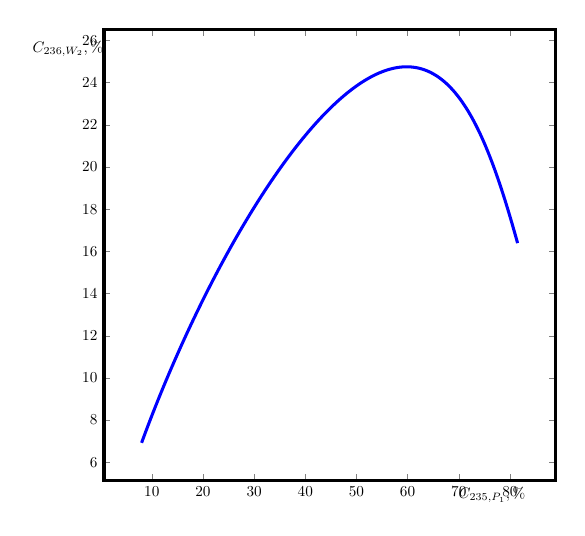
\begin{tikzpicture}[,
scale=0.55]
\begin{axis}[
  xlabel style = {{at={(axis description cs:.86,0)}}},
  ylabel = {$C_{236,W_2}, \%$},
  ylabel style = {{at={(axis description cs:-0.08,.925)},rotate=270,anchor=south}},
  xlabel = {$C_{235,P_1}, \%$},
  width=12cm, height=12cm, line width=2pt
]

\addplot+[
  mark = {none}
] coordinates {
  (8.0, 6.920332652733766)
  (8.75, 7.411276680936134)
  (9.0, 7.572297908100153)
  (9.25, 7.732064351756131)
  (9.5, 7.890607999192982)
  (9.75, 8.04795897196691)
  (10.0, 8.204145663458855)
  (10.25, 8.3591948826559)
  (10.5, 8.513131974041112)
  (10.75, 8.66598092414865)
  (11.0, 8.817764463083515)
  (11.25, 8.968504150653708)
  (11.5, 9.118220459445299)
  (11.75, 9.266932847934974)
  (12.0, 9.414659824991976)
  (12.25, 9.561419017824726)
  (12.5, 9.707227216196111)
  (12.75, 9.85210047335948)
  (13.0, 9.996054010412616)
  (13.25, 10.139102455132788)
  (13.5, 10.281259664787706)
  (13.750000000000002, 10.422539239838798)
  (14.000000000000002, 10.562953681220744)
  (14.249999999999998, 10.702515287499995)
  (14.499999999999998, 10.841235752449329)
  (14.75, 10.979126254094892)
  (15.0, 11.116197603919998)
  (15.25, 11.252460065293372)
  (15.5, 11.387923527122382)
  (15.75, 11.522597473142612)
  (16.0, 11.656491016479876)
  (16.25, 11.789612887711069)
  (16.5, 11.921971488146571)
  (16.75, 12.05357489170763)
  (17.0, 12.18443085164949)
  (17.25, 12.314546799191515)
  (17.5, 12.443929932592088)
  (17.75, 12.572587098810603)
  (18.0, 12.700524938436248)
  (18.25, 12.827749817199946)
  (18.5, 12.954267849939393)
  (18.75, 13.080084926771177)
  (19.0, 13.205206684843668)
  (19.25, 13.32963864720928)
  (19.5, 13.45338591377121)
  (19.75, 13.576453570536136)
  (20.0, 13.698846460315409)
  (20.25, 13.820569227156529)
  (20.5, 13.941626314054027)
  (20.75, 14.062022011617037)
  (21.0, 14.181760441057312)
  (21.25, 14.300845527969322)
  (21.5, 14.419281009835217)
  (21.75, 14.537070644441668)
  (22.0, 14.654217838043445)
  (22.25, 14.770725975439847)
  (22.5, 14.88659814646207)
  (22.75, 15.001837487453715)
  (23.0, 15.116446882486844)
  (23.25, 15.230429144681953)
  (23.5, 15.34378689515993)
  (23.75, 15.456522698954538)
  (24.0, 15.568638968449381)
  (24.25, 15.68013799852881)
  (24.5, 15.79102192212173)
  (24.75, 15.901292773663595)
  (25.0, 16.01095273872743)
  (25.25, 16.12000339259471)
  (25.5, 16.228446606209847)
  (25.75, 16.336283995840965)
  (26.0, 16.443517073274794)
  (26.25, 16.550147264886455)
  (26.5, 16.656175923853006)
  (26.75, 16.761604312759108)
  (27.0, 16.866433532624196)
  (27.250000000000004, 16.97066466743679)
  (27.500000000000004, 17.074298624762736)
  (27.750000000000004, 17.17733634569187)
  (28.000000000000004, 17.279778556236323)
  (28.249999999999996, 17.381625930648127)
  (28.499999999999996, 17.48287912245066)
  (28.749999999999996, 17.583538631276554)
  (28.999999999999996, 17.683604897240183)
  (29.25, 17.7830781907048)
  (29.5, 17.88195885490226)
  (29.75, 17.980247069687913)
  (30.0, 18.077942952250947)
  (30.25, 18.17504645991686)
  (30.5, 18.271557568270836)
  (30.75, 18.367476192821552)
  (31.0, 18.462802004416254)
  (31.25, 18.557534827404996)
  (31.5, 18.65167420474922)
  (31.75, 18.745219761758968)
  (32.0, 18.838170849573487)
  (32.25, 18.930526963526102)
  (32.5, 19.022287443932722)
  (32.75, 19.113451423243003)
  (33.0, 19.204018279104208)
  (33.25, 19.293986815059437)
  (33.5, 19.38335624796112)
  (33.75, 19.472125490758746)
  (34.0, 19.560293373197325)
  (34.25, 19.64785870769725)
  (34.5, 19.734820239061957)
  (34.75, 19.821176479847683)
  (35.0, 19.906926164301364)
  (35.25, 19.992067650322916)
  (35.5, 20.07659940519693)
  (35.75, 20.160519777618187)
  (36.0, 20.243827002477502)
  (36.25, 20.3265192354919)
  (36.5, 20.408594605300575)
  (36.75, 20.49005115853058)
  (37.0, 20.57088676572829)
  (37.25, 20.651099323953947)
  (37.5, 20.73068668862499)
  (37.75, 20.80964647164051)
  (38.0, 20.88797636779413)
  (38.25, 20.965673835122974)
  (38.5, 21.04273644009773)
  (38.75, 21.119161506330126)
  (39.0, 21.194946348659983)
  (39.25, 21.27008814468285)
  (39.5, 21.344583997911606)
  (39.75, 21.418430957775765)
  (40.0, 21.491626035370707)
  (40.25, 21.564166042038934)
  (40.5, 21.636047784716926)
  (40.75, 21.707267834761605)
  (41.0, 21.777823044614088)
  (41.25, 21.84770947938863)
  (41.5, 21.9169239086725)
  (41.75, 21.985462566803996)
  (42.0, 22.053321621442283)
  (42.25, 22.120497110469195)
  (42.5, 22.186985121940168)
  (42.75, 22.252781574159723)
  (43.0, 22.317882330712163)
  (43.25, 22.38228285678847)
  (43.5, 22.44597905217508)
  (43.75, 22.508966096231585)
  (44.0, 22.571239607402465)
  (44.25, 22.632794759756564)
  (44.5, 22.69362666948062)
  (44.75, 22.753730435897072)
  (45.0, 22.81310094686998)
  (45.25, 22.87173297868885)
  (45.5, 22.92962131469367)
  (45.75, 22.986760328108844)
  (46.0, 23.04314466545071)
  (46.25, 23.098768219579433)
  (46.5, 23.15362556552166)
  (46.75, 23.2077107645443)
  (47.0, 23.261017302680518)
  (47.25, 23.313539243495622)
  (47.5, 23.36527004458559)
  (47.75, 23.416203716665166)
  (48.0, 23.466332743606674)
  (48.25, 23.515650333746528)
  (48.5, 23.564150175240083)
  (48.75, 23.611824398639552)
  (49.0, 23.658666208318092)
  (49.25, 23.704667902011682)
  (49.5, 23.74982178559285)
  (49.75, 23.794120156905798)
  (50.0, 23.837555005219034)
  (50.24999999999999, 23.880118073308246)
  (50.5, 23.921801029108387)
  (50.74999999999999, 23.962595334708077)
  (51.0, 24.002492321149514)
  (51.24999999999999, 24.04148296332185)
  (51.5, 24.079558099972374)
  (51.74999999999999, 24.116708365803234)
  (52.0, 24.152924259522358)
  (52.25, 24.18819609969)
  (52.5, 24.222513590274534)
  (52.75, 24.25586666338205)
  (53.0, 24.28824490399898)
  (53.25, 24.31963717190487)
  (53.5, 24.350034083038814)
  (53.75, 24.37942251846167)
  (54.0, 24.40779199540634)
  (54.25, 24.435130518830924)
  (54.50000000000001, 24.46142616312405)
  (54.75, 24.48666682459772)
  (55.00000000000001, 24.51083988680905)
  (55.25, 24.53393273432626)
  (55.50000000000001, 24.555931822702178)
  (55.75, 24.57682390287512)
  (56.00000000000001, 24.59659550058228)
  (56.25, 24.615232324008858)
  (56.49999999999999, 24.632719928799958)
  (56.75, 24.64904383430672)
  (56.99999999999999, 24.664188970834225)
  (57.25, 24.67813996318139)
  (57.49999999999999, 24.69088089077732)
  (57.75, 24.70239573475741)
  (57.99999999999999, 24.71266798215151)
  (58.25, 24.721681177586802)
  (58.5, 24.72941720144043)
  (58.75, 24.735858951194174)
  (59.0, 24.740988362202163)
  (59.25, 24.74478677239763)
  (59.5, 24.747235549228474)
  (59.75, 24.748314697205252)
  (60.0, 24.74800495474693)
  (60.25, 24.74628591679143)
  (60.5, 24.743136952246054)
  (60.75000000000001, 24.738536215089184)
  (61.0, 24.732463111107542)
  (61.25000000000001, 24.724894137833083)
  (61.5, 24.715807168592114)
  (61.75000000000001, 24.705179260328574)
  (62.0, 24.6929862385254)
  (62.25000000000001, 24.679203852106596)
  (62.5, 24.66380704297901)
  (62.74999999999999, 24.646770776888406)
  (63.0, 24.62806886305197)
  (63.24999999999999, 24.60767456354194)
  (63.5, 24.585560919180896)
  (63.74999999999999, 24.561699944747957)
  (64.0, 24.536063619713865)
  (64.25, 24.508622779753026)
  (64.5, 24.479347956477042)
  (64.75, 24.448208835772668)
  (65.0, 24.41517462515062)
  (65.25, 24.380214338826857)
  (65.5, 24.343294993519983)
  (65.75, 24.304384668060013)
  (66.0, 24.26345002115598)
  (66.25, 24.22045665916648)
  (66.5, 24.175371000338014)
  (66.75, 24.12815676201479)
  (67.0, 24.0787790085502)
  (67.25, 24.027201009201622)
  (67.5, 23.973386541949754)
  (67.75, 23.917297196227477)
  (68.0, 23.858896286464056)
  (68.25, 23.798144551891372)
  (68.5, 23.73500293704387)
  (68.75, 23.669433280194486)
  (69.0, 23.601394778595672)
  (69.25, 23.530847843452314)
  (69.5, 23.45775246408014)
  (69.75, 23.38206790685027)
  (70.0, 23.30375321476804)
  (70.25, 23.222767680143257)
  (70.5, 23.139070327359136)
  (70.75, 23.052621388191476)
  (71.0, 22.963379232735125)
  (71.25, 22.871304118087217)
  (71.5, 22.776356089440657)
  (71.75, 22.678495363669477)
  (72.0, 22.577683671970263)
  (72.25, 22.473882765503234)
  (72.5, 22.367055270233916)
  (72.75, 22.257165807108674)
  (73.0, 22.14417884968024)
  (73.25, 22.02806128090269)
  (73.5, 21.90878091605226)
  (73.75, 21.78630936818316)
  (74.0, 21.660616993115674)
  (74.25, 21.531678228590483)
  (74.5, 21.399469999670053)
  (74.75, 21.26397106828721)
  (75.0, 21.125163963901908)
  (75.25, 20.983033296173065)
  (75.5, 20.83756751052437)
  (75.75, 20.6887585438384)
  (76.0, 20.53660194776156)
  (76.25, 20.38109713681586)
  (76.5, 20.22224694407608)
  (76.75, 20.060059795917766)
  (77.0, 19.894547054695042)
  (77.25, 19.725725600015913)
  (77.5, 19.553616587185815)
  (77.75, 19.378246535567936)
  (78.0, 19.19964504342658)
  (78.25, 19.017848871973865)
  (78.5, 18.832897388985348)
  (78.75, 18.644835835172003)
  (79.0, 18.453714772939993)
  (79.25, 18.259587491716577)
  (79.5, 18.06251348905252)
  (79.75, 17.862555879239896)
  (80.0, 17.659779856267495)
  (80.25, 17.45426102835835)
  (80.5, 17.246069291852876)
  (80.75, 17.035283638751476)
  (81.0, 16.821984908189414)
  (81.25, 16.606255659586267)
  (81.5, 16.38818101795962)
};

\end{axis}
\end{tikzpicture}


\caption{{Зависимость  концентрации $^{236}$U в потоке $W_2$ от концентрации $^{235}$U в потоке легкой фракции первого каскада ($P_1$){\label{C236W2}}}}
    \end{minipage}%
    \begin{minipage}{.5\textwidth}
      \centering
      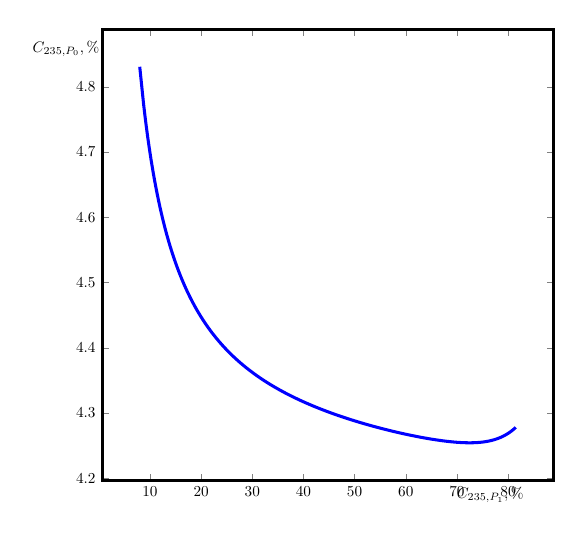
\begin{tikzpicture}[,
scale=0.55]
\begin{axis}[
  xlabel style = {{at={(axis description cs:.86,0)}}},
  ylabel = {$C_{235,P_0}, \%$},
  ylabel style = {{at={(axis description cs:-0.08,.925)},rotate=270,anchor=south}},
  xlabel = {$C_{235,P_1}, \%$},
  width=12cm, height=12cm, line width=2pt
]

\addplot+[
  mark = {none}
] coordinates {
  (8.0, 4.830477232770815)
  (8.75, 4.773408413077493)
  (9.0, 4.756696373034332)
  (9.25, 4.740966407510215)
  (9.5, 4.7261327683742)
  (9.75, 4.7121194275114595)
  (10.0, 4.698858778017614)
  (10.25, 4.686290505985744)
  (10.5, 4.674360538865699)
  (10.75, 4.663020386534869)
  (11.0, 4.652226349075555)
  (11.25, 4.641938959379373)
  (11.5, 4.632122489040375)
  (11.75, 4.622744503887625)
  (12.0, 4.613775515361663)
  (12.25, 4.6051886216294236)
  (12.5, 4.596959222220753)
  (12.75, 4.589064877852303)
  (13.0, 4.581484896510244)
  (13.25, 4.574200330550376)
  (13.5, 4.567193715352593)
  (13.750000000000002, 4.560448930986348)
  (14.000000000000002, 4.553951126810355)
  (14.249999999999998, 4.547686530072015)
  (14.499999999999998, 4.54164238043574)
  (14.75, 4.535806849899593)
  (15.0, 4.530168948750591)
  (15.25, 4.524718428165366)
  (15.5, 4.519445769772042)
  (15.75, 4.51434207582559)
  (16.0, 4.509399054143076)
  (16.25, 4.5046089171403)
  (16.5, 4.4999644004260135)
  (16.75, 4.495458696738091)
  (17.0, 4.491085415307905)
  (17.25, 4.486838529432908)
  (17.5, 4.482712433299561)
  (17.75, 4.478701781537961)
  (18.0, 4.474801588409823)
  (18.25, 4.471007142244328)
  (18.5, 4.467313991060636)
  (18.75, 4.463717937286857)
  (19.0, 4.460214991666738)
  (19.25, 4.456801423899009)
  (19.5, 4.453473662595937)
  (19.75, 4.450228357135289)
  (20.0, 4.447062293923819)
  (20.25, 4.443972462607468)
  (20.5, 4.440955973640366)
  (20.75, 4.438010101790564)
  (21.0, 4.435132250446409)
  (21.25, 4.432319945994906)
  (21.5, 4.429570837774728)
  (21.75, 4.426882690353464)
  (22.0, 4.424253360566081)
  (22.25, 4.421680838737644)
  (22.5, 4.419163135105472)
  (22.75, 4.416698435119279)
  (23.0, 4.414284950041442)
  (23.25, 4.411921000558302)
  (23.5, 4.409604953025302)
  (23.75, 4.407335270186316)
  (24.0, 4.405110473206609)
  (24.25, 4.402929139014674)
  (24.5, 4.400789893115576)
  (24.75, 4.398691421650207)
  (25.0, 4.39663256113354)
  (25.25, 4.394612012540117)
  (25.5, 4.39262867357151)
  (25.75, 4.390681431202973)
  (26.0, 4.388769219805484)
  (26.25, 4.386891015197227)
  (26.5, 4.385045844436827)
  (26.75, 4.3832327729344245)
  (27.0, 4.381450879460884)
  (27.250000000000004, 4.379699302568591)
  (27.500000000000004, 4.377977185206221)
  (27.750000000000004, 4.376283741137567)
  (28.000000000000004, 4.374618174912348)
  (28.249999999999996, 4.372979731532165)
  (28.499999999999996, 4.371367697705695)
  (28.749999999999996, 4.369781373122578)
  (28.999999999999996, 4.3682200823870945)
  (29.25, 4.3666831571098195)
  (29.5, 4.365169987453084)
  (29.75, 4.363679965574928)
  (30.0, 4.362212509241253)
  (30.25, 4.360767038428985)
  (30.5, 4.359343011747818)
  (30.75, 4.357939913471273)
  (31.0, 4.356557206712289)
  (31.25, 4.355194421760942)
  (31.5, 4.353851062032886)
  (31.75, 4.352526680011472)
  (32.0, 4.351220800643607)
  (32.25, 4.349933012009872)
  (32.5, 4.348662894824715)
  (32.75, 4.347410020255548)
  (33.0, 4.346174034463938)
  (33.25, 4.344954498858409)
  (33.5, 4.343751080626043)
  (33.75, 4.342563414349225)
  (34.0, 4.341391143707904)
  (34.25, 4.340233935764282)
  (34.5, 4.339091466943732)
  (34.75, 4.337963395442734)
  (35.0, 4.3368494430814)
  (35.25, 4.335749285574629)
  (35.5, 4.334662645076447)
  (35.75, 4.333589236155051)
  (36.0, 4.332528782864862)
  (36.25, 4.331481013718819)
  (36.5, 4.330445673461374)
  (36.75, 4.329422512997494)
  (37.0, 4.328411276302616)
  (37.25, 4.327411729780421)
  (37.5, 4.326423651531253)
  (37.75, 4.325446803422409)
  (38.0, 4.324480973983621)
  (38.25, 4.323525940878041)
  (38.5, 4.322581510713055)
  (38.75, 4.321647473726586)
  (39.0, 4.320723635797903)
  (39.25, 4.31980980176723)
  (39.5, 4.318905784988047)
  (39.75, 4.318011404149823)
  (40.0, 4.317126491553832)
  (40.25, 4.31625087130809)
  (40.5, 4.31538437882477)
  (40.75, 4.314526839359887)
  (41.0, 4.313678125731455)
  (41.25, 4.312838031940741)
  (41.5, 4.312006452140334)
  (41.75, 4.311183231450446)
  (42.0, 4.310368222991202)
  (42.25, 4.309561280318416)
  (42.5, 4.308762276773097)
  (42.75, 4.307971081258942)
  (43.0, 4.307187572826425)
  (43.25, 4.306411601037758)
  (43.5, 4.3056430770914345)
  (43.75, 4.304881849906698)
  (44.0, 4.304127830051144)
  (44.25, 4.303380895150374)
  (44.5, 4.302640932135807)
  (44.75, 4.301907842990909)
  (45.0, 4.301181518872527)
  (45.25, 4.300461857984447)
  (45.5, 4.29974877274678)
  (45.75, 4.299042150072404)
  (46.0, 4.298341918517664)
  (46.25, 4.297647948627539)
  (46.5, 4.296960192705694)
  (46.75, 4.2962785672575565)
  (47.0, 4.295602951120381)
  (47.25, 4.29493329290988)
  (47.5, 4.294269499620508)
  (47.75, 4.293611458278931)
  (48.0, 4.292959185970051)
  (48.25, 4.292312534865504)
  (48.5, 4.291671494803966)
  (48.75, 4.2910359356508545)
  (49.0, 4.290405836397011)
  (49.25, 4.289781113733665)
  (49.5, 4.289161701982779)
  (49.75, 4.288547551589692)
  (50.0, 4.287938603429412)
  (50.24999999999999, 4.287334794963874)
  (50.5, 4.286736074914972)
  (50.74999999999999, 4.286142392180261)
  (51.0, 4.285553702859666)
  (51.24999999999999, 4.28496995177237)
  (51.5, 4.284391091163391)
  (51.74999999999999, 4.283817075573771)
  (52.0, 4.283247866704502)
  (52.25, 4.282683431979082)
  (52.5, 4.282123709008566)
  (52.75, 4.281568673364692)
  (53.0, 4.281018293258683)
  (53.25, 4.280472501986412)
  (53.5, 4.279931386539307)
  (53.75, 4.2793947711457685)
  (54.0, 4.278862699898096)
  (54.25, 4.278335125637029)
  (54.50000000000001, 4.277812030560327)
  (54.75, 4.277293401632119)
  (55.00000000000001, 4.276779214412203)
  (55.25, 4.276269463527186)
  (55.50000000000001, 4.275764103892984)
  (55.75, 4.275263134090783)
  (56.00000000000001, 4.27476655997716)
  (56.25, 4.274274355130263)
  (56.49999999999999, 4.273786504954034)
  (56.75, 4.273303021844973)
  (56.99999999999999, 4.272823901541605)
  (57.25, 4.272349144706118)
  (57.49999999999999, 4.2718787396822595)
  (57.75, 4.271412698960705)
  (57.99999999999999, 4.270951028814292)
  (58.25, 4.27049376636859)
  (58.5, 4.270040867265935)
  (58.75, 4.269592382227663)
  (59.0, 4.269148333924568)
  (59.25, 4.268708730955216)
  (59.5, 4.268273617608447)
  (59.75, 4.267842980154582)
  (60.0, 4.26741688675366)
  (60.25, 4.266995362711494)
  (60.5, 4.266578453579041)
  (60.75000000000001, 4.266166162014404)
  (61.0, 4.265758605903767)
  (61.25000000000001, 4.265355751882109)
  (61.5, 4.264957693465244)
  (61.75000000000001, 4.264564508114535)
  (62.0, 4.264176234216721)
  (62.25000000000001, 4.2637929432105315)
  (62.5, 4.263414696604036)
  (62.74999999999999, 4.263041597159252)
  (63.0, 4.262673716570863)
  (63.24999999999999, 4.262311133050664)
  (63.5, 4.261953955213293)
  (63.74999999999999, 4.261602270708501)
  (64.0, 4.26125620741226)
  (64.25, 4.260915868521006)
  (64.5, 4.260581382133901)
  (64.75, 4.260252871618715)
  (65.0, 4.2599304776639695)
  (65.25, 4.2596143722108275)
  (65.5, 4.259304654227095)
  (65.75, 4.25900153700535)
  (66.0, 4.25870519342172)
  (66.25, 4.258415779155291)
  (66.5, 4.258133549268023)
  (66.75, 4.257858643455486)
  (67.0, 4.257591330532069)
  (67.25, 4.257331819240431)
  (67.5, 4.257080396747521)
  (67.75, 4.256837266330553)
  (68.0, 4.2566027797125185)
  (68.25, 4.256377181614524)
  (68.5, 4.256160776063337)
  (68.75, 4.2559539600026)
  (69.0, 4.255757017322019)
  (69.25, 4.255570344862101)
  (69.5, 4.255394352634301)
  (69.75, 4.255229444344136)
  (70.0, 4.2550760450402985)
  (70.25, 4.254934624482405)
  (70.5, 4.254805666887538)
  (70.75, 4.2546897480041626)
  (71.0, 4.254587356898545)
  (71.25, 4.2544991112491)
  (71.5, 4.254425627580807)
  (71.75, 4.254367536447987)
  (72.0, 4.254325559265821)
  (72.25, 4.254300414560013)
  (72.5, 4.2542928610692154)
  (72.75, 4.254303755147866)
  (73.0, 4.254333917011449)
  (73.25, 4.254384278860096)
  (73.5, 4.254455784869022)
  (73.75, 4.25454955161873)
  (74.0, 4.254666563215031)
  (74.25, 4.254807981518409)
  (74.5, 4.254975023216378)
  (74.75, 4.255168949604554)
  (75.0, 4.255391127000721)
  (75.25, 4.255642956481385)
  (75.5, 4.255925942215308)
  (75.75, 4.256241679303482)
  (76.0, 4.256591842345468)
  (76.25, 4.256978203223839)
  (76.5, 4.257402589923503)
  (76.75, 4.257867015061569)
  (77.0, 4.258373511765695)
  (77.25, 4.258924294401735)
  (77.5, 4.259521666599916)
  (77.75, 4.2601681142754115)
  (78.0, 4.260866138072226)
  (78.25, 4.261618513436067)
  (78.5, 4.262428104619668)
  (78.75, 4.263297936525797)
  (79.0, 4.264231291017329)
  (79.25, 4.265231459192543)
  (79.5, 4.266302098547184)
  (79.75, 4.267446940236564)
  (80.0, 4.268670008249702)
  (80.25, 4.269975852771868)
  (80.5, 4.271368698935149)
  (80.75, 4.272853540717398)
  (81.0, 4.274435396471896)
  (81.25, 4.276119771645166)
  (81.5, 4.277912480688567)
};

\end{axis}
\end{tikzpicture}


\caption{{Зависимость концентрации $^{235}$U в НОУ-разбавителе от концентрации $^{235}$U в потоке легкой фракции первого каскада ($P_1$){\label{C235P0}}}}
\end{minipage}
\end{figure}


\begin{figure}[ht]
    \centering
    \begin{minipage}{.5\textwidth}
      \centering
      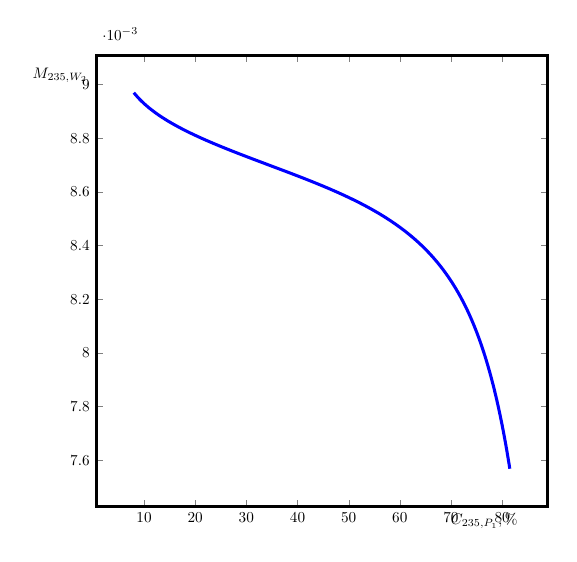
\begin{tikzpicture}[,
scale=0.55]
\begin{axis}[
  xlabel style = {{at={(axis description cs:.86,0)}}},
  ylabel = {$M_{235,W_2}$},
  ylabel style = {{at={(axis description cs:-0.08,.925)},rotate=270,anchor=south}},
  xlabel = {$C_{235,P_1}, \%$},
  width=12cm, height=12cm, line width=2pt
]

\addplot+[
  mark = {none}
] coordinates {
  (8.0, 0.008969582934887354)
  (8.75, 0.008953050957470687)
  (9.0, 0.008947961457989935)
  (9.25, 0.008943055236043482)
  (9.5, 0.008938318351511982)
  (9.75, 0.008933738550573236)
  (10.0, 0.008929304579336527)
  (10.25, 0.00892500600276735)
  (10.5, 0.008920834068883481)
  (10.75, 0.008916780111045451)
  (11.0, 0.008912836522459945)
  (11.25, 0.00890899638778039)
  (11.5, 0.008905253328491191)
  (11.75, 0.00890160156292447)
  (12.0, 0.008898035595833407)
  (12.25, 0.008894550529189556)
  (12.5, 0.008891142055842764)
  (12.75, 0.008887805346784065)
  (13.0, 0.00888453702453666)
  (13.25, 0.00888133327101651)
  (13.5, 0.008878190722767425)
  (13.750000000000002, 0.008875106482081157)
  (14.000000000000002, 0.008872077308430648)
  (14.249999999999998, 0.008869100608211533)
  (14.499999999999998, 0.008866173925463825)
  (14.75, 0.008863294824375137)
  (15.0, 0.00886046103386761)
  (15.25, 0.008857670643016527)
  (15.5, 0.0088549215481551)
  (15.75, 0.008852211964820795)
  (16.0, 0.008849540023391618)
  (16.25, 0.00884690431436794)
  (16.5, 0.008844303237468832)
  (16.75, 0.008841735275167406)
  (17.0, 0.008839199039822518)
  (17.25, 0.008836693480195931)
  (17.5, 0.00883421697699065)
  (17.75, 0.0088317687332981)
  (18.0, 0.00882934748342718)
  (18.25, 0.00882695214685525)
  (18.5, 0.008824581764264412)
  (18.75, 0.008822235354809235)
  (19.0, 0.008819912216795097)
  (19.25, 0.00881761123796545)
  (19.5, 0.008815331753722773)
  (19.75, 0.00881307281029624)
  (20.0, 0.008810833888339926)
  (20.25, 0.008808614074903603)
  (20.5, 0.008806412834731561)
  (20.75, 0.008804229443483637)
  (21.0, 0.008802063270662694)
  (21.25, 0.008799913744817398)
  (21.5, 0.00879778027046047)
  (21.75, 0.008795662265158915)
  (22.0, 0.008793559276179001)
  (22.25, 0.00879147051686481)
  (22.5, 0.008789395993835127)
  (22.75, 0.008787334812847844)
  (23.0, 0.008785286700981111)
  (23.25, 0.008783251073485748)
  (23.5, 0.008781227661490464)
  (23.75, 0.008779215933748342)
  (24.0, 0.008777215454272918)
  (24.25, 0.008775225876559527)
  (24.5, 0.008773246979830614)
  (24.75, 0.008771278510945961)
  (25.0, 0.008769319200942987)
  (25.25, 0.008767369764545823)
  (25.5, 0.008765429352778268)
  (25.75, 0.008763497724964686)
  (26.0, 0.00876157460680785)
  (26.25, 0.008759659733538669)
  (26.5, 0.008757752721138398)
  (26.75, 0.008755853183943181)
  (27.0, 0.008753960981176848)
  (27.250000000000004, 0.008752075704564152)
  (27.500000000000004, 0.008750197251064693)
  (27.750000000000004, 0.008748325098700112)
  (28.000000000000004, 0.008746459143606207)
  (28.249999999999996, 0.008744599156599683)
  (28.499999999999996, 0.00874274475756152)
  (28.749999999999996, 0.00874089570432083)
  (28.999999999999996, 0.008739051758361226)
  (29.25, 0.008737212859217611)
  (29.5, 0.008735378568265433)
  (29.75, 0.008733548658001515)
  (30.0, 0.008731722851187139)
  (30.25, 0.008729901060330605)
  (30.5, 0.008728082992807404)
  (30.75, 0.008726268277156625)
  (31.0, 0.008724456956166039)
  (31.25, 0.008722648537674339)
  (31.5, 0.00872084298824132)
  (31.75, 0.008719039917813124)
  (32.0, 0.008717239389980553)
  (32.25, 0.008715440946923838)
  (32.5, 0.008713644358357074)
  (32.75, 0.008711849635932507)
  (33.0, 0.00871005612709628)
  (33.25, 0.008708264214899087)
  (33.5, 0.00870647327897643)
  (33.75, 0.008704683167840163)
  (34.0, 0.008702893749631745)
  (34.25, 0.008701104753714752)
  (34.5, 0.008699315918146305)
  (34.75, 0.008697527280060588)
  (35.0, 0.008695738295444984)
  (35.25, 0.008693949011086596)
  (35.5, 0.008692159067325417)
  (35.75, 0.008690368279467689)
  (36.0, 0.008688576444007815)
  (36.25, 0.008686783394698666)
  (36.5, 0.008684988871695434)
  (36.75, 0.008683192626879025)
  (37.0, 0.008681394560566527)
  (37.25, 0.008679594405661325)
  (37.5, 0.008677791839637863)
  (37.75, 0.00867598678009571)
  (38.0, 0.008674178926183503)
  (38.25, 0.008672368153057894)
  (38.5, 0.008670554088754482)
  (38.75, 0.0086687365946658)
  (39.0, 0.008666915421462824)
  (39.25, 0.008665090385095373)
  (39.5, 0.008663261262198822)
  (39.75, 0.008661427825532907)
  (40.0, 0.008659589749934544)
  (40.25, 0.008657746844634986)
  (40.5, 0.008655898846421654)
  (40.75, 0.00865404564337099)
  (41.0, 0.008652186658828356)
  (41.25, 0.008650322200803322)
  (41.5, 0.008648451545630592)
  (41.75, 0.008646574533356776)
  (42.0, 0.008644690955891309)
  (42.25, 0.008642800636894704)
  (42.5, 0.008640903224070825)
  (42.75, 0.00863899844671149)
  (43.0, 0.008637085957510716)
  (43.25, 0.00863516575727924)
  (43.5, 0.008633237218089401)
  (43.75, 0.008631300408230349)
  (44.0, 0.008629354764905747)
  (44.25, 0.008627400106242656)
  (44.5, 0.008625436177556048)
  (44.75, 0.0086234625877378)
  (45.0, 0.00862147908941806)
  (45.25, 0.008619485381956294)
  (45.5, 0.008617481036809113)
  (45.75, 0.008615465921339726)
  (46.0, 0.008613439478955834)
  (46.25, 0.008611401795773408)
  (46.5, 0.008609352102023984)
  (46.75, 0.008607290031975672)
  (47.0, 0.008605215642082472)
  (47.25, 0.008603128259590765)
  (47.5, 0.008601027675848224)
  (47.75, 0.008598913983259165)
  (48.0, 0.008596785691386668)
  (48.25, 0.008594643293756862)
  (48.5, 0.008592485759095589)
  (48.75, 0.008590313355086041)
  (49.0, 0.0085881251954436)
  (49.25, 0.008585921074581795)
  (49.5, 0.008583700611067892)
  (49.75, 0.008581463263063322)
  (50.0, 0.008579208603379272)
  (50.24999999999999, 0.008576936252814263)
  (50.5, 0.008574645722361236)
  (50.74999999999999, 0.008572336531763418)
  (51.0, 0.008570008133297382)
  (51.24999999999999, 0.00856766010981354)
  (51.5, 0.008565291973522108)
  (51.74999999999999, 0.008562903220451633)
  (52.0, 0.008560493278454286)
  (52.25, 0.00855806152083667)
  (52.5, 0.0085556076484768)
  (52.75, 0.008553130961714709)
  (53.0, 0.008550630846209386)
  (53.25, 0.00854810706771584)
  (53.5, 0.00854555774925702)
  (53.75, 0.0085429838369619)
  (54.0, 0.008540383924706487)
  (54.25, 0.008537757588306388)
  (54.50000000000001, 0.008535104091081134)
  (54.75, 0.008532422651702221)
  (55.00000000000001, 0.008529712611513763)
  (55.25, 0.008526973112919355)
  (55.50000000000001, 0.008524203723571044)
  (55.75, 0.008521403545945452)
  (56.00000000000001, 0.008518571606366723)
  (56.25, 0.00851570727763321)
  (56.49999999999999, 0.008512809808569574)
  (56.75, 0.008509878155889035)
  (56.99999999999999, 0.008506911456068385)
  (57.25, 0.008503908792779345)
  (57.49999999999999, 0.00850086938251702)
  (57.75, 0.008497792179323343)
  (57.99999999999999, 0.008494676202933862)
  (58.25, 0.008491520141475806)
  (58.5, 0.008488323553930758)
  (58.75, 0.008485084979440822)
  (59.0, 0.008481803250545655)
  (59.25, 0.008478477351644427)
  (59.5, 0.008475105879196487)
  (59.75, 0.008471688048711791)
  (60.0, 0.008468222192560626)
  (60.25, 0.008464707099481916)
  (60.5, 0.00846114133577974)
  (60.75000000000001, 0.008457523922427972)
  (61.0, 0.008453852639556711)
  (61.25000000000001, 0.00845012688494179)
  (61.5, 0.008446344688200533)
  (61.75000000000001, 0.008442504246032677)
  (62.0, 0.008438604167544233)
  (62.25000000000001, 0.008434642701742214)
  (62.5, 0.00843061819667875)
  (62.74999999999999, 0.008426528551434788)
  (63.0, 0.008422371991251038)
  (63.24999999999999, 0.008418146665359498)
  (63.5, 0.008413850388432755)
  (63.74999999999999, 0.008409481193270963)
  (64.0, 0.00840503667489769)
  (64.25, 0.008400514684896585)
  (64.5, 0.00839591280165317)
  (64.75, 0.008391228646229737)
  (65.0, 0.008386459646753221)
  (65.25, 0.008381602891968784)
  (65.5, 0.008376656246177845)
  (65.75, 0.008371616339520984)
  (66.0, 0.008366480231628762)
  (66.25, 0.008361245162791847)
  (66.5, 0.008355907301054039)
  (66.75, 0.00835046404896195)
  (67.0, 0.008344911421099945)
  (67.25, 0.008339246074549682)
  (67.5, 0.008333463823960592)
  (67.75, 0.008327561384019997)
  (68.0, 0.008321533879538923)
  (68.25, 0.00831537758511544)
  (68.5, 0.00830908814223659)
  (68.75, 0.008302660204893444)
  (69.0, 0.008296089646192446)
  (69.25, 0.00828937113819764)
  (69.5, 0.008282499224605326)
  (69.75, 0.008275468531667402)
  (70.0, 0.00826827347415231)
  (70.25, 0.008260908009095722)
  (70.5, 0.00825336596088543)
  (70.75, 0.008245640203393603)
  (71.0, 0.008237724568319199)
  (71.25, 0.00822961154384384)
  (71.5, 0.008221293669866929)
  (71.75, 0.00821276338124383)
  (72.0, 0.008204012187817605)
  (72.25, 0.00819503168306494)
  (72.5, 0.008185813088394164)
  (72.75, 0.008176346645735303)
  (73.0, 0.00816662305461966)
  (73.25, 0.008156631890100853)
  (73.5, 0.008146362682047308)
  (73.75, 0.008135803206441633)
  (74.0, 0.008124942750070615)
  (74.25, 0.008113768797907307)
  (74.5, 0.008102268366638297)
  (74.75, 0.00809042809718903)
  (75.0, 0.008078233643784233)
  (75.25, 0.008065670407119764)
  (75.5, 0.008052722827568548)
  (75.75, 0.008039374511333873)
  (76.0, 0.00802560836493737)
  (76.25, 0.008011406404869104)
  (76.5, 0.007996750206473837)
  (76.75, 0.00798161953598353)
  (77.0, 0.007965994104478175)
  (77.25, 0.007949851853015227)
  (77.5, 0.007933169944668625)
  (77.75, 0.007915923760480153)
  (78.0, 0.007898088701745708)
  (78.25, 0.007879637419106009)
  (78.5, 0.00786054173728438)
  (78.75, 0.007840771975822277)
  (79.0, 0.00782029584895143)
  (79.25, 0.0077990811576082175)
  (79.5, 0.007777091914924569)
  (79.75, 0.00775429154132833)
  (80.0, 0.007730640361314449)
  (80.25, 0.007706093308217856)
  (80.5, 0.00768060886945932)
  (80.75, 0.007654137404335572)
  (81.0, 0.007626629210857389)
  (81.25, 0.007598029377462495)
  (81.5, 0.00756827981297914)
};

\end{axis}
\end{tikzpicture}


\caption{{Зависимость массы $^{235}$U в потоке тяжелой фракции второго каскада $W_2$ от концентрации $^{235}$U в потоке легкой фракции первого каскада{\label{M235W2}}}}
    \end{minipage}%
    \begin{minipage}{.5\textwidth}
      \centering
      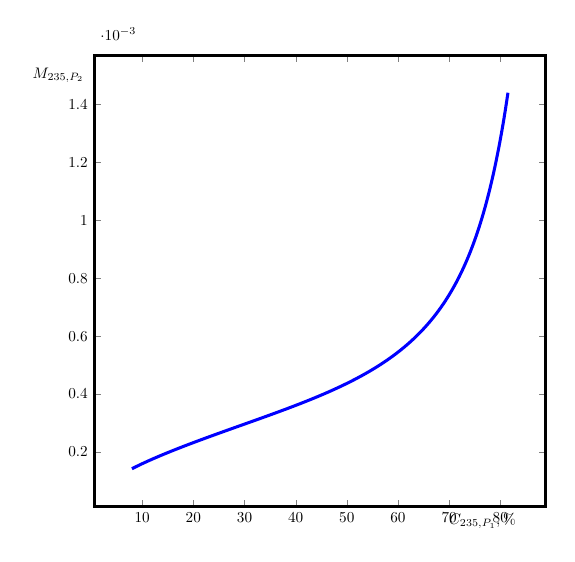
\begin{tikzpicture}[,
scale=0.55]
\begin{axis}[
  xlabel style = {{at={(axis description cs:.86,0)}}},
  ylabel = {$M_{235,P_2}$},
  ylabel style = {{at={(axis description cs:-0.08,.925)},rotate=270,anchor=south}},
  xlabel = {$C_{235,P_1}, \%$},
  width=12cm, height=12cm, line width=2pt
]

\addplot+[
  mark = {none}
] coordinates {
  (8.0, 0.00014206261852688643)
  (8.75, 0.0001487192550358152)
  (9.0, 0.00015088683708154766)
  (9.25, 0.00015303080917051723)
  (9.5, 0.0001551523719881621)
  (9.75, 0.00015725236007136956)
  (10.0, 0.0001593317614887236)
  (10.25, 0.00016139175686364607)
  (10.5, 0.00016343273361451926)
  (10.75, 0.0001654557792220484)
  (11.0, 0.0001674616166564755)
  (11.25, 0.00016945089482455766)
  (11.5, 0.00017142427548982213)
  (11.75, 0.00017338231427642395)
  (12.0, 0.00017532571955085064)
  (12.25, 0.00017725499644316329)
  (12.5, 0.00017917041347116197)
  (12.75, 0.00018107311175734472)
  (13.0, 0.00018296297550549672)
  (13.25, 0.00018484068339518633)
  (13.5, 0.00018670656510795378)
  (13.750000000000002, 0.00018856109931456714)
  (14.000000000000002, 0.00019040470599054806)
  (14.249999999999998, 0.00019223773103972837)
  (14.499999999999998, 0.00019406044955978683)
  (14.75, 0.00019587322712990587)
  (15.0, 0.00019767651210762089)
  (15.25, 0.00019947040749950323)
  (15.5, 0.0002012553606385691)
  (15.75, 0.000203031605489627)
  (16.0, 0.0002047995586925459)
  (16.25, 0.00020655926673278035)
  (16.5, 0.00020831104998772658)
  (16.75, 0.00021005522295182956)
  (17.0, 0.00021179204141915403)
  (17.25, 0.00021352149077778944)
  (17.5, 0.00021524418573034358)
  (17.75, 0.00021695997550854248)
  (18.0, 0.00021866923106948102)
  (18.25, 0.00022037218749844817)
  (18.5, 0.0002220690046236574)
  (18.75, 0.00022375990666895904)
  (19.0, 0.00022544487874026487)
  (19.25, 0.00022712440176520985)
  (19.5, 0.000228798400960687)
  (19.75, 0.0002304672501441958)
  (20.0, 0.00023213092387050163)
  (20.25, 0.00023378975969221073)
  (20.5, 0.00023544377445984787)
  (20.75, 0.00023709318868042308)
  (21.0, 0.00023873816478958473)
  (21.25, 0.00024037880841981435)
  (21.5, 0.0002420152389167409)
  (21.75, 0.0002436477293426275)
  (22.0, 0.00024527628827047715)
  (22.25, 0.00024690132702418757)
  (22.5, 0.000248522480408844)
  (22.75, 0.0002501402999215804)
  (23.0, 0.00025175473070630355)
  (23.25, 0.00025336604389309693)
  (23.5, 0.00025497420813668046)
  (23.75, 0.0002565794671615227)
  (24.0, 0.00025818198146186926)
  (24.25, 0.00025978183345767603)
  (24.5, 0.00026137899066494216)
  (24.75, 0.00026297346323659904)
  (25.0, 0.00026456628690646705)
  (25.25, 0.0002661565229951418)
  (25.5, 0.0002677448053406744)
  (25.75, 0.000269331167867999)
  (26.0, 0.0002709156861062661)
  (26.25, 0.00027249843365755483)
  (26.5, 0.0002740796106147544)
  (26.75, 0.00027565942561739483)
  (27.0, 0.00027723784899813124)
  (27.250000000000004, 0.0002788151248665254)
  (27.500000000000004, 0.0002803911980887289)
  (27.750000000000004, 0.0002819664381894382)
  (28.000000000000004, 0.00028354080204344467)
  (28.249999999999996, 0.00028511437706629176)
  (28.499999999999996, 0.0002866874066010505)
  (28.749999999999996, 0.00028826000081666806)
  (28.999999999999996, 0.00028983227079514023)
  (29.25, 0.00029140415393881665)
  (29.5, 0.00029297596999531867)
  (29.75, 0.0002945478316002078)
  (30.0, 0.00029611990496630937)
  (30.25, 0.0002976921702418694)
  (30.5, 0.00029926481623896936)
  (30.75, 0.00030083811399311594)
  (31.0, 0.0003024119235411315)
  (31.25, 0.0003039866429885015)
  (31.5, 0.00030556221471501877)
  (31.75, 0.0003071389405912217)
  (32.0, 0.00030871667160734965)
  (32.25, 0.0003102957828210971)
  (32.5, 0.00031187642431066976)
  (32.75, 0.00031345850667270484)
  (33.0, 0.0003150426070731949)
  (33.25, 0.0003166282693477201)
  (33.5, 0.00031821604293607675)
  (33.75, 0.00031980601050942775)
  (34.0, 0.0003213982371393116)
  (34.25, 0.00032299292863086315)
  (34.5, 0.00032459028398027255)
  (34.75, 0.0003261902049233192)
  (35.0, 0.0003277931760941529)
  (35.25, 0.0003293990930164905)
  (35.5, 0.0003310082592907783)
  (35.75, 0.00033262080512371883)
  (36.0, 0.0003342368810515949)
  (36.25, 0.00033585660181746966)
  (36.5, 0.0003374801771770407)
  (36.75, 0.00033910780652696257)
  (37.0, 0.0003407395421480962)
  (37.25, 0.0003423756050109775)
  (37.5, 0.0003440162727483667)
  (37.75, 0.0003456615840602884)
  (38.0, 0.00034731179725073575)
  (38.25, 0.00034896699573092933)
  (38.5, 0.0003506275111121188)
  (38.75, 0.0003522934426926643)
  (39.0, 0.00035396500150299795)
  (39.25, 0.0003556423342729505)
  (39.5, 0.0003573256279940082)
  (39.75, 0.00035901507445064196)
  (40.0, 0.0003607109642387537)
  (40.25, 0.0003624134510816995)
  (40.5, 0.00036412276709177246)
  (40.75, 0.0003658389932795444)
  (41.0, 0.0003675626749870876)
  (41.25, 0.00036929347365014225)
  (41.5, 0.00037103208311411453)
  (41.75, 0.00037277863422507766)
  (42.0, 0.00037453330665735036)
  (42.25, 0.0003762962490045512)
  (42.5, 0.00037806778646733223)
  (42.75, 0.00037984816328946784)
  (43.0, 0.0003816377009249703)
  (43.25, 0.00038343637330555364)
  (43.5, 0.0003852447836783621)
  (43.75, 0.0003870628396339368)
  (44.0, 0.0003888910803922337)
  (44.25, 0.00039072966477804054)
  (44.5, 0.0003925788249412114)
  (44.75, 0.0003944389299529779)
  (45.0, 0.000396310205630296)
  (45.25, 0.00039819293153099146)
  (45.5, 0.00040008751557256785)
  (45.75, 0.00040199407020977)
  (46.0, 0.00040391313228410814)
  (46.25, 0.0004058445963478875)
  (46.5, 0.000407789213245078)
  (46.75, 0.00040974733017878527)
  (47.0, 0.00041171887255078395)
  (47.25, 0.00041370449534414876)
  (47.5, 0.00041570438980380016)
  (47.75, 0.0004177190178365665)
  (48.0, 0.00041974875542380533)
  (48.25, 0.00042179362217733245)
  (48.5, 0.00042385463351269574)
  (48.75, 0.0004259315062140724)
  (49.0, 0.00042802511135106775)
  (49.25, 0.0004301356396047288)
  (49.5, 0.0004322634578040857)
  (49.75, 0.00043440909347813053)
  (50.0, 0.0004365729597928729)
  (50.24999999999999, 0.00043875542220659535)
  (50.5, 0.00044095695625585315)
  (50.74999999999999, 0.0004431780289928668)
  (51.0, 0.00044541917519591665)
  (51.24999999999999, 0.00044768079932255096)
  (51.5, 0.0004499633767174201)
  (51.74999999999999, 0.0004522673991477988)
  (52.0, 0.00045459342679249256)
  (52.25, 0.00045694207460538074)
  (52.5, 0.00045931363019295965)
  (52.75, 0.0004617087819184397)
  (53.0, 0.0004641281330396219)
  (53.25, 0.00046657190692678724)
  (53.5, 0.0004690419698859583)
  (53.75, 0.00047153736531601004)
  (54.0, 0.00047405948906307284)
  (54.25, 0.00047660875522349496)
  (54.50000000000001, 0.0004791858905751159)
  (54.75, 0.00048179166672502986)
  (55.00000000000001, 0.00048442673278477555)
  (55.25, 0.00048709193697948)
  (55.50000000000001, 0.0004897877024549516)
  (55.75, 0.0004925149176977991)
  (56.00000000000001, 0.0004952745475087547)
  (56.25, 0.000498067210372404)
  (56.49999999999999, 0.0005008936489015665)
  (56.75, 0.0005037548979716578)
  (56.99999999999999, 0.0005066518128423399)
  (57.25, 0.0005095853017229255)
  (57.49999999999999, 0.0005125561401407897)
  (57.75, 0.0005155653662148463)
  (57.99999999999999, 0.0005186139525057761)
  (58.25, 0.0005217032033150501)
  (58.5, 0.0005248335522194126)
  (58.75, 0.0005280064527619661)
  (59.0, 0.0005312230652124307)
  (59.25, 0.0005344843981025534)
  (59.5, 0.000537791848022905)
  (59.75, 0.0005411461926299319)
  (60.0, 0.0005445490928338145)
  (60.25, 0.0005480017532877826)
  (60.5, 0.0005515056011892717)
  (60.75000000000001, 0.0005550616091730453)
  (61.0, 0.0005586719908225494)
  (61.25000000000001, 0.0005623373421782563)
  (61.5, 0.0005660596275398105)
  (61.75000000000001, 0.0005698406442230616)
  (62.0, 0.0005736817772341985)
  (62.25000000000001, 0.0005775847717730899)
  (62.5, 0.0005815512740872374)
  (62.74999999999999, 0.000585583379486238)
  (63.0, 0.000589682857209016)
  (63.24999999999999, 0.0005938515525905125)
  (63.5, 0.0005980916456106702)
  (63.74999999999999, 0.00060240509820575)
  (64.0, 0.0006067943101708379)
  (64.25, 0.0006112614248215335)
  (64.5, 0.0006158088587506189)
  (64.75, 0.0006204389859515801)
  (65.0, 0.0006251543734292362)
  (65.25, 0.0006299579276446713)
  (65.5, 0.000634851779575759)
  (65.75, 0.0006398392944328368)
  (66.0, 0.0006449234080065024)
  (66.25, 0.0006501068754961208)
  (66.5, 0.0006553935244154773)
  (66.75, 0.0006607859478417916)
  (67.0, 0.0006662881268794789)
  (67.25, 0.0006719034001993863)
  (67.5, 0.0006776359489670697)
  (67.75, 0.0006834890543714472)
  (68.0, 0.0006894675875378399)
  (68.25, 0.000695575269863432)
  (68.5, 0.0007018164559142097)
  (68.75, 0.000708196487808803)
  (69.0, 0.0007147194886059934)
  (69.25, 0.0007213907824614268)
  (69.5, 0.0007282158219518746)
  (69.75, 0.0007351999771508405)
  (70.0, 0.0007423488296665546)
  (70.25, 0.0007496684188902872)
  (70.5, 0.0007571649169104045)
  (70.75, 0.0007648454463791348)
  (71.0, 0.0007727161721691653)
  (71.25, 0.0007807846027167577)
  (71.5, 0.0007890581947856685)
  (71.75, 0.0007975445102280024)
  (72.0, 0.0008062520359515104)
  (72.25, 0.000815189175272715)
  (72.5, 0.0008243647036179145)
  (72.75, 0.0008337883759322068)
  (73.0, 0.0008434694895989494)
  (73.25, 0.0008534184665177729)
  (73.5, 0.000863645773811138)
  (73.75, 0.0008741636325240199)
  (74.0, 0.0008849827529329532)
  (74.25, 0.0008961156471629762)
  (74.5, 0.0009075752956594171)
  (74.75, 0.0009193750546615769)
  (75.0, 0.0009315292671413294)
  (75.25, 0.0009440525296302777)
  (75.5, 0.0009569603990128037)
  (75.75, 0.0009702692663717642)
  (76.0, 0.000983996222499424)
  (76.25, 0.0009981592482463631)
  (76.5, 0.001012776765634078)
  (76.75, 0.0010278690058213892)
  (77.0, 0.0010434562551424789)
  (77.25, 0.0010595605699762838)
  (77.5, 0.0010762047847062738)
  (77.75, 0.0010934135157678515)
  (78.0, 0.0011112113593608204)
  (78.25, 0.0011296260128246794)
  (78.5, 0.0011486849805324923)
  (78.75, 0.0011684182657858363)
  (79.0, 0.0011888578683866158)
  (79.25, 0.001210036389519737)
  (79.5, 0.0012319896182465644)
  (79.75, 0.0012547550672794418)
  (80.0, 0.0012783709017684958)
  (80.25, 0.001302882822164161)
  (80.5, 0.0013283323618665562)
  (80.75, 0.0013547682953359422)
  (81.0, 0.0013822419389410525)
  (81.25, 0.0014108074289008383)
  (81.5, 0.0014405228539761475)
};

\end{axis}
\end{tikzpicture}


\caption{{Зависимость массы $^{235}$U в потоке легкой фракции второго каскада $P_2$ от концентрации $^{235}$U в потоке легкой фракции первого каскада{\label{M235P2}}}}
\end{minipage}
\end{figure}


\begin{figure}[ht]
  \centering
  \begin{minipage}{.5\textwidth}
    \centering
    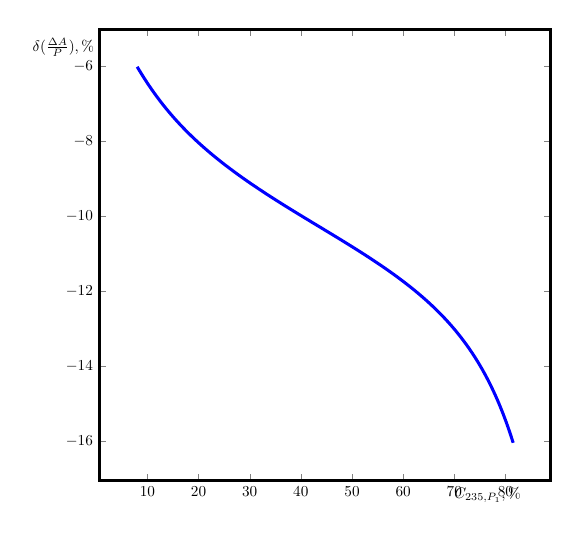
\begin{tikzpicture}[,
scale=0.55]
\begin{axis}[
  xlabel style = {{at={(axis description cs:.86,0)}}},
  ylabel = {$\delta(\frac{\Delta A}{P}), \%$},
  ylabel style = {{at={(axis description cs:-0.08,.925)},rotate=270,anchor=south}},
  xlabel = {$C_{235,P_1}, \%$},
  width=12cm, height=12cm, line width=2pt
]

\addplot+[
  mark = {none}
] coordinates {
  (8.0, -6.009073941803377)
  (8.75, -6.177258517450099)
  (9.0, -6.232024106272706)
  (9.25, -6.28608738792488)
  (9.5, -6.339430582599556)
  (9.75, -6.39204179225068)
  (10.0, -6.443915604039634)
  (10.25, -6.495052198003927)
  (10.5, -6.545452422175985)
  (10.75, -6.595123040274078)
  (11.0, -6.644071853444348)
  (11.25, -6.692308344797842)
  (11.5, -6.739843625866472)
  (11.75, -6.786689643253145)
  (12.0, -6.8328598003202154)
  (12.25, -6.878367523501224)
  (12.5, -6.92322586101102)
  (12.75, -6.967451766977895)
  (13.0, -7.011056738069472)
  (13.25, -7.0540564170650635)
  (13.5, -7.096463624350019)
  (13.750000000000002, -7.138296537755508)
  (14.000000000000002, -7.179565793108972)
  (14.249999999999998, -7.220286422544805)
  (14.499999999999998, -7.260471865597622)
  (14.75, -7.300135251149248)
  (15.0, -7.339291043405373)
  (15.25, -7.377951020720038)
  (15.5, -7.416128275827816)
  (15.75, -7.453834943177387)
  (16.0, -7.491083478496631)
  (16.25, -7.527884845037343)
  (16.5, -7.564250639563587)
  (16.75, -7.600192168909545)
  (17.0, -7.635720255259592)
  (17.25, -7.670844582068202)
  (17.5, -7.705576634432516)
  (17.75, -7.739925085679744)
  (18.0, -7.773900127470927)
  (18.25, -7.807511199387631)
  (18.5, -7.840767259161227)
  (18.75, -7.873677249754789)
  (19.0, -7.906249122085142)
  (19.25, -7.93849275200838)
  (19.5, -7.9704142502778605)
  (19.75, -8.00202252010609)
  (20.0, -8.033325042612466)
  (20.25, -8.06432951266108)
  (20.5, -8.095042768098141)
  (20.75, -8.125471988858079)
  (21.0, -8.1556241195333)
  (21.25, -8.185505498304797)
  (21.5, -8.215121958083518)
  (21.75, -8.244481437869128)
  (22.0, -8.273589015944943)
  (22.25, -8.302451476160735)
  (22.5, -8.331073042340941)
  (22.75, -8.359460645844434)
  (23.0, -8.387619211999075)
  (23.25, -8.41555450446831)
  (23.5, -8.443271230659818)
  (23.75, -8.470774840424369)
  (24.0, -8.498070354799255)
  (24.25, -8.52516250264354)
  (24.5, -8.552055496182351)
  (24.75, -8.578753593967257)
  (25.0, -8.605264017402709)
  (25.25, -8.631587956094085)
  (25.5, -8.657731219212488)
  (25.75, -8.68369772897508)
  (26.0, -8.70949140327394)
  (26.25, -8.735116111934627)
  (26.5, -8.760575978543592)
  (26.75, -8.785875068641658)
  (27.0, -8.81101667501409)
  (27.250000000000004, -8.836004800962312)
  (27.500000000000004, -8.860842515940446)
  (27.750000000000004, -8.88553403144478)
  (28.000000000000004, -8.910082292723805)
  (28.249999999999996, -8.934490548839745)
  (28.499999999999996, -8.9587624663783)
  (28.749999999999996, -8.982901198389388)
  (28.999999999999996, -9.0069098990062)
  (29.25, -9.030791107708652)
  (29.5, -9.054548452281667)
  (29.75, -9.078184884907479)
  (30.0, -9.101703452289394)
  (30.25, -9.125106598394183)
  (30.5, -9.148397355715089)
  (30.75, -9.171578904659098)
  (31.0, -9.1946532050119)
  (31.25, -9.217623731068484)
  (31.5, -9.240492579499158)
  (31.75, -9.263262843183508)
  (32.0, -9.285936288460798)
  (32.25, -9.30851611310295)
  (32.5, -9.331004870046124)
  (32.75, -9.35340435821551)
  (33.0, -9.37571824400418)
  (33.25, -9.39794721820897)
  (33.5, -9.420094799773233)
  (33.75, -9.442163142070111)
  (34.0, -9.464154323454208)
  (34.25, -9.486070766200063)
  (34.5, -9.507914860271098)
  (34.75, -9.529688133773561)
  (35.0, -9.551393704174725)
  (35.25, -9.573033032645338)
  (35.5, -9.594608641646706)
  (35.75, -9.61612262809096)
  (36.0, -9.6375770434154)
  (36.25, -9.658973848128884)
  (36.5, -9.68031523886753)
  (36.75, -9.701603362762116)
  (37.0, -9.722839923366056)
  (37.25, -9.744027082449563)
  (37.5, -9.765167140637352)
  (37.75, -9.786261694648635)
  (38.0, -9.807312973352868)
  (38.25, -9.828322640129397)
  (38.5, -9.849293073744734)
  (38.75, -9.87022598092836)
  (39.0, -9.891123366323887)
  (39.25, -9.911987030470238)
  (39.5, -9.932818852176169)
  (39.75, -9.953620751312757)
  (40.0, -9.974394879122027)
  (40.25, -9.995142939889767)
  (40.5, -10.015866941609273)
  (40.75, -10.036568416102645)
  (41.0, -10.057250186087241)
  (41.25, -10.07791259351861)
  (41.5, -10.098558839880315)
  (41.75, -10.119190549452272)
  (42.0, -10.139809468871258)
  (42.25, -10.160417248590473)
  (42.5, -10.18101603067991)
  (42.75, -10.201607723573987)
  (43.0, -10.222194424295957)
  (43.25, -10.24277726912131)
  (43.5, -10.263359134960856)
  (43.75, -10.28394095912421)
  (44.0, -10.304525422127005)
  (44.25, -10.325114151871967)
  (44.5, -10.34570897100183)
  (44.75, -10.366312052003405)
  (45.0, -10.386925212412471)
  (45.25, -10.407550376014656)
  (45.5, -10.428189830295173)
  (45.75, -10.448845045090884)
  (46.0, -10.46951865694529)
  (46.25, -10.490211535278117)
  (46.5, -10.510926890999942)
  (46.75, -10.531666836694226)
  (47.0, -10.552432319116512)
  (47.25, -10.573226284864752)
  (47.5, -10.594050415503013)
  (47.75, -10.614914525192077)
  (48.0, -10.635806587407128)
  (48.25, -10.656734666662175)
  (48.5, -10.67770270917247)
  (48.75, -10.698711091537442)
  (49.0, -10.719763367826385)
  (49.25, -10.740861228665993)
  (49.5, -10.762006850477848)
  (49.75, -10.783202850047156)
  (50.0, -10.804451538501024)
  (50.24999999999999, -10.825755101351401)
  (50.5, -10.847116028127202)
  (50.74999999999999, -10.868536793911646)
  (51.0, -10.890020060396488)
  (51.24999999999999, -10.911568144661631)
  (51.5, -10.933183562923977)
  (51.74999999999999, -10.954868881946064)
  (52.0, -10.976626869816716)
  (52.25, -10.998460438434057)
  (52.5, -11.020371634428837)
  (52.75, -11.042363594501845)
  (53.0, -11.064439236141478)
  (53.25, -11.086600458777912)
  (53.5, -11.108853606564297)
  (53.75, -11.131197421627052)
  (54.0, -11.15363701928954)
  (54.25, -11.176174866279629)
  (54.50000000000001, -11.198814263194448)
  (54.75, -11.221558690749708)
  (55.00000000000001, -11.244411274321424)
  (55.25, -11.267375733270123)
  (55.50000000000001, -11.290454617063856)
  (55.75, -11.313651761387078)
  (56.00000000000001, -11.336971228823705)
  (56.25, -11.360416157761602)
  (56.49999999999999, -11.383990069770634)
  (56.75, -11.407697245241279)
  (56.99999999999999, -11.431541518659525)
  (57.25, -11.455526892132054)
  (57.49999999999999, -11.479657054530062)
  (57.75, -11.503936384867501)
  (57.99999999999999, -11.528369115579594)
  (58.25, -11.552960404073602)
  (58.5, -11.577713092051694)
  (58.75, -11.602632804745925)
  (59.0, -11.627724342631183)
  (59.25, -11.65299218550429)
  (59.5, -11.67844185077971)
  (59.75, -11.704077242307774)
  (60.0, -11.729904634955046)
  (60.25, -11.755929132889378)
  (60.5, -11.78215645386723)
  (60.75000000000001, -11.808591132640037)
  (61.0, -11.835241036959717)
  (61.25000000000001, -11.862109781995375)
  (61.5, -11.88920462903246)
  (61.75000000000001, -11.916532439990515)
  (62.0, -11.944099010933353)
  (62.25000000000001, -11.971911139271214)
  (62.5, -11.99997538398778)
  (62.74999999999999, -12.028299532142697)
  (63.0, -12.056890541739685)
  (63.24999999999999, -12.085755621709138)
  (63.5, -12.11490288423379)
  (63.74999999999999, -12.144339908638127)
  (64.0, -12.174075479053746)
  (64.25, -12.204117727252342)
  (64.5, -12.234475556888963)
  (64.75, -12.265157782904538)
  (65.0, -12.296173762211717)
  (65.25, -12.327533813658764)
  (65.5, -12.359246243604744)
  (65.75, -12.391322614690631)
  (66.0, -12.423773416073995)
  (66.25, -12.456608715489734)
  (66.5, -12.489841404315163)
  (66.75, -12.523481182001078)
  (67.0, -12.557541417479909)
  (67.25, -12.592033830402782)
  (67.5, -12.626972371273663)
  (67.75, -12.662368666553428)
  (68.0, -12.698238534655177)
  (68.25, -12.734594803198226)
  (68.5, -12.771451956415882)
  (68.75, -12.808827105358658)
  (69.0, -12.846734175837241)
  (69.25, -12.885190235022709)
  (69.5, -12.924212690718475)
  (69.75, -12.963818732475813)
  (70.0, -13.004026088981801)
  (70.25, -13.044853677810009)
  (70.5, -13.086320721619352)
  (70.75, -13.128448925014096)
  (71.0, -13.171257437061046)
  (71.25, -13.21476885314698)
  (71.5, -13.259005579156627)
  (71.75, -13.303990248120176)
  (72.0, -13.34974781859688)
  (72.25, -13.396302933147327)
  (72.5, -13.443681099640333)
  (72.75, -13.491910273499313)
  (73.0, -13.541017101562034)
  (73.25, -13.59103098988147)
  (73.5, -13.641981314343937)
  (73.75, -13.693901858760515)
  (74.0, -13.746822276450432)
  (74.25, -13.800776676113689)
  (74.5, -13.855800273930313)
  (74.75, -13.91192886665059)
  (75.0, -13.969200727659592)
  (75.25, -14.027654404589606)
  (75.5, -14.087330736625855)
  (75.75, -14.148272395840051)
  (76.0, -14.210523597962258)
  (76.25, -14.274130517889327)
  (76.5, -14.339140162528413)
  (76.75, -14.405603909518131)
  (77.0, -14.473572927315647)
  (77.25, -14.543102595629637)
  (77.5, -14.614250019519037)
  (77.75, -14.68707648984218)
  (78.0, -14.761642976997521)
  (78.25, -14.838022805889029)
  (78.5, -14.916274771539925)
  (78.75, -14.99647715818782)
  (79.0, -15.078704933401745)
  (79.25, -15.163043606043262)
  (79.5, -15.249578534748398)
  (79.75, -15.338414596285807)
  (80.0, -15.42962509320257)
  (80.25, -15.523331540794588)
  (80.5, -15.619636306653478)
  (80.75, -15.718648234698904)
  (81.0, -15.820516302401016)
  (81.25, -15.925364251096141)
  (81.5, -16.033336546705275)
};

\end{axis}
\end{tikzpicture}


\caption{{Зависимость экономии работы разделения от концентрации $^{235}$U в потоке легкой фракции первого каскада ($P_1$){\label{SW_l}}}}
  \end{minipage}%
  \begin{minipage}{.5\textwidth}
    \centering
    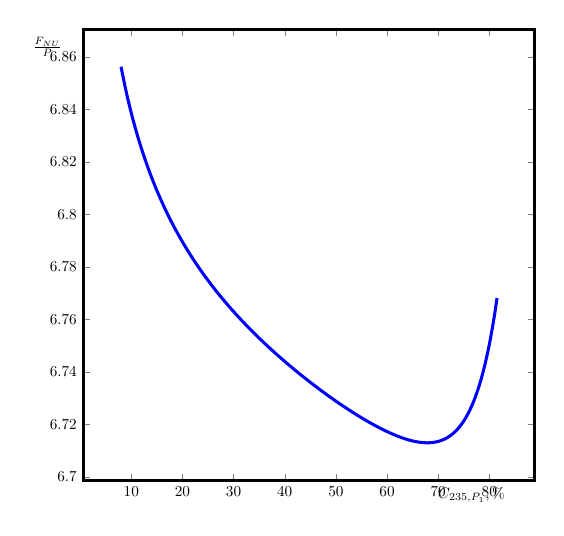
\begin{tikzpicture}[,
scale=0.55]
\begin{axis}[
  xlabel style = {{at={(axis description cs:.86,0)}}},
  ylabel = {$\frac{F_{NU}}{P}$},
  ylabel style = {{at={(axis description cs:-0.08,.925)},rotate=270,anchor=south}},
  xlabel = {$C_{235,P_1}, \%$},
  width=12cm, height=12cm, line width=2pt
]

\addplot+[
  mark = {none}
] coordinates {
  (8.0, 6.8562614710312335)
  (8.75, 6.849083351767669)
  (9.0, 6.846862757095191)
  (9.25, 6.8447189370703905)
  (9.5, 6.842647095379589)
  (9.75, 6.84064281236473)
  (10.0, 6.838702078359409)
  (10.25, 6.836821258282764)
  (10.5, 6.834996899389661)
  (10.75, 6.8332259354267215)
  (11.0, 6.8315054906948465)
  (11.25, 6.829832901446023)
  (11.5, 6.828205708170214)
  (11.75, 6.82662161780716)
  (12.0, 6.825078527582706)
  (12.25, 6.823574454211363)
  (12.5, 6.822107514968316)
  (12.75, 6.820676086950488)
  (13.0, 6.819278476202349)
  (13.25, 6.817913208316127)
  (13.5, 6.816578867632903)
  (13.750000000000002, 6.815274100681365)
  (14.000000000000002, 6.813997703162073)
  (14.249999999999998, 6.812748485075032)
  (14.499999999999998, 6.811525327806559)
  (14.75, 6.810327197249813)
  (15.0, 6.809153118321921)
  (15.25, 6.808002131933252)
  (15.5, 6.8068733806276285)
  (15.75, 6.805766021921724)
  (16.0, 6.8046792873077395)
  (16.25, 6.803612392124296)
  (16.5, 6.802564634301183)
  (16.75, 6.8015353477149025)
  (17.0, 6.8005238914031345)
  (17.25, 6.799529614096266)
  (17.5, 6.798551994180876)
  (17.75, 6.797590417479472)
  (18.0, 6.796644379178978)
  (18.25, 6.795713377932425)
  (18.5, 6.7947969241997335)
  (18.75, 6.793894560967668)
  (19.0, 6.79300581451699)
  (19.25, 6.792130302875228)
  (19.5, 6.791267593745464)
  (19.75, 6.79041732687871)
  (20.0, 6.789579095114163)
  (20.25, 6.788752572232118)
  (20.5, 6.787937392366052)
  (20.75, 6.7871332375542)
  (21.0, 6.7863397925142435)
  (21.25, 6.7855567484454955)
  (21.5, 6.784783815085504)
  (21.75, 6.784020718499905)
  (22.0, 6.783267174331568)
  (22.25, 6.782522965448584)
  (22.5, 6.781787761939818)
  (22.75, 6.7810613882612385)
  (23.0, 6.780343582126754)
  (23.25, 6.779634141191229)
  (23.5, 6.778932823525798)
  (23.75, 6.7782394386141425)
  (24.0, 6.777553789989539)
  (24.25, 6.77687567631403)
  (24.5, 6.776204884609303)
  (24.75, 6.775541215269211)
  (25.0, 6.774884636820289)
  (25.25, 6.774234811970397)
  (25.5, 6.773591657432545)
  (25.75, 6.772955000697834)
  (26.0, 6.772324680845549)
  (26.25, 6.771700541921445)
  (26.5, 6.771082452548623)
  (26.75, 6.770470287316287)
  (27.0, 6.769863887676315)
  (27.250000000000004, 6.769263142429263)
  (27.500000000000004, 6.7686678973317225)
  (27.750000000000004, 6.768078068898052)
  (28.000000000000004, 6.7674935123397315)
  (28.249999999999996, 6.7669141070062775)
  (28.499999999999996, 6.766339760499487)
  (28.749999999999996, 6.765770362358603)
  (28.999999999999996, 6.765205805830971)
  (29.25, 6.764645959502336)
  (29.5, 6.764090755500257)
  (29.75, 6.7635400959916785)
  (30.0, 6.762993894299656)
  (30.25, 6.76245203691869)
  (30.5, 6.761914446052393)
  (30.75, 6.7613810590814625)
  (31.0, 6.760851750900728)
  (31.25, 6.760326483710095)
  (31.5, 6.759805149775294)
  (31.75, 6.759287700274383)
  (32.0, 6.758774017249082)
  (32.25, 6.758264067253284)
  (32.5, 6.757757783450497)
  (32.75, 6.757255062761824)
  (33.0, 6.756755909144972)
  (33.25, 6.756260165055874)
  (33.5, 6.7557678333783)
  (33.75, 6.755278844809389)
  (34.0, 6.754793128805863)
  (34.25, 6.754310638324255)
  (34.5, 6.753831326758161)
  (34.75, 6.753355101936823)
  (35.0, 6.752881964837021)
  (35.25, 6.752411824870353)
  (35.5, 6.751944656638561)
  (35.75, 6.7514804091450005)
  (36.0, 6.751019035142283)
  (36.25, 6.75056048302979)
  (36.5, 6.750104717179924)
  (36.75, 6.7496517013261474)
  (37.0, 6.749201376827046)
  (37.25, 6.748753712639902)
  (37.5, 6.7483086875513445)
  (37.75, 6.747866243304496)
  (38.0, 6.74742635741664)
  (38.25, 6.746988980084127)
  (38.5, 6.746554101760966)
  (38.75, 6.746121676834644)
  (39.0, 6.745691678035944)
  (39.25, 6.74526406849594)
  (39.5, 6.74483881816562)
  (39.75, 6.74441589865984)
  (40.0, 6.743995297535409)
  (40.25, 6.743576981613107)
  (40.5, 6.7431609301545725)
  (40.75, 6.742747098788139)
  (41.0, 6.742335517409959)
  (41.25, 6.741926076403359)
  (41.5, 6.741518829872047)
  (41.75, 6.7411137432035515)
  (42.0, 6.740710789815875)
  (42.25, 6.740309938512652)
  (42.5, 6.739911186423092)
  (42.75, 6.73951451813057)
  (43.0, 6.7391199305410705)
  (43.25, 6.738727365845217)
  (43.5, 6.738336866093403)
  (43.75, 6.737948363323933)
  (44.0, 6.73756188973738)
  (44.25, 6.737177417489683)
  (44.5, 6.7367949304278705)
  (44.75, 6.736414433967194)
  (45.0, 6.73603591129201)
  (45.25, 6.735659353811943)
  (45.5, 6.735284773406332)
  (45.75, 6.734912135157831)
  (46.0, 6.73454147135094)
  (46.25, 6.73417271251932)
  (46.5, 6.733805924658575)
  (46.75, 6.733441109877109)
  (47.0, 6.733078203295577)
  (47.25, 6.732717255453886)
  (47.5, 6.732358243357049)
  (47.75, 6.732001106087182)
  (48.0, 6.7316460042495185)
  (48.25, 6.731292812422861)
  (48.5, 6.730941637384816)
  (48.75, 6.730592379720304)
  (49.0, 6.730245122800822)
  (49.25, 6.729899841830681)
  (49.5, 6.729556539607525)
  (49.75, 6.72921524403428)
  (50.0, 6.728875964545799)
  (50.24999999999999, 6.728538702620272)
  (50.5, 6.728203476757123)
  (50.74999999999999, 6.727870303704984)
  (51.0, 6.727539210454668)
  (51.24999999999999, 6.727210202887828)
  (51.5, 6.726883297605842)
  (51.74999999999999, 6.726558513265364)
  (52.0, 6.726235878885672)
  (52.25, 6.725915431465623)
  (52.5, 6.7255971556262)
  (52.75, 6.725281098832172)
  (53.0, 6.724967294417693)
  (53.25, 6.724655714788781)
  (53.5, 6.724346592054795)
  (53.75, 6.72403971017917)
  (54.0, 6.7237352253723985)
  (54.25, 6.723433137308304)
  (54.50000000000001, 6.723133494182969)
  (54.75, 6.722836350911701)
  (55.00000000000001, 6.722541741716202)
  (55.25, 6.722249731919361)
  (55.50000000000001, 6.721960318080383)
  (55.75, 6.721673569764163)
  (56.00000000000001, 6.721389567707821)
  (56.25, 6.7211083365905395)
  (56.49999999999999, 6.720829920038637)
  (56.75, 6.720554406498051)
  (56.99999999999999, 6.720281854987115)
  (57.25, 6.720012331834232)
  (57.49999999999999, 6.71974588136462)
  (57.75, 6.719482587987927)
  (57.99999999999999, 6.719222524547761)
  (58.25, 6.718965815407326)
  (58.5, 6.718712445368976)
  (58.75, 6.718462560058817)
  (59.0, 6.718216256527754)
  (59.25, 6.717973606975172)
  (59.5, 6.7177347434929695)
  (59.75, 6.717499698608978)
  (60.0, 6.717268643395878)
  (60.25, 6.71704167520126)
  (60.5, 6.716818925057636)
  (60.75000000000001, 6.716600450243727)
  (61.0, 6.71638650341288)
  (61.25000000000001, 6.716177079060597)
  (61.5, 6.715972386944203)
  (61.75000000000001, 6.715772608806204)
  (62.0, 6.715577859208585)
  (62.25000000000001, 6.715388308308775)
  (62.5, 6.715204108722984)
  (62.74999999999999, 6.715025482665757)
  (63.0, 6.714852598849885)
  (63.24999999999999, 6.7146856364702225)
  (63.5, 6.71452482590314)
  (63.74999999999999, 6.714370361248442)
  (64.0, 6.71422250452009)
  (64.25, 6.7140814751623195)
  (64.5, 6.71394753446367)
  (64.75, 6.7138209351255105)
  (65.0, 6.713701958813608)
  (65.25, 6.713590939870055)
  (65.5, 6.713488087857838)
  (65.75, 6.713393806530584)
  (66.0, 6.7133084302976735)
  (66.25, 6.713232263765004)
  (66.5, 6.713165780310629)
  (66.75, 6.71310925632482)
  (67.0, 6.713063187606896)
  (67.25, 6.713027967144186)
  (67.5, 6.713004121001077)
  (67.75, 6.712992031849737)
  (68.0, 6.712992334696628)
  (68.25, 6.713005481782374)
  (68.5, 6.713032025855092)
  (68.75, 6.713072677390276)
  (69.0, 6.7131279537560395)
  (69.25, 6.713198564175271)
  (69.5, 6.713285239743664)
  (69.75, 6.713388700236444)
  (70.0, 6.713509701193271)
  (70.25, 6.713649073698976)
  (70.5, 6.71380767284448)
  (70.75, 6.7139865089726305)
  (71.0, 6.7141864440842465)
  (71.25, 6.714408558581037)
  (71.5, 6.71465393015997)
  (71.75, 6.714923659634206)
  (72.0, 6.715219001815134)
  (72.25, 6.7155412057592)
  (72.5, 6.715891588159281)
  (72.75, 6.716271631096812)
  (73.0, 6.716682754120648)
  (73.25, 6.717126566595016)
  (73.5, 6.717604697243045)
  (73.75, 6.718119067436341)
  (74.0, 6.718671371722855)
  (74.25, 6.719263606358709)
  (74.5, 6.719897859728072)
  (74.75, 6.720576295079042)
  (75.0, 6.721301253191519)
  (75.25, 6.72207513281949)
  (75.5, 6.722900506947366)
  (75.75, 6.723780102122038)
  (76.0, 6.724716778892025)
  (76.25, 6.725713562134783)
  (76.5, 6.726773570838166)
  (76.75, 6.727900237093569)
  (77.0, 6.729097026462689)
  (77.25, 6.730367711865675)
  (77.5, 6.731716216816856)
  (77.75, 6.7331467740546875)
  (78.0, 6.734663639954839)
  (78.25, 6.736271537566301)
  (78.5, 6.737975340727886)
  (78.75, 6.739780195068899)
  (79.0, 6.741691683374552)
  (79.25, 6.743715402648814)
  (79.5, 6.74585757378236)
  (79.75, 6.748124541634584)
  (80.0, 6.750523151047213)
  (80.25, 6.7530611416844195)
  (80.5, 6.755745699354061)
  (80.75, 6.758585320532039)
  (81.0, 6.761588541865104)
  (81.25, 6.764764731900021)
  (81.5, 6.768123785877405)
};

\end{axis}
\end{tikzpicture}


\caption{{Зависимость удельного расхода природного урана от концентрации $^{235}$U в потоке легкой фракции первого каскада ($P_1$){\label{Fnu}}}}
\end{minipage}
\end{figure}


\begin{figure}[ht]
  \centering
  \begin{minipage}{.5\textwidth}
    \centering
    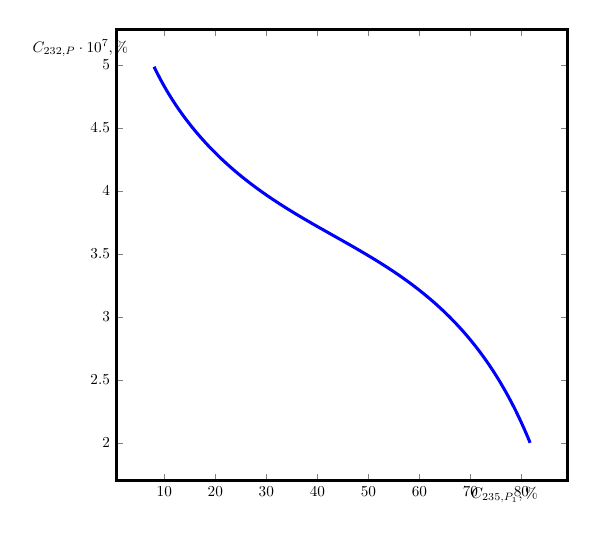
\begin{tikzpicture}[,
scale=0.55]
\begin{axis}[
  xlabel style = {{at={(axis description cs:.86,0)}}},
  ylabel = {$C_{232,P}\cdot10^{7}, \%$},
  ylabel style = {{at={(axis description cs:-0.08,.925)},rotate=270,anchor=south}},
  xlabel = {$C_{235,P_1}, \%$},
  width=12cm, height=12cm, line width=2pt
]

\addplot+[
  mark = {none}
] coordinates {
  (8.0, 4.985973522510448)
  (8.1, 4.977505924459163)
  (8.200000000000001, 4.969120074489785)
  (8.4, 4.95259421778021)
  (8.6, 4.936377217167264)
  (8.9, 4.91261048038541)
  (9.0, 4.904829909624947)
  (9.1, 4.89711636327689)
  (9.2, 4.889470923563254)
  (9.3, 4.881893876682312)
  (9.4, 4.874378735594807)
  (9.5, 4.866927368121624)
  (9.6, 4.859540177519935)
  (9.700000000000001, 4.852212575024995)
  (9.8, 4.844943573960891)
  (9.9, 4.837734018393005)
  (10.0, 4.83058430670322)
  (10.100000000000001, 4.823488916039185)
  (10.2, 4.816449457479848)
  (10.299999999999999, 4.809465627048637)
  (10.4, 4.802534482411325)
  (10.5, 4.795655802947918)
  (10.6, 4.788829583468257)
  (10.7, 4.782053752414381)
  (10.8, 4.7753298626644)
  (10.9, 4.768654370446091)
  (11.0, 4.762027653165846)
  (11.1, 4.755449447960767)
  (11.200000000000001, 4.748914676266442)
  (11.3, 4.742430707255965)
  (11.4, 4.735989990034133)
  (11.5, 4.729594078035632)
  (11.600000000000001, 4.723243289474142)
  (11.700000000000001, 4.7169352940139735)
  (11.799999999999999, 4.710671120806818)
  (11.899999999999999, 4.704448300869189)
  (12.0, 4.698267267895087)
  (12.1, 4.692127765827025)
  (12.2, 4.686028242363314)
  (12.3, 4.67996833795832)
  (12.4, 4.673947210363869)
  (12.5, 4.667970027829537)
  (12.6, 4.6620223620850485)
  (12.7, 4.656116028642911)
  (12.8, 4.650247403238366)
  (12.9, 4.644416172244776)
  (13.0, 4.638621450912494)
  (13.100000000000001, 4.6328618857933614)
  (13.200000000000001, 4.627136824307175)
  (13.3, 4.621446615475064)
  (13.4, 4.615791856559819)
  (13.5, 4.610170473876168)
  (13.600000000000001, 4.604582077783192)
  (13.700000000000001, 4.599027529846763)
  (13.8, 4.5935059909034575)
  (13.900000000000002, 4.588014824269069)
  (14.000000000000002, 4.582557807134732)
  (14.099999999999998, 4.577131597394151)
  (14.2, 4.571736230353866)
  (14.299999999999999, 4.56637059871623)
  (14.399999999999999, 4.561037959480199)
  (14.499999999999998, 4.555733329671543)
  (14.6, 4.550459516090058)
  (14.7, 4.54521417051258)
  (14.799999999999999, 4.539998726671818)
  (14.899999999999999, 4.5348122148974666)
  (15.0, 4.529652927463007)
  (15.1, 4.524524020761017)
  (15.2, 4.519421110774981)
  (15.299999999999999, 4.514347179323051)
  (15.4, 4.509298049967624)
  (15.5, 4.504277703563243)
  (15.6, 4.499282678290834)
  (15.7, 4.494314479772742)
  (15.8, 4.489372620551456)
  (15.9, 4.484456956697928)
  (16.0, 4.479566333442187)
  (16.1, 4.474700999787561)
  (16.2, 4.469861023327496)
  (16.3, 4.465047188482167)
  (16.400000000000002, 4.4602558966412555)
  (16.5, 4.455489183303554)
  (16.6, 4.450747014814206)
  (16.7, 4.446027707669791)
  (16.8, 4.44133333732879)
  (16.900000000000002, 4.43666071815412)
  (17.0, 4.4320115000495495)
  (17.1, 4.42738708381064)
  (17.2, 4.422783108528356)
  (17.299999999999997, 4.418204497049247)
  (17.4, 4.41364580332374)
  (17.5, 4.409108721764048)
  (17.599999999999998, 4.404596207318345)
  (17.7, 4.400102828968469)
  (17.8, 4.395631338040478)
  (17.9, 4.391182147139465)
  (18.0, 4.386754894037566)
  (18.099999999999998, 4.382346257717282)
  (18.2, 4.377961221670567)
  (18.3, 4.3735925508919555)
  (18.4, 4.369247490265301)
  (18.5, 4.36492197401758)
  (18.6, 4.360616190397827)
  (18.7, 4.356332089904171)
  (18.8, 4.352064020151545)
  (18.9, 4.347816740092818)
  (19.0, 4.343590516878981)
  (19.1, 4.339381117555354)
  (19.2, 4.335191894311301)
  (19.3, 4.331023122206472)
  (19.400000000000002, 4.3268714328976605)
  (19.5, 4.32273757802548)
  (19.6, 4.31862215868034)
  (19.7, 4.3145255648029694)
  (19.8, 4.310448349561491)
  (19.900000000000002, 4.306386727999252)
  (20.0, 4.302344458201996)
  (20.1, 4.2983197469929895)
  (20.200000000000003, 4.294311492711422)
  (20.3, 4.290320923173377)
  (20.4, 4.286347917769717)
  (20.5, 4.282392242676548)
  (20.599999999999998, 4.278453866887021)
  (20.7, 4.274532022271439)
  (20.8, 4.2706257911966805)
  (20.9, 4.266737034502461)
  (21.0, 4.262864465960168)
  (21.099999999999998, 4.259009872360633)
  (21.2, 4.255168651065848)
  (21.3, 4.251344713374651)
  (21.4, 4.2475375547498535)
  (21.5, 4.243745715376132)
  (21.6, 4.239968999445669)
  (21.7, 4.236207977564669)
  (21.8, 4.232461512144874)
  (21.9, 4.228731940970158)
  (22.0, 4.225018395232093)
  (22.1, 4.221317399173533)
  (22.2, 4.217633509858051)
  (22.3, 4.213962024137284)
  (22.400000000000002, 4.2103048871508015)
  (22.5, 4.206667104661477)
  (22.6, 4.203041761543867)
  (22.7, 4.199429251238778)
  (22.8, 4.195831893329498)
  (22.900000000000002, 4.192249558553893)
  (23.0, 4.18868081378806)
  (23.1, 4.185125682446771)
  (23.200000000000003, 4.1815846231491065)
  (23.3, 4.178057473628274)
  (23.400000000000002, 4.174543188134159)
  (23.5, 4.171044228031182)
  (23.599999999999998, 4.167556173255368)
  (23.7, 4.1640841418671934)
  (23.799999999999997, 4.1606245488560285)
  (23.9, 4.157178251911083)
  (24.0, 4.153744326065294)
  (24.099999999999998, 4.150324464348545)
  (24.2, 4.146916338742175)
  (24.3, 4.143520537439906)
  (24.4, 4.140139532351757)
  (24.5, 4.136769694305907)
  (24.6, 4.1334118067273)
  (24.7, 4.130068527667547)
  (24.8, 4.126734791016853)
  (24.9, 4.123416091895991)
  (25.0, 4.120108179852417)
  (25.1, 4.11681163164308)
  (25.2, 4.1135286830383135)
  (25.3, 4.110257261421574)
  (25.4, 4.1069976269620705)
  (25.5, 4.103749190826508)
  (25.6, 4.100512973126756)
  (25.7, 4.097286407256865)
  (25.8, 4.0940733773335785)
  (25.900000000000002, 4.090870909796634)
  (26.0, 4.087679138059313)
  (26.1, 4.084499864717345)
  (26.200000000000003, 4.081330653459896)
  (26.3, 4.078174109510021)
  (26.400000000000002, 4.075025872101862)
  (26.5, 4.071891686823192)
  (26.6, 4.068766217961799)
  (26.700000000000003, 4.0656523721540685)
  (26.8, 4.062548541059717)
  (26.900000000000002, 4.059454893767616)
  (27.0, 4.056372420569818)
  (27.1, 4.0532991182147615)
  (27.200000000000003, 4.050237946305979)
  (27.3, 4.047185216196656)
  (27.400000000000002, 4.044143014531759)
  (27.500000000000004, 4.0411135017719335)
  (27.6, 4.03808989041423)
  (27.700000000000003, 4.035078664106977)
  (27.800000000000004, 4.032076980641798)
  (27.900000000000002, 4.029084385290031)
  (28.000000000000004, 4.026102741679855)
  (28.1, 4.023129672257948)
  (28.199999999999996, 4.020167126612971)
  (28.299999999999997, 4.017213730273181)
  (28.4, 4.014267461034477)
  (28.499999999999996, 4.011333769765237)
  (28.599999999999998, 4.008407283113078)
  (28.7, 4.005490550390849)
  (28.799999999999997, 4.002583926708362)
  (28.9, 3.9996849725763273)
  (28.999999999999996, 3.996793639575309)
  (29.099999999999998, 3.9939138365914504)
  (29.2, 3.9910425115295527)
  (29.299999999999997, 3.9881786004707798)
  (29.4, 3.985323788926678)
  (29.5, 3.982478754305616)
  (29.599999999999998, 3.979640802886997)
  (29.7, 3.9768118691535195)
  (29.799999999999997, 3.973990447782564)
  (29.9, 3.97117767405895)
  (30.0, 3.968374078915672)
  (30.099999999999998, 3.965578022196386)
  (30.2, 3.9627906581777794)
  (30.3, 3.960010420461657)
  (30.4, 3.9572384233805007)
  (30.5, 3.954475145658851)
  (30.599999999999998, 3.9517177342551926)
  (30.7, 3.9489688450666725)
  (30.8, 3.9462289208424464)
  (30.9, 3.9434946276150664)
  (31.0, 3.940770415103327)
  (31.1, 3.938051285932105)
  (31.2, 3.935340527555951)
  (31.3, 3.9326359753752302)
  (31.4, 3.929940400536781)
  (31.5, 3.927251833220745)
  (31.6, 3.9245704569608555)
  (31.7, 3.9218946822100746)
  (31.8, 3.9192269949754897)
  (31.900000000000002, 3.916566302978504)
  (32.0, 3.9139120696040175)
  (32.1, 3.911265080978627)
  (32.2, 3.9086245028278044)
  (32.300000000000004, 3.9059914605853834)
  (32.4, 3.9033635456460822)
  (32.5, 3.9007422564291026)
  (32.6, 3.8981281279596374)
  (32.7, 3.8955201573004903)
  (32.800000000000004, 3.892919506686707)
  (32.9, 3.890323781112805)
  (33.0, 3.8877332726176017)
  (33.1, 3.8851522186799734)
  (33.2, 3.882575108308945)
  (33.300000000000004, 3.8800032571833243)
  (33.4, 3.877440046750663)
  (33.5, 3.8748810903455784)
  (33.6, 3.8723281489984704)
  (33.7, 3.869780873657687)
  (33.800000000000004, 3.8672396265557523)
  (33.900000000000006, 3.864702733004999)
  (34.0, 3.8621727558284618)
  (34.1, 3.859648253160404)
  (34.2, 3.8571286109470635)
  (34.300000000000004, 3.8546147410146805)
  (34.4, 3.8521058114793236)
  (34.5, 3.849601675130475)
  (34.599999999999994, 3.847103002597281)
  (34.699999999999996, 3.844611022746586)
  (34.8, 3.842122889056423)
  (34.9, 3.8396406282553484)
  (35.0, 3.8371618735615383)
  (35.099999999999994, 3.8346886940851928)
  (35.199999999999996, 3.8322198343163403)
  (35.3, 3.829756817457991)
  (35.4, 3.8272984222838655)
  (35.5, 3.8248442986617435)
  (35.6, 3.822393875034278)
  (35.699999999999996, 3.819948369774754)
  (35.8, 3.817507857147374)
  (35.9, 3.8150715397535064)
  (36.0, 3.8126396925705137)
  (36.1, 3.8102109844462433)
  (36.199999999999996, 3.8077888536216626)
  (36.3, 3.805368426628278)
  (36.4, 3.8029538963003624)
  (36.5, 3.8005425419853944)
  (36.6, 3.7981332264977183)
  (36.7, 3.7957325903904944)
  (36.8, 3.7933321267969435)
  (36.9, 3.790935048517987)
  (37.0, 3.7885440012654055)
  (37.1, 3.7861549982668348)
  (37.2, 3.7837700806785364)
  (37.3, 3.7813901337392384)
  (37.4, 3.779011688302321)
  (37.5, 3.776637206555999)
  (37.6, 3.77426623330392)
  (37.7, 3.771898135239139)
  (37.8, 3.769533656672267)
  (37.9, 3.767172764247592)
  (38.0, 3.764813977584719)
  (38.1, 3.7624588954409433)
  (38.2, 3.7601067000397417)
  (38.3, 3.75775752789605)
  (38.4, 3.7554110872989517)
  (38.5, 3.753067594777724)
  (38.6, 3.750726730502418)
  (38.7, 3.748388696869003)
  (38.800000000000004, 3.7460522591028194)
  (38.9, 3.743719439222531)
  (39.0, 3.7413888151120913)
  (39.1, 3.7390617444737178)
  (39.2, 3.7367361840983935)
  (39.300000000000004, 3.734413333606388)
  (39.4, 3.7320909201008514)
  (39.5, 3.7297719442210715)
  (39.6, 3.727455590233747)
  (39.7, 3.725140657384657)
  (39.800000000000004, 3.722828772195745)
  (39.900000000000006, 3.720518106189269)
  (40.0, 3.7182092951150993)
  (40.1, 3.715903493080819)
  (40.2, 3.713597564847497)
  (40.300000000000004, 3.711294366629864)
  (40.400000000000006, 3.708991932484848)
  (40.5, 3.7066922635513957)
  (40.6, 3.704393901698177)
  (40.699999999999996, 3.7020970293951785)
  (40.8, 3.699800619521217)
  (40.9, 3.6975070820700964)
  (41.0, 3.6952136043528045)
  (41.099999999999994, 3.6929231167170355)
  (41.199999999999996, 3.6906328792692156)
  (41.3, 3.6883436486964)
  (41.4, 3.6860553106590412)
  (41.5, 3.6837691401299897)
  (41.6, 3.6814824255542677)
  (41.699999999999996, 3.6791968526203997)
  (41.8, 3.6769121510425156)
  (41.9, 3.6746284326273764)
  (42.0, 3.6723454349978173)
  (42.1, 3.67006289163852)
  (42.199999999999996, 3.6677814408255904)
  (42.3, 3.665500331181984)
  (42.4, 3.6632198730616454)
  (42.5, 3.6609400538926726)
  (42.6, 3.6586597313315252)
  (42.699999999999996, 3.656380418131201)
  (42.8, 3.654101167067256)
  (42.9, 3.6518208753364423)
  (43.0, 3.6495417721846897)
  (43.1, 3.647263227683627)
  (43.2, 3.644984716137399)
  (43.3, 3.642706146036691)
  (43.4, 3.6404260694191892)
  (43.5, 3.638146380104459)
  (43.6, 3.6358680043028055)
  (43.7, 3.633588257651532)
  (43.8, 3.6313081242428558)
  (43.9, 3.6290281788521805)
  (44.0, 3.626746206586419)
  (44.1, 3.6244644603004295)
  (44.2, 3.6221830519188383)
  (44.3, 3.6199003140514177)
  (44.4, 3.6176176407356193)
  (44.5, 3.615332070424727)
  (44.6, 3.6130469816150566)
  (44.7, 3.610761338811265)
  (44.800000000000004, 3.6084746786929363)
  (44.9, 3.606187875125979)
  (45.0, 3.6038972174062134)
  (45.1, 3.60160700032948)
  (45.2, 3.5993165808145795)
  (45.300000000000004, 3.597023443595911)
  (45.4, 3.5947293263166795)
  (45.5, 3.592433613457347)
  (45.6, 3.5901375440153553)
  (45.7, 3.587838830550874)
  (45.800000000000004, 3.585539589446617)
  (45.9, 3.58323760760154)
  (46.0, 3.5809338977683267)
  (46.1, 3.5786297754681606)
  (46.2, 3.5763242516376557)
  (46.300000000000004, 3.574015345862727)
  (46.400000000000006, 3.5717045142148693)
  (46.5, 3.5693935957291774)
  (46.6, 3.567078245758539)
  (46.7, 3.564762354210005)
  (46.800000000000004, 3.5624434042320816)
  (46.9, 3.560123048030059)
  (47.0, 3.55779926557382)
  (47.099999999999994, 3.555473856733785)
  (47.199999999999996, 3.553146398275374)
  (47.3, 3.5508159053216715)
  (47.4, 3.5484823105295122)
  (47.5, 3.5461475198493044)
  (47.599999999999994, 3.5438102181520095)
  (47.699999999999996, 3.5414686970508282)
  (47.8, 3.5391244006206053)
  (47.9, 3.5367782598572486)
  (48.0, 3.5344286752951537)
  (48.1, 3.532076848188982)
  (48.199999999999996, 3.5297217695142167)
  (48.3, 3.527363781795185)
  (48.4, 3.525001712431128)
  (48.5, 3.5226369818909573)
  (48.6, 3.520269337068263)
  (48.699999999999996, 3.5178978386086697)
  (48.8, 3.515523829533761)
  (48.9, 3.5131454840380507)
  (49.0, 3.510764427930477)
  (49.1, 3.5083794761169016)
  (49.2, 3.505990324905092)
  (49.3, 3.50359797832314)
  (49.4, 3.501201667797517)
  (49.5, 3.498801876668478)
  (49.6, 3.4963969439234064)
  (49.7, 3.4939902283376583)
  (49.8, 3.4915780714170275)
  (49.9, 3.489162097185752)
  (50.0, 3.486741683696293)
  (50.1, 3.4843175093301366)
  (50.2, 3.4818888989266625)
  (50.3, 3.4794560168307873)
  (50.4, 3.4770187509384574)
  (50.5, 3.4745770676667584)
  (50.6, 3.472130757433451)
  (50.7, 3.4696798665005226)
  (50.8, 3.467224389177408)
  (50.9, 3.464763188431182)
  (51.0, 3.462298880038757)
  (51.1, 3.4598281513175895)
  (51.2, 3.4573538268466955)
  (51.300000000000004, 3.4548736377062763)
  (51.4, 3.4523889238922387)
  (51.5, 3.4498993230864707)
  (51.6, 3.4474055109185078)
  (51.7, 3.4449035879646925)
  (51.800000000000004, 3.442398385755517)
  (51.9, 3.4398880804299075)
  (52.0, 3.4373712065623816)
  (52.1, 3.4348497585510405)
  (52.2, 3.4323213942272535)
  (52.300000000000004, 3.429788996276968)
  (52.400000000000006, 3.4272501232779553)
  (52.5, 3.4247049723798266)
  (52.6, 3.4221551390210925)
  (52.7, 3.4196003029509634)
  (52.800000000000004, 3.4170366975933826)
  (52.900000000000006, 3.4144689018000354)
  (53.0, 3.411894328742276)
  (53.1, 3.4093131041588456)
  (53.2, 3.4067274494116515)
  (53.300000000000004, 3.4041331689588494)
  (53.400000000000006, 3.4015354262530257)
  (53.5, 3.3989270061827237)
  (53.6, 3.396314846037327)
  (53.7, 3.393696226939984)
  (53.800000000000004, 3.391072753741774)
  (53.900000000000006, 3.3884386459092455)
  (54.0, 3.385799023602791)
  (54.1, 3.383153581748245)
  (54.2, 3.380501074567424)
  (54.300000000000004, 3.3778404548576275)
  (54.400000000000006, 3.375172380138389)
  (54.50000000000001, 3.372500275236679)
  (54.6, 3.3698185236781835)
  (54.7, 3.367129379705533)
  (54.800000000000004, 3.3644348941081925)
  (54.900000000000006, 3.361731711747348)
  (55.00000000000001, 3.3590208212707506)
  (55.1, 3.3563012294354704)
  (55.2, 3.353575171425897)
  (55.300000000000004, 3.3508412147372826)
  (55.400000000000006, 3.348099974865795)
  (55.50000000000001, 3.3453509061680404)
  (55.60000000000001, 3.3425941488643303)
  (55.7, 3.339829619391547)
  (55.800000000000004, 3.337055296418172)
  (55.900000000000006, 3.3342741049349693)
  (56.00000000000001, 3.3314843120486404)
  (56.10000000000001, 3.3286876362204025)
  (56.2, 3.325880775132288)
  (56.3, 3.32306554848977)
  (56.39999999999999, 3.320241892318642)
  (56.49999999999999, 3.3174108259230493)
  (56.599999999999994, 3.3145697557970046)
  (56.699999999999996, 3.3117212020413143)
  (56.8, 3.3088621609567226)
  (56.89999999999999, 3.305995801897854)
  (56.99999999999999, 3.3031201434396706)
  (57.099999999999994, 3.300234712736228)
  (57.199999999999996, 3.2973407374824295)
  (57.3, 3.2944370778064074)
  (57.4, 3.2915254598178074)
  (57.49999999999999, 3.28860292898421)
  (57.599999999999994, 3.2856717362787276)
  (57.699999999999996, 3.2827312751672824)
  (57.8, 3.2797798809666583)
  (57.9, 3.2768201416612666)
  (57.99999999999999, 3.2738507197167546)
  (58.099999999999994, 3.2708707204722307)
  (58.199999999999996, 3.2678807655052204)
  (58.3, 3.264880366868151)
  (58.4, 3.2618712103079988)
  (58.5, 3.2588513330233058)
  (58.599999999999994, 3.2558223888536246)
  (58.699999999999996, 3.2527810297164055)
  (58.8, 3.2497297823929525)
  (58.9, 3.2466680466273883)
  (59.0, 3.2435966294753538)
  (59.099999999999994, 3.2405141383424967)
  (59.199999999999996, 3.2374207427985207)
  (59.3, 3.234316765642639)
  (59.4, 3.231200930766104)
  (59.5, 3.2280743183294494)
  (59.599999999999994, 3.224937482458711)
  (59.699999999999996, 3.221788135183967)
  (59.8, 3.2186294523539445)
  (59.9, 3.215459212202454)
  (60.0, 3.212276938587741)
  (60.099999999999994, 3.209082732765658)
  (60.199999999999996, 3.2058770380036434)
  (60.3, 3.202660629459712)
  (60.4, 3.199429805686613)
  (60.5, 3.1961887966942033)
  (60.6, 3.192937348222832)
  (60.699999999999996, 3.1896710299269255)
  (60.8, 3.1863945062625567)
  (60.9, 3.1831045516318217)
  (61.0, 3.1798014898631823)
  (61.1, 3.176488920811933)
  (61.199999999999996, 3.1731618369606283)
  (61.3, 3.1698221544554364)
  (61.4, 3.166470594039824)
  (61.5, 3.1631055458507675)
  (61.6, 3.1597272697800824)
  (61.7, 3.156336248676202)
  (61.8, 3.1529327486880385)
  (61.9, 3.1495143467930284)
  (62.0, 3.1460834458599334)
  (62.1, 3.1426380975065613)
  (62.2, 3.1391817966626108)
  (62.3, 3.1357099247505693)
  (62.4, 3.1322258915303935)
  (62.5, 3.128726995181226)
  (62.6, 3.1252140427476203)
  (62.7, 3.1216871630087324)
  (62.8, 3.118145449009835)
  (62.9, 3.1145911141747753)
  (63.0, 3.1110208426882626)
  (63.1, 3.107436925903713)
  (63.2, 3.1038382568248477)
  (63.3, 3.1002246655742667)
  (63.4, 3.096597433082471)
  (63.5, 3.0929537575809496)
  (63.6, 3.0892965392082754)
  (63.7, 3.0856231655806305)
  (63.800000000000004, 3.0819349756277132)
  (63.9, 3.0782309191047)
  (64.0, 3.074511838339552)
  (64.1, 3.070776203309121)
  (64.2, 3.0670268348314833)
  (64.3, 3.063259611674829)
  (64.4, 3.0594774928420296)
  (64.5, 3.055679384334054)
  (64.60000000000001, 3.051864771331426)
  (64.7, 3.0480341322095397)
  (64.8, 3.0441868117763407)
  (64.9, 3.0403229605342617)
  (65.0, 3.0364432061676725)
  (65.10000000000001, 3.032545370519572)
  (65.2, 3.028631372831375)
  (65.3, 3.024699723206217)
  (65.4, 3.0207517454923156)
  (65.5, 3.0167861891416683)
  (65.60000000000001, 3.012801399176915)
  (65.7, 3.0088017989124967)
  (65.8, 3.004783162098373)
  (65.9, 3.0007467779886534)
  (66.0, 2.996693367447261)
  (66.10000000000001, 2.992620533702903)
  (66.2, 2.9885301233541024)
  (66.3, 2.984420470611333)
  (66.4, 2.980293148112526)
  (66.5, 2.976147372650165)
  (66.60000000000001, 2.971983386111706)
  (66.7, 2.967798618812177)
  (66.8, 2.9635969985739536)
  (66.9, 2.959374383449302)
  (67.0, 2.95513262813881)
  (67.10000000000001, 2.950872316303311)
  (67.2, 2.9465906261137076)
  (67.30000000000001, 2.942291674117397)
  (67.4, 2.9379706038886844)
  (67.5, 2.933628956936002)
  (67.60000000000001, 2.9292683153093653)
  (67.7, 2.9248877485187164)
  (67.80000000000001, 2.920485392711807)
  (67.9, 2.9160620576918883)
  (68.0, 2.9116189086195288)
  (68.10000000000001, 2.9071546425104446)
  (68.2, 2.9026675301038134)
  (68.30000000000001, 2.898160563270578)
  (68.4, 2.893633173332283)
  (68.5, 2.88908276566014)
  (68.60000000000001, 2.884508416929432)
  (68.7, 2.8799136189672443)
  (68.8, 2.8752966263553312)
  (68.89999999999999, 2.8706592974092198)
  (69.0, 2.8659966086698527)
  (69.1, 2.861312154677081)
  (69.19999999999999, 2.856603462877766)
  (69.3, 2.851872791953686)
  (69.39999999999999, 2.8471192655633955)
  (69.5, 2.842341252018293)
  (69.6, 2.8375409072738695)
  (69.69999999999999, 2.8327143893265823)
  (69.8, 2.8278647115128424)
  (69.89999999999999, 2.8229913014368284)
  (70.0, 2.818092354405924)
  (70.1, 2.8131699715222442)
  (70.19999999999999, 2.8082218803030004)
  (70.3, 2.8032497901612823)
  (70.39999999999999, 2.798252691049421)
  (70.5, 2.793229711269239)
  (70.6, 2.7881787088043533)
  (70.7, 2.7831046494597125)
  (70.8, 2.778004088304338)
  (70.89999999999999, 2.772875826403187)
  (71.0, 2.767722679162932)
  (71.1, 2.7625420155454523)
  (71.2, 2.757334380488374)
  (71.3, 2.752099721489052)
  (71.39999999999999, 2.7468376266295214)
  (71.5, 2.7415476435064488)
  (71.6, 2.736230025584535)
  (71.7, 2.730885226343742)
  (71.8, 2.7255110120477104)
  (71.89999999999999, 2.720109700579866)
  (72.0, 2.7146773533714077)
  (72.1, 2.70921752772082)
  (72.2, 2.703727701802331)
  (72.3, 2.698208959060878)
  (72.39999999999999, 2.6926593514181105)
  (72.5, 2.68708171313301)
  (72.6, 2.681472674326306)
  (72.7, 2.6758337945535464)
  (72.8, 2.6701628281855108)
  (72.89999999999999, 2.6644621171923406)
  (73.0, 2.6587293176769506)
  (73.1, 2.6529661308605106)
  (73.2, 2.647170190271161)
  (73.3, 2.641342034538594)
  (73.4, 2.6354850857625296)
  (73.5, 2.629591678978951)
  (73.6, 2.623663574477364)
  (73.7, 2.6177051401593046)
  (73.8, 2.611713035432089)
  (73.9, 2.6056866163382812)
  (74.0, 2.5996267177539396)
  (74.1, 2.593532075401762)
  (74.2, 2.587404600786781)
  (74.3, 2.5812403685847585)
  (74.4, 2.5750408951518904)
  (74.5, 2.568806247626845)
  (74.6, 2.5625354652837866)
  (74.7, 2.5562288970697993)
  (74.8, 2.5498881855718367)
  (74.9, 2.5435080765064604)
  (75.0, 2.537090646969461)
  (75.1, 2.530636603112387)
  (75.2, 2.5241448500066386)
  (75.3, 2.5176147832151083)
  (75.4, 2.5110468883789747)
  (75.5, 2.504440475342071)
  (75.6, 2.497794087549945)
  (75.7, 2.4911084577476323)
  (75.8, 2.4843834690758118)
  (75.9, 2.477617557946219)
  (76.0, 2.470812500392288)
  (76.1, 2.4639657227267637)
  (76.2, 2.4570780693793153)
  (76.3, 2.4501479640786576)
  (76.4, 2.4431764129710265)
  (76.5, 2.4361628019416988)
  (76.6, 2.4291063280135856)
  (76.7, 2.422006678237375)
  (76.8, 2.4148636370828727)
  (76.9, 2.407676040537025)
  (77.0, 2.4004442499532583)
  (77.10000000000001, 2.3931673610309416)
  (77.2, 2.3858471761679114)
  (77.3, 2.3784813356506507)
  (77.4, 2.3710668082226025)
  (77.5, 2.3636081989622006)
  (77.60000000000001, 2.3561006927626362)
  (77.7, 2.3485474531025945)
  (77.8, 2.3409476997613994)
  (77.9, 2.3332969689619096)
  (78.0, 2.3255986833446594)
  (78.10000000000001, 2.3178507948774154)
  (78.2, 2.310053286769979)
  (78.3, 2.3022054473042)
  (78.4, 2.2943068617055586)
  (78.5, 2.2863575790881367)
  (78.60000000000001, 2.278356675508693)
  (78.7, 2.2703036075616887)
  (78.8, 2.262197357061142)
  (78.9, 2.2540388433458327)
  (79.0, 2.2458240962575506)
  (79.10000000000001, 2.2375565001214706)
  (79.2, 2.2292342803495098)
  (79.3, 2.22085529272664)
  (79.4, 2.212420979156209)
  (79.5, 2.2039301085231067)
  (79.60000000000001, 2.1953810428266523)
  (79.7, 2.1867738774261087)
  (79.80000000000001, 2.178108251568322)
  (79.9, 2.1693838834679586)
  (80.0, 2.1606031967894173)
  (80.10000000000001, 2.1517537637757482)
  (80.2, 2.1428468366637357)
  (80.30000000000001, 2.1338783681076783)
  (80.4, 2.124846043474167)
  (80.5, 2.115750353449903)
  (80.60000000000001, 2.1065906985623966)
  (80.7, 2.097365518939154)
  (80.80000000000001, 2.088075128510556)
  (80.9, 2.0787180058229704)
  (81.0, 2.0692932452946926)
  (81.10000000000001, 2.0597998378944413)
  (81.2, 2.0502378752073325)
  (81.3, 2.0406059961159064)
  (81.39999999999999, 2.0309015529503838)
  (81.5, 2.0211276212760936)
  (81.6, 2.011279839931154)
  (81.69999999999999, 2.001356762565841)
};

\end{axis}
\end{tikzpicture}


    \caption{{Зависимость концентрации $^{232}$U в потоке НОУ-продукта от концентрации $^{235}$U в потоке легкой фракции первого каскада ($P_1$){\label{C232P}}}}
  \end{minipage}%
  \begin{minipage}{.5\textwidth}
    \centering
    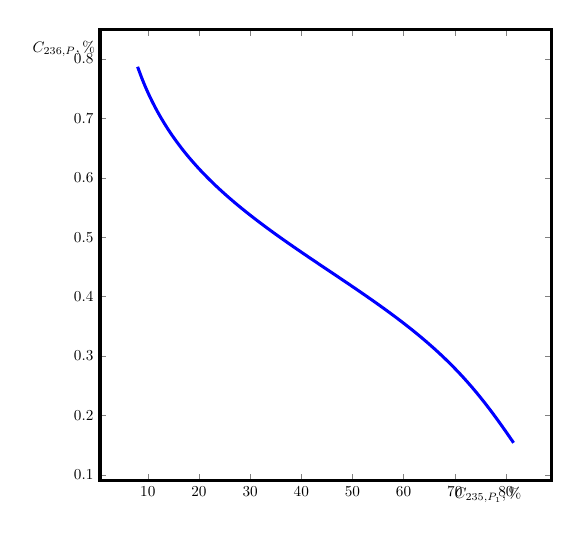
\begin{tikzpicture}[,
scale=0.55]
\begin{axis}[
  xlabel style = {{at={(axis description cs:.86,0)}}},
  ylabel = {$C_{236,P}, \%$},
  ylabel style = {{at={(axis description cs:-0.08,.925)},rotate=270,anchor=south}},
  xlabel = {$C_{235,P_1}, \%$},
  width=12cm, height=12cm, line width=2pt
]

\addplot+[
  mark = {none}
] coordinates {
  (8.0, 0.7868682760670866)
  (8.75, 0.7694398277179685)
  (9.0, 0.7640109280998006)
  (9.25, 0.7587520475138675)
  (9.5, 0.7536526588806822)
  (9.75, 0.7487031554326434)
  (10.0, 0.743894742047762)
  (10.25, 0.7392193471528742)
  (10.5, 0.7346695568041786)
  (10.75, 0.7302385309442729)
  (11.0, 0.7259199568471547)
  (11.25, 0.7217079942160229)
  (11.5, 0.7175972289868053)
  (11.75, 0.7135826346256019)
  (12.0, 0.7096595332400356)
  (12.25, 0.7058235688816951)
  (12.5, 0.7020706791285567)
  (12.75, 0.6983970597638589)
  (13.0, 0.694799157335174)
  (13.25, 0.691273639735873)
  (13.5, 0.6878173738461844)
  (13.750000000000002, 0.684427444003394)
  (14.000000000000002, 0.6811010637602548)
  (14.249999999999998, 0.6778356381461185)
  (14.499999999999998, 0.6746287140566715)
  (14.75, 0.6714779722338093)
  (15.0, 0.668381227607892)
  (15.25, 0.6653364097634284)
  (15.5, 0.66234155660075)
  (15.75, 0.6593948110703204)
  (16.0, 0.656494409200412)
  (16.25, 0.6536386804288195)
  (16.5, 0.6508260340255825)
  (16.75, 0.6480549570845349)
  (17.0, 0.6453240099696453)
  (17.25, 0.6426318244316405)
  (17.5, 0.6399770888968725)
  (17.75, 0.6373585602180389)
  (18.0, 0.6347750461866616)
  (18.25, 0.6322254086937356)
  (18.5, 0.6297085604431246)
  (18.75, 0.6272234605491067)
  (19.0, 0.6247691152458444)
  (19.25, 0.6223445699476854)
  (19.5, 0.6199489060744346)
  (19.75, 0.6175812460815923)
  (20.0, 0.6152407525309614)
  (20.25, 0.6129266131916922)
  (20.5, 0.6106380529837465)
  (20.75, 0.6083743239726872)
  (21.0, 0.6061347079619203)
  (21.25, 0.6039185130158939)
  (21.5, 0.6017250707244296)
  (21.75, 0.5995537447209317)
  (22.0, 0.5974039148632175)
  (22.25, 0.5952749816498157)
  (22.5, 0.5931663751875551)
  (22.75, 0.5910775353950994)
  (23.0, 0.5890079281004936)
  (23.25, 0.5869570332614675)
  (23.5, 0.5849243515350462)
  (23.75, 0.5829093972592186)
  (24.0, 0.5809117008875728)
  (24.25, 0.5789308094893011)
  (24.5, 0.576966285159205)
  (24.75, 0.5750177035056347)
  (25.0, 0.5730846414739709)
  (25.25, 0.5711667111048804)
  (25.5, 0.5692635184939031)
  (25.75, 0.5673746882002044)
  (26.0, 0.5654998548903026)
  (26.25, 0.5636386643667142)
  (26.5, 0.5617907706950359)
  (26.75, 0.5599558375776155)
  (27.0, 0.5581335409114757)
  (27.250000000000004, 0.5563235621499162)
  (27.500000000000004, 0.5545255950371053)
  (27.750000000000004, 0.5527393362732191)
  (28.000000000000004, 0.5509644954034985)
  (28.249999999999996, 0.5492007879150705)
  (28.499999999999996, 0.5474479351694349)
  (28.749999999999996, 0.5457056663039109)
  (28.999999999999996, 0.5439737179602749)
  (29.25, 0.542251834590858)
  (29.5, 0.5405397629597792)
  (29.75, 0.5388372579816432)
  (30.0, 0.5371440796437678)
  (30.25, 0.535459995439975)
  (30.5, 0.5337847763003427)
  (30.75, 0.5321181968409991)
  (31.0, 0.5304600414608782)
  (31.25, 0.5288100933491828)
  (31.5, 0.527168145175653)
  (31.75, 0.5255339900302419)
  (32.0, 0.5239074304973325)
  (32.25, 0.5222882668838474)
  (32.5, 0.5206763065687176)
  (32.75, 0.519071362983488)
  (33.0, 0.5174732457017434)
  (33.25, 0.5158817796161442)
  (33.5, 0.5142967815840024)
  (33.75, 0.5127180769972177)
  (34.0, 0.511145494693123)
  (34.25, 0.5095788645943036)
  (34.5, 0.508018019889726)
  (34.75, 0.5064628000631314)
  (35.0, 0.5049130402679127)
  (35.25, 0.5033685854636027)
  (35.5, 0.5018292775341852)
  (35.75, 0.5002949641009634)
  (36.0, 0.49876549368959056)
  (36.25, 0.4972407179731142)
  (36.5, 0.495720489584218)
  (36.75, 0.49420466337566393)
  (37.0, 0.49269309768507813)
  (37.25, 0.49118565095023997)
  (37.5, 0.4896821828212602)
  (37.75, 0.488182557123299)
  (38.0, 0.4866866374862446)
  (38.25, 0.48519429016161053)
  (38.5, 0.48370538081133524)
  (38.75, 0.4822197790527591)
  (39.0, 0.4807373547027698)
  (39.25, 0.47925797948041704)
  (39.5, 0.47778152561950665)
  (39.75, 0.4763078672114897)
  (40.0, 0.47483687793343804)
  (40.25, 0.47336843372565934)
  (40.5, 0.47190241152472157)
  (40.75, 0.4704386902575177)
  (41.0, 0.4689771451341304)
  (41.25, 0.46751766159381897)
  (41.5, 0.46606011474593934)
  (41.75, 0.464604386522142)
  (42.0, 0.4631503589702256)
  (42.25, 0.46169791511084457)
  (42.5, 0.46024693686925977)
  (42.75, 0.4587973075959438)
  (43.0, 0.4573489100330952)
  (43.25, 0.4559016312317238)
  (43.5, 0.4544553520760873)
  (43.75, 0.45300996105426383)
  (44.0, 0.4515653403282681)
  (44.25, 0.45012137645243855)
  (44.5, 0.4486779553788292)
  (44.75, 0.447234961381956)
  (45.0, 0.4457922811936875)
  (45.25, 0.44434980037979505)
  (45.5, 0.4429074034604019)
  (45.75, 0.44146497803251816)
  (46.0, 0.4400224072375789)
  (46.25, 0.43857958086136645)
  (46.5, 0.43713637942272904)
  (46.75, 0.43569268773539566)
  (47.0, 0.4342483946246159)
  (47.25, 0.4328033810238779)
  (47.5, 0.43135753251519143)
  (47.75, 0.4299107582431485)
  (48.0, 0.4284628893033023)
  (48.25, 0.4270138367332666)
  (48.5, 0.4255634759677994)
  (48.75, 0.42411169490214323)
  (49.0, 0.42265836932761647)
  (49.25, 0.4212033812745981)
  (49.5, 0.41974661029222404)
  (49.75, 0.41828793352223503)
  (50.0, 0.4168272285498969)
  (50.24999999999999, 0.41536437261279646)
  (50.5, 0.41389924092878433)
  (50.74999999999999, 0.4124317079453899)
  (51.0, 0.4109616463817828)
  (51.24999999999999, 0.409488929327514)
  (51.5, 0.40801342806205465)
  (51.74999999999999, 0.40653501254219)
  (52.0, 0.4050535510141912)
  (52.25, 0.4035689096851132)
  (52.5, 0.4020809570541411)
  (52.75, 0.4005895561136774)
  (53.0, 0.39909456936941706)
  (53.25, 0.39759586168480915)
  (53.5, 0.39609327971331576)
  (53.75, 0.3945866973437146)
  (54.0, 0.39307596321178706)
  (54.25, 0.39156093398960146)
  (54.50000000000001, 0.3900414609762124)
  (54.75, 0.3885173941988575)
  (55.00000000000001, 0.38698858223635374)
  (55.25, 0.38545487067247325)
  (55.50000000000001, 0.38391610649080016)
  (55.75, 0.38237213035191997)
  (56.00000000000001, 0.3808227801906791)
  (56.25, 0.37926789500729247)
  (56.49999999999999, 0.3777073110034429)
  (56.75, 0.37614085823178506)
  (56.99999999999999, 0.3745683665518605)
  (57.25, 0.37298966300023106)
  (57.49999999999999, 0.37140457391164944)
  (57.75, 0.3698129197055191)
  (57.99999999999999, 0.3682145189898214)
  (58.25, 0.3666091847541619)
  (58.5, 0.3649967355850552)
  (58.75, 0.3633769779054105)
  (59.0, 0.3617497167136132)
  (59.25, 0.3601147568629273)
  (59.5, 0.35847189584694916)
  (59.75, 0.3568209343772881)
  (60.0, 0.35516166110706804)
  (60.25, 0.35349386636535757)
  (60.5, 0.35181733486293343)
  (60.75000000000001, 0.3501318523427276)
  (61.0, 0.34843718912909877)
  (61.25000000000001, 0.3467331282750314)
  (61.5, 0.3450194355029112)
  (61.75000000000001, 0.34329587496967395)
  (62.0, 0.34156221117256785)
  (62.25000000000001, 0.33981820178357364)
  (62.5, 0.3380636015637099)
  (62.74999999999999, 0.33629815736821317)
  (63.0, 0.3345216155346443)
  (63.24999999999999, 0.332733718292191)
  (63.5, 0.33093420053544037)
  (63.74999999999999, 0.32912279575736897)
  (64.0, 0.32729922985126547)
  (64.25, 0.3254632272761041)
  (64.5, 0.32361450660223445)
  (64.75, 0.3217527829601091)
  (65.0, 0.3198777660762714)
  (65.25, 0.317989159835777)
  (65.5, 0.3160866720890013)
  (65.75, 0.31416999507702653)
  (66.0, 0.3122388227099936)
  (66.25, 0.3102928482453305)
  (66.5, 0.3083317514973432)
  (66.75, 0.3063552220516779)
  (67.0, 0.30436293408991816)
  (67.25, 0.302354566254891)
  (67.5, 0.3003297876287052)
  (67.75, 0.29828827488635834)
  (68.0, 0.2962296891835057)
  (68.25, 0.2941537022609022)
  (68.5, 0.2920599797136622)
  (68.75, 0.2899481795919081)
  (69.0, 0.2878179726026076)
  (69.25, 0.2856690203216979)
  (69.5, 0.283500986206298)
  (69.75, 0.281313538246998)
  (70.0, 0.2791063469817097)
  (70.25, 0.27687908456677773)
  (70.5, 0.27463142806318225)
  (70.75, 0.27236305450029297)
  (71.0, 0.27007365796740096)
  (71.25, 0.26776293032395226)
  (71.5, 0.26543057550718885)
  (71.75, 0.2630763099878882)
  (72.0, 0.2606998563422321)
  (72.25, 0.2583009537834834)
  (72.5, 0.25587935596622136)
  (72.75, 0.2534348279069523)
  (73.0, 0.2509671603349918)
  (73.25, 0.24847615690695957)
  (73.5, 0.24596164650198993)
  (73.75, 0.24342347098191244)
  (74.0, 0.2408615142306825)
  (74.25, 0.23827567570941)
  (74.5, 0.23566588781742862)
  (74.75, 0.2330321113551457)
  (75.0, 0.23037434159247525)
  (75.25, 0.22769260868238053)
  (75.5, 0.22498697936797646)
  (75.75, 0.22225755684917442)
  (76.0, 0.21950448585459212)
  (76.25, 0.2167279510285564)
  (76.5, 0.2139281834699162)
  (76.75, 0.21110545134904188)
  (77.0, 0.20826007436313904)
  (77.25, 0.20539241062491168)
  (77.5, 0.20250286778129337)
  (77.75, 0.19959189168573818)
  (78.0, 0.19665998494617906)
  (78.25, 0.19370768674987104)
  (78.5, 0.1907355697280167)
  (78.75, 0.18774426110416553)
  (79.0, 0.1847344125037073)
  (79.25, 0.18170673530355924)
  (79.5, 0.17866195173715402)
  (79.75, 0.1756008411902414)
  (80.0, 0.1725241709493309)
  (80.25, 0.16943273815366058)
  (80.5, 0.1663273960860262)
  (80.75, 0.1632089620925987)
  (81.0, 0.16007831695707048)
  (81.25, 0.15693630120757274)
  (81.5, 0.15378377067086213)
};

\end{axis}
\end{tikzpicture}


    \caption{{Зависимость концентрации $^{236}$U в потоке НОУ-продукта от концентрации $^{235}$U в потоке легкой фракции первого каскада ($P_1$){\label{C236P}}}}
\end{minipage}
\end{figure}


Удельные затраты работы разделения
Перерасход работы разделения
Удельный расход природного урана
Экономия природного урана
Концентрации изотопа $^{235}$U в потоках $W_2$ и $P_0$
Концентраций изотопа $^{236}$U в потоках $W_2$ и $P_1$
Степень извлечения $^{235}$U в первом каскаде
Масса $^{235}$U в потоке $W_2$
Масса $^{235}$U в потоке $P_2$


На рис. \ref{SW_l}-\ref{Fnu} представлены зависимости удельных затрат работы разделения и расхода природного урана, а также величин экономии (перерасхода) для каждой из характеристик по отношению к случаю открытого топливного цикла при тех же внешних условиях. Из анализа представленных кривых видно, что величины расхода природного урана и затрат работы разделения имеют минимум в зависимости от концентрации $C_{235,{P_1}}$. Причём положения этих минимумов различны. Для ответа на вопрос об их появлении рассмотрим рисунки ..., на которых представлены зависимости концентраций изотопа $^{235}$U в потоках $W_2$ и $P_0$, а также концентраций изотопа $^{236}$U в потоках $W_2$ и $P_1$ от величины концентрации $^{235}$U в потоке $P_1$. Анализ представленных зависимостей показывает, что с ростом концентрации $^{235}$U в отборе первого каскада концентрация $^{236}$U ведёт себя немонотонно, достигая максимума при значении концентрации $C_{235,{P_1}}$ приблизительно 60\%. Это обусловлено тем, что с ростом концентрации $^{235}$U в потоке $P_1$ происходит снижение интенсивности обогащения $^{236}$U за счет более интенсивного обогащения более лёгких изотопов $^{232}$U, $^{234}$U. С другой стороны происходит и постепенное уменьшение извлечения $^{235}$U в этот поток. Последний факт подтверждает рис. ..., на котором представлена зависимость степени извлечения $^{235}$U в поток $P_1$. При этом извлечённая в потоке $P_1$ масса $^{235}$U по-разному распределяется между выходящими потоками каскада II (см. рисунки ...). С ростом концентрации $C_{235,{P_1}}$ происходит сокращение обогатительной части каскада II, что неминуемо приводит к росту величины самого потока $P_2$ по отношению к $P_1$ и $W_2$. В результате  в зависимостях массы $^{235}$U в каждом из потоков есть максимум и минимум, совпадающие по положению (см. рис. ...).
При этом максимальной массе $^{235}$U в потоке $W_2$, который участвует в формировании конечного продукта, соответствует минимум величины затрат работы разделения (см. рис. \ref{SW_l}).

Анализ кривой расхода природного урана в зависимости от концентрации изотопа $^{235}$U в отборе первого каскада показывает, что данная величина также имеет минимум, но достигаемый при другом значении концентрации в отборе первого каскада (рис. ...). Возможное объяснение состоит в том, что расход природного урана в схеме полностью определяется каскадом, нарабатывающим НОУ-разбавитель, а также неопределенностью в его параметрах, которые, в свою очередь, зависят от величины добавочного обогащения для компенсации влияния $^{236}$U. Это утверждение иллюстрируют кривые концентрации $^{236}$U в потоке $W_2$ и концентрации $^{236}$U в разбавителе в зависимости от $C_{235,{P_1}}$. Как видно из рис. \ref{C236W2} концентрация $^{236}$U в потоке $W_2$ имеет максимум в зависимости от концентрации $C_{235,{P_1}}$. При этом максимальное значение концентрации $^{236}$U в потоке $W_2$ приблизительно соответствует точке минимуму концентрации $C_{235,{P_0}}$. 

Таким образом, с ростом концентрации изотопа $^{235}$U в отборе первого каскада наблюдается рост концентрации этого же изотопа в потоке $W_2$, что делает возможным понижение концентрации в разбавителе, по-видимому, до того момента, пока масса $^{235}$U в потоке отвала второго каскада не становится настолько малой, что несмотря на рост концентрации данного изотопа, его не хватает по массе и, следовательно, необходимо поднимать его концентрацию в $P_0$.






\subsection{Выводы по результатам исследования эффективности схемы модифицированного двойного каскада}


По результатам анализа представленных решений (табл. \ref{2opt1}--\ref{2opt5_90}) можно сделать следующие выводы:
\begin{itemize}
    \item при отсутствии ограничения на обогащение урановой смеси по $^{235}$U до уровня ВОУ, можно получить финальный продукт со значительно более низкой концентрацией изотопа $^{236}$U, при этом используя НОУ-разбавитель с меньшей концентрацией $^{235}$U, которая не будет выше 5\%;
    \item меньшая концентрация $^{235}$U в легкой фракции первого каскада приводит к необходимости использовать НОУ-разбавитель с более высоким содержанием $^{235}$U, для того чтобы добиться требуемой концентрации $^{235}$U в конечном продукте, что приводит к большему расходу незагрязненного четными изотопами сырьевого материала. При этом, при ограничении на обогащение $^{235}$U в 20\% оптимальные по извлечению $^{235}$U из регенерата решения соответствуют минимально заданной (5\%) концентрации в $P_1$;
    \item для загрязненного четными изотопами состава регенерата (в рассматриваем случае -- состава №2) в процессе оптимизации работы разделения могут быть найдены в качестве оптимальных такие решения, при которых оптимум работы разделения будет достигнут за счет наработки НОУ-продукта по большей части за счет сырья, не содержащего четные изотопы. Поэтому особенно важно контролировать показатель извлечения ценного изотопа $^{235}$U из возвращаемого в цикл регенерата;
    \item отсутствие ограничения в 20\% на обогащение $^{235}$U в каскадной схемы, позволяет улучшить все целевые критерии за счет эффективного концентрирования изотопов $^{236}$U в потоке $P_2$, выводимом из системы. Для этих случаев, по сравнению со случаем, который отличается необходимостью выдерживать ограничение в 20\%, в $P_2$ оказывается меньшее количество изотопа $^{235}$U за счет уменьшения массы потока $P_2$ на 2 порядка. 
\end{itemize}


\section{Анализ <<устойчивости>> предложенного подхода обогащения регенерата к изменению внешних условий}
\subsection{Анализ влияния ограничений предельно допустимой концентрации $^{232}$U в товарном НОУ}

Рассмотренные в предыдущих разделах примеры обогащения регенерированного урана использовали ограничения на концентрации чётных изотопов в товарном НОУ и соотношение между потоками исходного регенерата и конечного продукта, соответствующие требованиям действующих нормативных документов или приведенным в литературе по теме работы \cite{smirnovKaskadnyeShemyZadachah2012}. Очевидно, что выбранные величины могут оказаться другими в будущем. То же касается и величин обогащения $^{235}$U в продукте и отношения масс возвращаемого регенерата к производимому на его основе товарному НОУ (отношение E/P). Как показывают результаты анализа каскадных схем обогащения регенерированного урана (Главы \ref{ch1},\ref{ch:ch2}), некоторые из схем обогащения чувствительны к выбору как самого исходного состава регенерата, так и внешних условий. В связи с этим целесообразно проанализировать возможность применения рассматриваемой каскадной схемы в широком диапазоне внешних условий.

Для рассматриваемой модификации двойного каскада, представленной на рис. \ref{p2left}, проведены расчёты ее параметров при различных концентрациях $^{235}$U в продукте для различных ограничений на концентрацию изотопа $^{232}$U в продукте, а также различных значений отношения потоков E/P.

Для проведения вычислительных экспериментов, были заданы следующие условия:

\begin{enumerate}
    \item в обогащение поступает загрязненный состав регенерата (табл. \ref{is_compositions_2_5}); 
    \item требуемое обогащение по изотопу $^{235}$U ($C_{235,{P_1}}$) составляло: 4,4\%, 4,7\%, 4,95\%, 5,2\%, 5,5\%;    
    \item величина предельно допустимой концентрации изотопа $^{232}$U в НОУ-продукте варьируется в интервале от $1\cdot10^{-7}$\% до $1\cdot10^{-6}$\%;
    \item концентрация $C_{235,{P_2}}$ не превышает 20\%, что соответствует порогу, принятому МАГАТЭ для материала прямого использования \cite{alekseevConceptUseRecycled2010};
    \item расход регенерированного урана на единицу продукта ($E/P$) принят равным:
    \begin{itemize}
        \item Случай 1: 0,93 кг на 1 кг НОУ-продукта;
        \item Случай 2: 1,86 кг на 1 кг НОУ-продукта;
        \item Случай 3: 2,79 кг на 1 кг НОУ-продукта.
    \end{itemize}
\end{enumerate}

На рис. \ref{sw495}-\ref{F0R495} приведены зависимости экономии затрат работы разделения в топливном цикле по сравнению с открытым циклом и величины удельного расхода природного урана от величины ограничения на концентрацию изотопа $^{232}$U в товарном НОУ при различных значениях параметра $E/P$ для схемы. Представленные кривые построены для обогащения по изотопу $^{235}$U -- 4,95\%. Ниже, на рис. \ref{sw495}-\ref{F0R495}, приведены только результаты расчетов для базового случая с обогащением в продукте до уровня 4,95\%, тогда как остальные приведены в приложении.


\begin{figure}[ht]
    \centering
    \begin{minipage}{.5\textwidth}
      \centering
      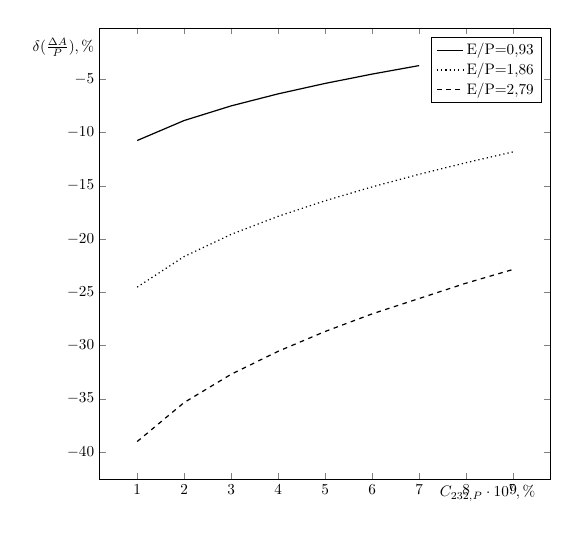
\begin{tikzpicture}[,
scale=0.55]
\begin{axis}[
  xlabel style = {{at={(axis description cs:.86,0)}}},
  ylabel = {$\delta(\frac{\Delta A}{P}), \%$},
  ylabel style = {{at={(axis description cs:-0.08,.925)},rotate=270,anchor=south}},
  xlabel = {$C_{232,P}\cdot10^{7}, \%$},
  width=12cm, height=12cm
]

\addplot+[mark=none,
  solid, black, thick
] coordinates {
  (1.0, -10.75592874548788)
  (2.0, -8.877549872366233)
  (3.0000000000000004, -7.50289958013979)
  (4.0, -6.3729908570898814)
  (5.0, -5.39405720345885)
  (6.0, -4.517136753769094)
  (7.000000000000001, -3.717964070419745)
};
\addlegendentry{{}{E/P=0,93}}

\addplot+[mark=none,
  dotted, black, thick
] coordinates {
  (1.0, -24.523693715258393)
  (2.0, -21.64946440952475)
  (3.0000000000000004, -19.56910789260241)
  (4.0, -17.87302824962024)
  (5.0, -16.41089275400384)
  (6.0, -15.109277255129713)
  (7.000000000000001, -13.927405951747463)
  (8.0, -12.837656298351746)
  (9.000000000000002, -11.820833744285492)
};
\addlegendentry{{}{E/P=1,86}}

\addplot+[mark=none,
  dashed, black, thick
] coordinates {
  (1.0, -39.02572435708815)
  (2.0, -35.35744140949972)
  (3.0000000000000004, -32.707361682832236)
  (4.0, -30.547279725027575)
  (5.0, -28.687040100935018)
  (6.0, -27.03315569727767)
  (8.0, -24.149000859531828)
  (9.000000000000002, -22.860928202940787)
};
\addlegendentry{{}{E/P=2,79}}

\end{axis}
\end{tikzpicture}


\caption{{Зависимость экономии работы разделения от ПДК $^{232}$U в НОУ-продукте с обогащением до уровня 4,95\% для различных $\frac{E}{P}$.{\label{sw495}}}}
    \end{minipage}%
    \begin{minipage}{.5\textwidth}
      \centering
      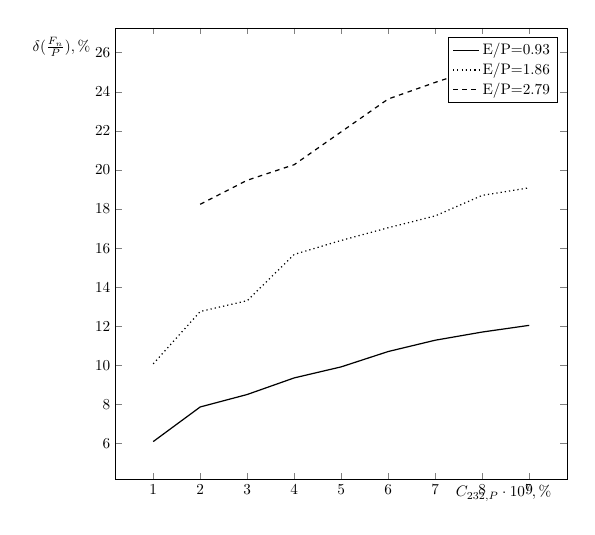
\begin{tikzpicture}[,
scale=0.55]
\begin{axis}[
  xlabel style = {{at={(axis description cs:.86,0)}}},
  ylabel = {$\delta(\frac{F_n}{P}), \%$},
  ylabel style = {{at={(axis description cs:-0.12,.925)},rotate=270,anchor=south}},
  xlabel = {$C_{232,P}\cdot10^{7}, \%$},
  width=12cm, height=12cm
]

\addplot+[mark=none,
  solid, black, thick
] coordinates {
  (1.0, 6.102609628967004)
  (2.0, 7.873257521230414)
  (3.0000000000000004, 8.510982187035465)
  (4.0, 9.359903696758797)
  (5.0, 9.924557345258734)
  (6.0, 10.709375471912841)
  (7.000000000000001, 11.287587970677283)
  (8.0, 11.705810902202751)
  (9.000000000000002, 12.048111265678951)
};
\addlegendentry{{}{E/P=0.93}}

\addplot+[mark=none,
  dotted, black, thick
] coordinates {
  (1.0, 10.07679447624098)
  (2.0, 12.756640615222503)
  (3.0000000000000004, 13.309773249935485)
  (4.0, 15.676539853992955)
  (5.0, 16.39235800951654)
  (6.0, 17.041722793102686)
  (7.000000000000001, 17.64593776461374)
  (8.0, 18.69753065296348)
  (9.000000000000002, 19.08456096001587)
};
\addlegendentry{{}{E/P=1.86}}

\addplot+[mark=none,
  dashed, black, thick
] coordinates {
  (2.0, 18.241079567317232)
  (3.0000000000000004, 19.47072745723193)
  (4.0, 20.268597025731783)
  (6.0, 23.628111214220738)
  (7.000000000000001, 24.476747414958155)
  (8.0, 25.273745846887998)
  (9.000000000000002, 25.337305198229632)
};
\addlegendentry{{}{E/P=2.79}}

\end{axis}
\end{tikzpicture}

    \caption{{Зависимость расхода природного урана от ПДК $^{232}$U в НОУ-продукте с обогащением до уровня 4,95\% для различных $\frac{E}{P}$.{\label{F0R495}}}}
\end{minipage}
\end{figure}


\begin{figure}[ht]
    \centering
    \begin{minipage}{.5\textwidth}
      \centering
      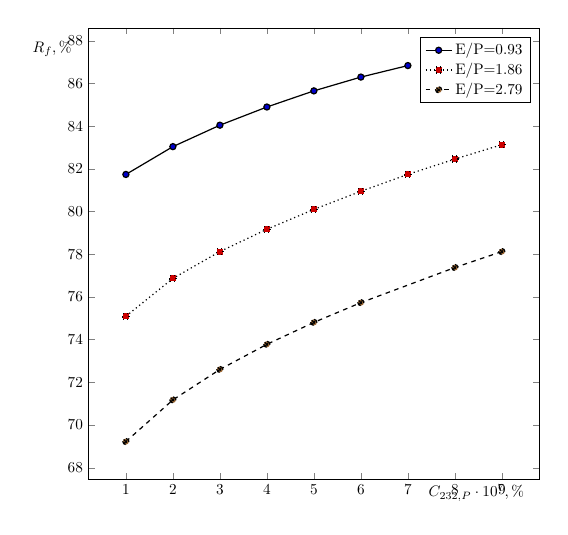
\begin{tikzpicture}[,
scale=0.55]
\begin{axis}[
  xlabel style = {{at={(axis description cs:.86,0)}}},
  ylabel = {$R_{f}, \%$},
  ylabel style = {{at={(axis description cs:-0.08,.925)},rotate=270,anchor=south}},
  xlabel = {$C_{232,P}\cdot10^{7}, \%$},
  width=12cm, height=12cm
]

\addplot+[
  solid, black, thick
] coordinates {
  (1.0, 81.73497884138504)
  (2.0, 83.03778477520555)
  (3.0000000000000004, 84.04194826713017)
  (4.0, 84.89394805905036)
  (5.0, 85.64964216184214)
  (6.0, 86.29627615264738)
  (7.000000000000001, 86.83475753524942)
};
\addlegendentry{{}{E/P=0.93}}

\addplot+[
  dotted, black, thick
] coordinates {
  (1.0, 75.09103641667504)
  (2.0, 76.86408581728926)
  (3.0000000000000004, 78.1230950450531)
  (4.0, 79.16703478387757)
  (5.0, 80.0973214088445)
  (6.0, 80.94802830843058)
  (7.000000000000001, 81.73831087619449)
  (8.0, 82.45610633767066)
  (9.000000000000002, 83.12799096181396)
};
\addlegendentry{{}{E/P=1.86}}

\addplot+[
  dashed, black, thick
] coordinates {
  (1.0, 69.22294832705394)
  (2.0, 71.17489372337026)
  (3.0000000000000004, 72.60072511995082)
  (4.0, 73.77803561909946)
  (5.0, 74.80542388393039)
  (6.0, 75.73053709257948)
  (8.0, 77.37433736075826)
  (9.000000000000002, 78.12192420776128)
};
\addlegendentry{{}{E/P=2.79}}

\end{axis}
\end{tikzpicture}


      \caption{{Зависимость степени извлечения $^{235}$U от ПДК $^{232}$U в НОУ-продукте с обогащением до уровня 4,95\% для различных $\frac{E}{P}$.{\label{ex495}}}}
    \end{minipage}%
    \begin{minipage}{.5\textwidth}
      \centering
      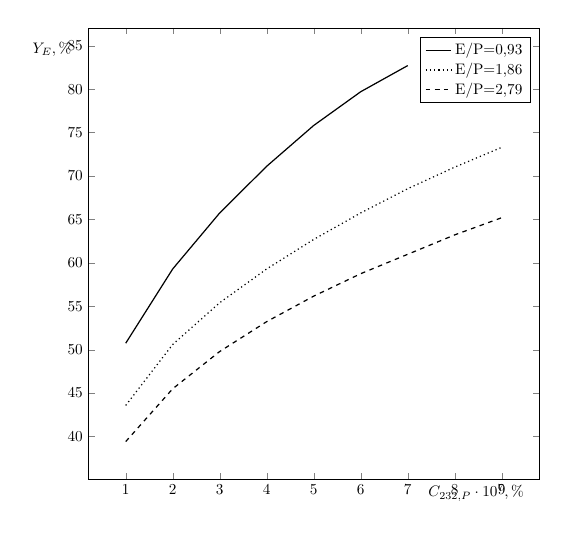
\begin{tikzpicture}[,
scale=0.55]
\begin{axis}[
  xlabel style = {{at={(axis description cs:.86,0)}}},
  ylabel = {$Y_{E}, \%$},
  ylabel style = {{at={(axis description cs:-0.08,.925)},rotate=270,anchor=south}},
  xlabel = {$C_{232,P}\cdot10^{7}, \%$},
  width=12cm, height=12cm
]

\addplot+[mark=none,
  solid, black, thick
] coordinates {
  (1.0, 50.745320366220234)
  (2.0, 59.30149726322195)
  (3.0000000000000004, 65.7519664106782)
  (4.0, 71.12954522207238)
  (5.0, 75.82763880377078)
  (6.0, 79.7135693705535)
  (7.000000000000001, 82.72543981227668)
};
\addlegendentry{{}{E/P=0,93}}

\addplot+[mark=none,
  dotted, black, thick
] coordinates {
  (1.0, 43.577905794327634)
  (2.0, 50.60187689534774)
  (3.0000000000000004, 55.41327633341921)
  (4.0, 59.30149726322195)
  (5.0, 62.69903149138577)
  (6.0, 65.75196641067834)
  (7.000000000000001, 68.5430309981216)
  (8.0, 71.02486897820552)
  (9.000000000000002, 73.30720710112764)
};
\addlegendentry{{}{E/P=1,86}}

\addplot+[mark=none,
  dashed, black, thick
] coordinates {
  (1.0, 39.414574744906304)
  (2.0, 45.501187547358626)
  (3.0000000000000004, 49.79017656124783)
  (4.0, 53.23340118139871)
  (5.0, 56.16715278135177)
  (6.0, 58.753339802423696)
  (8.0, 63.222220423599175)
  (9.000000000000002, 65.20220176963932)
};
\addlegendentry{{}{E/P=2,79}}

\end{axis}
\end{tikzpicture}


      \caption{{Зависимость степени извлечения $^{235}$U из регенерата от ПДК $^{232}$U в НОУ-продукте с обогащением до уровня 4,95\% для различных $\frac{E}{P}$.{\label{exR495}}}}
\end{minipage}
\end{figure}


    
На рисунках \ref{sw495}-\ref{F0R495} представлены зависимости от величины концентрации $^{232}$U, предельно допустимой в продукте, следующих интегральных параметров каскадной схемы: $\delta(\frac{\Delta A}{P})$ -- экономии работы разделения по сравнению с референтной схемы трехпоточного каскада для обогащения природного урана.(отрицательная величина означает перерасход работы разделения); степени извлечения $^{235}$U в схеме $Y_f$ и из регенерата $Y_{E}$, а также удельный расход природного урана $\frac{F_{NU}}{P}$. На каждом из рисунков представлено по три кривых, каждая их которых отвечает одному из рассмотренных значений параметра ($E/P$).

Анализ зависимостей, представленных на рис. \ref{sw44}-\ref{F0R495} позволяет сделать заключение о применимости схемы двойного каскада с НОУ-разбавителем для задачи полного возврата массы регенерата в ядерный топливный цикл в условиях многократного рецикла при одной и более единиц облученного топлива для производства одной единицы НОУ-продукта как в условиях более <<жестких>> (меньше $2\cdot10^{-7}$\%) ограничений на содержание $^{232}$U, чем современные требования, так и при увеличении допустимого порога концентрации $^{232}$U в НОУ-продукте. 
Таким же образом схема показывает свою устойчивость для различных требуемых $^{235}$U эффективных значениях концентрации в продукте. Отметим, что решения задачи были найдены во всех случаях, кроме нескольких точках на кривой для случая ($E/P=0,93$), где не удалось найти решений при увеличении допустимой концентрации $^{232}U$ в товарном НОУ. Такой результат связан с тем, что в случае ($E/P=0,93$) входящая в каскадную схема масса $^{232}$U является наименьшей и даже, несмотря на относительную загрязнённость регенерата данным изотопом, его исходной массы недостаточно, чтобы получить концентрацию этого изотопа на  уровне допустимого предела в товарном НОУ. Проще говоря, при $E/P=0,93$ невозможно найти решения, при которых концентрация $^{232}$U в товарном НОУ будет строго равна заданной предельной величине, а возможно только найти решения, для которых эта концентрация будет ниже. Естественно, получение концентрации $^{232}$U в продукте ниже допустимых пределов также можно рассматривать в качестве успешного решения поставленной задачи.  

Важно заметить, что снижение ограничений, которое может последовать за возможным изменением технологии процесса изготовления ТВЭЛов в будущем, позволит улучшить ключевые характеристики схемы.

В завершении еще раз подчеркнем, что исходя из анализа результатов, представленных на графиках \ref{sw44}-\ref{F0R495}, уменьшение допустимой концентрации $^{232}$U в продукте при фиксированном отношении исходного регенерата к товарному НОУ обусловливает ухудшение всех исследуемых ключевых показателей. Однако, из этих показателей, наиболее существенно падение степени извлечения $^{235}$U из регенерата при более строго ограничении на $^{232}$U, тогда как значительного увеличения расхода природного урана, увеличения числа центрифуг в каскадной схем (работы разделения), или значимого ухудшения извлечения $^{235}$U в схеме не наблюдается. И, самое главное, каскадная схема позволяет решить поставленную задачу для всех случаев.


\section{Общие выводы по результатам анализа схемы двойного каскада с НОУ-разбавителем}

В качестве обобщающих выводов по результатам анализа предложенной схемы двойного каскада с НОУ-разбавителем (рис. \ref{p2left}), обозначим следующее:
\begin{enumerate}
    \item схема применима для обогащения регенерированного урана в условиях многократного рецикла урана в топливе легководных реакторов, поскольку позволяет получать продукт, отвечающий всем требованиям на концентрации четных изотопов для регенерата различного исходного состава, включая рециклы, к которым накопилось повышенное содержание четных изотопов (на примере состава №2);
    \item схема показывает свою устойчивость в условиях изменения внешних ограничений и требований к получаемому продукту;
    \item схема позволяет отделить участки обогащения регенерированного урана (где разделительное оборудование будет подвержено загрязнению минорными изотопами) от каскадов, обогащающих не содержащий $^{232,236}$U природный уран или ОГФУ. При этом доля разделительных мощностей, отводимых под работу с регенерированным ураном при наработке НОУ для загрузки реактора составляет не более 10\%;
     \item в схеме происходит накопление побочно производимого материала -- высокоактивного отхода (отбор второго каскада), в котором к тому же происходит потеря делящегося $^{235}$U. Стратегии дальнейшего обращения с данным отходом требуют отдельного анализа, который будет проведен далее в Главе 4.
    \item работа схемы связана с потерями работы разделения при двух этапах производственного процесса:
    \begin{enumerate}
        \item обеднение отбора первого каскада $P_1$ во втором каскаде;
        \item смешивание потоков $W_2$ с НОУ-разбавителем $P_0$, в которых различается содержание изотопа $^{235}$U;
    \end{enumerate}
\end{enumerate}






\section{Рассмотрение различных возможностей утилизации легкой фракции второго каскада в схеме}

\subsection{Анализ возможности утилизации легкой фракции путем ее перемешивания с регенератом, поступающим на обогащение}

\subsubsection{Описание схемы двойного каскада с НОУ-разбавителем с возвратом потока $P_2$ в цикл}

В качестве модификации схемы двойного каскада с НОУ-разбавителем (рис. \ref{P2utilizationRing}), рассмотренной в предыдущем разделе, предложен способ, позволяющий вернуть поток $P_2$ в топливный цикл для производства НОУ-продукта (рис. \ref{p2left}) \cite{nevinicaToplivnyyCiklLegkovodnogo2019, nevinicaSposobIzotopnogoVosstanovleniya2019}. Принцип ее работы состоит в следующем.

\begin{figure}[ht]
    \centerfloat{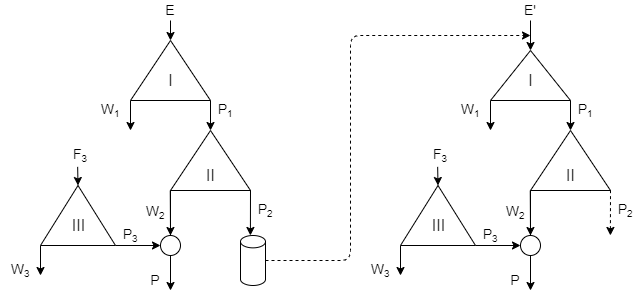
\includegraphics[scale=0.55]{cascades/P2utilizationRing}}
    \caption{Схема передачи загрязненной изотопом $^{232}$U фракции гексафторида урана в двойном каскаде от первой партии дообогащенного регенерированного урана к последующей. Обозначения: $E$ -- поток регенерированного урана; $P_1$ -- поток отбора первого каскада, выступающий питанием второго каскада; $W_1$ -- поток отвала первого каскада; $W_2$ -- поток тяжелой фракции (условный «отвал») второго каскада; $P_0$ -- поток НОУ-разбавителя; $P$ -- финальный продукт (товарный низкообогащенный уран (НОУ); $P_2$ -- поток отбора второго каскада, который подается на питание последующего двойного каскада, перемешиваясь с регенератом очередного рецикла}\label{P2utilizationRing}
\end{figure}

Учитывая, что каскадная схема двойного каскада с НОУ-разбавителем (рис. \ref{p2left}) предназначена для обогащения регенерата с высоким накопившимся в ходе серии пройденных рециклов содержанием изотопа $^{232}$U, можно использовать такую каскадную схему для вовлечения ранее полученного в потоке отбора второго каскада фракции $P_2$ загрязненной изотопом $^{232}$U. Выведенный ранее из системы гексафторида урана может быть перемешан с регенератом, полученным из следующей партии отработавшего топлива, то есть с составом более загрязненным изотопами $^{232,233,234,236}$U, чем исходно использовавшийся состав, побочным продуктом которого оказался этот $P_2$. Полученная таким образом в результате смешения $P_2$ предыдущего рецикла и регенерата очередного рецикла смесь будет отправлена на последующее обогащение (рис. \ref{P2utilizationRing}).

Исходя из идеи такой схемы, при ее использовании удастся полностью замкнуть топливный цикл по урану, а единственным отходом производства останется ОГФУ, образующийся в отвале первого каскада, который можно считать штатным отходом обогатительного производства с отработанными технологиями хранения и переработки. При этом после завершения производственного цикла останется невостребованным только та масса обогащенного по изотопу $^{232}$U гексафторида урана (загрязненной фракции легкого конца второго каскада (рис. \ref{P2utilizationRing})), которая будет образована после обогащения последней партии регенерата. Таким образом, предложенный подход к дообогащению регенерата урана позволяет организовать полный возврат массы регенерированного урана в топливный цикл в течение всего жизненного цикла задействованного урана.

При этом, такая схема, при схожем наборе достоинств и недостатков схемы двойного каскада с НОУ-разбавителем с возвратом потока $P_2$ в цикл (рис. \ref{P2utilizationRing}), в качестве достоинства схемы с возвратом $P_2$ предполагается более глубокая выработка потенциала делящегося $^{235}$U, накапливаемого совместно с изотопами $^{232,233,234}$U в загрязненной фракции второго каскада. Это должно позволить добиться меньших потерь $^{235}$U на всем жизненном цикле используемого урана.


Ранее, в работе \cite{nevinicaToplivnyyCiklLegkovodnogo2019}, было показано, что предложенная схема рециклирования действительно позволяет полностью израсходовать и исходный регенерированный уран и образующийся в результате использования двойного каскада высокообогащенный отход, реализовав вышеупомянутые достоинства схемы. Следующим шагом должна стать оценка интегральных показателей для рассматриваемой схемы в условиях ее использования для обогащения регенерированного урана и наработки НОУ для обеспечения поставок для формирования топлива нескольких последовательных загрузок реактора.

Для этого рассмотрим постановку задачи возврата регенерированного урана с последующим замыканием $P_2$, на основе описанной в разделе \ref{triple_descr} каскадной схемы. В качестве разделяемой смеси выбран регенерированный уран, испытавший несколько циклов облучения, а именно состав 2 в таблица \ref{is_compositions_2_5} \cite{smirnovObogashchenieRegenerirovannogoUrana2018}. Требуемая концентрация $^{235}$U в конечном продукте задана равной 4,95\%, коэффициент компенсации реактивности 0,29. Величину коэффициента разделения на единичную разность массовых чисел выбрали равной 1,2. Концентрации $^{235}$U в потоках отвала каскада 1 и каскада для наработки разбавителя задали равной 0,1\%. Ограничение по концентрации $^{232}$U соответствовало $5\cdot10^{-7} \%$, а отношение масс <<исходный регенерат/товарный НОУ>> выбрано равным 0,93 \cite{smirnovObogashchenieRegenerirovannogoUrana2018}.  При решении задачи оптимизации с переменными значениями концентраций $^{235}$U в потоках отборов $P_1$ и $P_2$, описанном выше, значения величин массовых чисел опорных компонент ($M_{k1}$ и $M_{k2}$) был выбран исходя из найденных ранее оптимальных решений. Алгоритм для расчета каскадной схемы описан в \ref{statement}

Последовательность перегрузок можно описать следующим образом. Из рассматриваемого исходного состава регенерата изготавливают сначала топливо для первой перегрузки. Далее, загрязненную фракцию от обогащения регенерата для первой перегрузки перемешивают с регенератом исходного состава для второго рецикла и направляют на последующее обогащение для получения топлива следующей перегрузки. В итоге рассматривается 7 перегрузок. При расчете состава низкообогащенного урана после каскада при получении топлива для каждой из перегрузок решается оптимизационную задачу, алгоритм которой описан в \ref{statement}.

Заметим, что процесс возврата данного материала в воспроизводство низкообогащенного урана может быть начат также и после дообогащения регенерата уже для одной ТВС и даже для ее части (непрерывный возврат). В этом случае также удастся полностью замкнуть топливный цикл по урану, а единственным отходом производства станет обедненный гексафторид, образующийся в отвале первого каскада, который можно считать штатным отходом обогатительного производства, для которого на сегодняшний день отработаны технологии хранения и переработки.

При этом после вывода завода из эксплуатации (или остановки на планово-предупредительный ремонт) останется невостребованным только та масса обогащенного по изотопу $^{232}$U гексафторида урана, которая будет образована после обогащения последней партии регенерата на этом заводе. Таким образом, рассматриваемый подход к дообогащению регенерата урана позволяет организовать полный возврат регенерированного урана в топливный цикл в течение практически всего жизненного цикла топлива легководных реакторов, работающих в замкнутом топливном цикле. Однако,несмотря на очевидные достоинства рассматриваемого способа, возникает вопрос о его эффективности с точки зрения интегральных характеристик разделительного каскада, важных для экономики топливного цикла в целом. Речь идет об экономии природного урана в цикле и затратах работы разделения на единицу массы готового НОУ.


Ввиду сложности многокритериального анализа для каждой из перегрузок был рассмотрен случай с параллельными «ветками», на каждой из которых проводили последовательный расчет изотопных составов и параметров разделительного каскада для семи перегрузок, при условии оптимизации на каждом из шагов по одному и тому же критерию эффективности. В качестве критериев эффективности выступали величины: (1) минимум расхода природного урана на единицу продукта, (2) минимум затрат работы разделения на единицу продукта, (3) минимум массы отхода двойного каскада, (4) минимум концентрации изотопа $^{232}$U (в диапазоне 2-$5\cdot10^{-7}$\%), (5) минимум концентрации изотопа $^{236}$U, (6) максимум степени извлечения $^{235}$U из поступающего в обогащение регенерата (\ref{RecR2}). Смысл критериев (1), (2) и (6) описан в \ref{criteria_list}. Представленные номера критериев соответствуют обозначениям кривых для рис. \ref{7}–\ref{13}. Под степенью извлечения $^{235}$U из исходного регенерированного урана понимали отношение массы $^{235}$U в отвале второго каскада к массе $^{235}$U в исходной смеси регенерата, поступившего для обогащения. В числе прочих обозначений, используются потоки: $E$ – поток питающего каскадную схему регенерата, $P$ -- товарный НОУ.


Далее представлены результаты проведенных вычислительных экспериментов и проведен их анализ.

На рисунке \ref{3} представлено изменение удельного расхода природного урана при получении товарного НОУ при шести различных критериях эффективности, по которым осуществляли оптимизацию для каждой перегрузки. Как следует из анализа зависимостей (рис. \ref{3}-\ref{6})), показанных на указанном рисунке при оптимизации по четырем, а именно: минимуму удельного расхода природного урана, минимуму удельных затрат работы разделения, минимуму массы отхода двойного каскада, максимуму степени извлечения $^{235}$U из поступающего в обогащение регенерата, зависимости практически совпадают. Это можно объяснить тем, что данные критерии близки по своей сути. Например, максимум степени извлечения $^{235}$U из поступающего в обогащение регенерата должен приводить к необходимости использования минимальной массы $^{235}$U из природного сырья, что и выражается в уменьшении расхода природного сырья. В целом все кривые представляют собой уменьшающиеся функции, что логично, учитывая, что с каждой перегрузкой масса исходного регенерата возрастает одновременно с повышением концентрации $^{235}$U в нем.


\begin{figure}[ht]
    \centering
    \begin{minipage}{.5\textwidth}
      \centering
      \begin{tikzpicture}[,
scale=0.95]
\begin{axis}[
  xlabel style = {{at={(axis description cs:.86,0)}}},
  ylabel = {$\delta(\frac{F_{NU}}{P}), \%$},
  ylabel style = {{at={(axis description cs:-0.08,.94)},rotate=270,anchor=south}},
  xlabel = {$i$},
  width=16cm, height=16cm, xtick={1,2,3,4,5,6,7}
]

\addplot+[
  solid, green, thin
] coordinates {
  (1.0, 9.60224940765123)
  (2.0, 10.471964607421514)
  (3.0, 10.328677265019726)
  (4.0, 10.937722799772365)
  (5.0, 11.551073258460454)
  (6.0, 11.482634526238378)
  (7.0, 11.495414262020132)
};
\addlegendentry{{}{$(Y_f)_\text{max}$}}

\addplot+[
  dotted, red, thick
] coordinates {
  (1.0, 9.60224940765123)
  (2.0, 10.471964607421514)
  (3.0, 10.328677265019726)
  (4.0, 10.937722799772365)
  (5.0, 11.551073258460454)
  (6.0, 11.482634526238378)
  (7.0, 11.495414262020132)
};
\addlegendentry{{}{$(Y_{E})_\text{max}$}}

\addplot+[
  dashed, black, thick
] coordinates {
  (1.0, 9.758344663807906)
  (2.0, 10.377586059230682)
  (3.0, 10.148945832377942)
  (4.0, 11.036603656094378)
  (5.0, 11.596700175896046)
  (6.0, 11.502422364899322)
  (7.0, 11.5042389394856)
};
\addlegendentry{{}{$(\delta(\frac{\Delta A}{P}))_\text{min}$}}

\addplot+[
  dashdotted, brown, thick
] coordinates {
  (1.0, 10.428757919569875)
  (2.0, 11.091940883100326)
  (3.0, 11.132231272182302)
  (4.0, 11.940825541138867)
  (5.0, 12.240045586112991)
  (6.0, 12.233596137265634)
  (7.0, 12.281186997924387)
};
\addlegendentry{{}{$(\delta(\frac{F_{NU}}{P}))_\text{min}$}}

\addplot+[
  solid, teal, thin
] coordinates {
  (1.0, 9.758344663807906)
  (2.0, 10.377586059230682)
  (3.0, 10.148945832377942)
  (4.0, 11.415331124937522)
  (5.0, 11.403205816515582)
  (6.0, 11.411528711119201)
  (7.0, 11.462271406331004)
};
\addlegendentry{{}{$(\frac{P_2}{P})_\text{min}$}}

\end{axis}
\end{tikzpicture}


      \caption{{Зависимость удельного расхода природного урана в двойном каскаде с замыканием в зависимости от номера перегрузки для обогащения 4,95\% для различных критериев эффективности.{\label{3}}}}
    \end{minipage}%
    \begin{minipage}{.5\textwidth}
      \centering
      \begin{tikzpicture}[,
scale=0.95,
scale=0.95]
\begin{axis}[
  xlabel style = {{at={(axis description cs:.86,0)}}},
  ylabel = {$R_{RepU}, \%$},
  ylabel style = {{at={(axis description cs:-0.08,.925)},rotate=270,anchor=south}},
  xlabel = {$i$},
  width=16cm, height=16cm
]

\addplot+[
  solid, black, thick
] coordinates {
  (1.0, 72.8241808435042)
  (2.0, 66.68566594907492)
  (3.0, 58.35228156487533)
  (4.0, 56.643420943442365)
  (5.0, 56.21679099162951)
  (6.0, 54.184876916297)
  (7.0, 52.553320781875414)
};
\addlegendentry{{}{$(R_f)_\text{max}$}}

\addplot+[
  dotted, black, thick
] coordinates {
  (1.0, 72.8241808435042)
  (2.0, 66.68566594907492)
  (3.0, 58.35228156487533)
  (4.0, 56.643420943442365)
  (5.0, 56.21679099162951)
  (6.0, 54.184876916297)
  (7.0, 52.553320781875414)
};
\addlegendentry{{}{$(R_{RepU})_\text{max}$}}

\addplot+[
  dashed, black, thick
] coordinates {
  (1.0, 73.82998902426432)
  (2.0, 66.64446941870102)
  (3.0, 57.19448148394325)
  (4.0, 56.67546946948041)
  (5.0, 56.226760998555434)
  (6.0, 54.188337945615274)
  (7.0, 52.5546392882073)
};
\addlegendentry{{}{$(\delta(\frac{\Delta U}{P}))_\text{min}$}}

\addplot+[
  dashdotted, black, thick
] coordinates {
  (1.0, 73.75583473104476)
  (2.0, 66.44811675745768)
  (3.0, 58.2996545335423)
  (4.0, 57.50685876177931)
  (5.0, 55.96223087076096)
  (6.0, 53.951506368752476)
  (7.0, 52.3277838935582)
};
\addlegendentry{{}{$(\delta(\frac{F_{NU}}{P}))_\text{min}$}}

\addplot+[
  solid, red, thick
] coordinates {
};
\addlegendentry{{}{$(C_{232,P})_\text{min}$}}

\addplot+[
  solid, blue, thick
] coordinates {
};
\addlegendentry{{}{$(C_{236,P})_\text{min}$}}

\addplot+[
  solid, brown, thick
] coordinates {
  (1.0, 73.82998902426432)
  (2.0, 66.64446941870102)
  (3.0, 57.19448148394325)
  (4.0, 58.460758694419646)
  (5.0, 56.177556015313)
  (6.0, 54.169304400774244)
  (7.0, 52.547895768556174)
};
\addlegendentry{{}{$(\frac{P_2}{P})_\text{min}$}}

\end{axis}
\end{tikzpicture}


\caption{{Степень извлечения $^{235}$U из исходного регенерата в двойном каскаде с замыканием в зависимости от номера перегрузки для обогащения 4,95\% для различных критериев эффективности.{\label{4}}}}
\end{minipage}
\end{figure}



\begin{figure}[ht]
    \centering
    \begin{minipage}{.5\textwidth}
      \centering
      \begin{tikzpicture}[,
scale=0.95,
scale=0.95]
\begin{axis}[
  xlabel style = {{at={(axis description cs:.86,0)}}},
  ylabel = {$\delta(\frac{P_{2}}{P}), \%$},
  ylabel style = {{at={(axis description cs:-0.08,.94)},rotate=270,anchor=south}},
  xlabel = {$i$},
  width=16cm, height=16cm, xtick={1,2,3,4,5,6,7}
]

\addplot+[
  solid, green, thin
] coordinates {
  (1.0, 1.0810960189992584)
  (2.0, 1.6146633333341598)
  (3.0, 2.3687024775347747)
  (4.0, 3.159113715125525)
  (5.0, 3.0809753572386254)
  (6.0, 3.3558969337102944)
  (7.0, 3.621806533418627)
};
\addlegendentry{{}{$(Y_f)_\text{max}$}}

\addplot+[
  dotted, red, thick
] coordinates {
  (1.0, 1.0810960189992584)
  (2.0, 1.6146633333341598)
  (3.0, 2.3687024775347747)
  (4.0, 3.159113715125525)
  (5.0, 3.0809753572386254)
  (6.0, 3.3558969337102944)
  (7.0, 3.621806533418627)
};
\addlegendentry{{}{$(Y_{E})_\text{max}$}}

\addplot+[
  dashed, black, thick
] coordinates {
  (1.0, 0.9191318565385409)
  (2.0, 1.5995427357743446)
  (3.0, 2.4336632372639344)
  (4.0, 3.1886436788896333)
  (5.0, 3.0921075113377343)
  (6.0, 3.3608476613695917)
  (7.0, 3.6241033759848253)
};
\addlegendentry{{}{$(\delta(\frac{\Delta A}{P}))_\text{min}$}}

\addplot+[
  dashdotted, brown, thick
] coordinates {
  (1.0, 0.9234810348382065)
  (2.0, 1.612721145807963)
  (3.0, 2.3724712118887568)
  (4.0, 2.9252605855990694)
  (5.0, 3.0737574380632946)
  (6.0, 3.3714004647467988)
  (7.0, 3.6482779696747203)
};
\addlegendentry{{}{$(\delta(\frac{F_{NU}}{P}))_\text{min}$}}

\addplot+[
  solid, teal, thin
] coordinates {
  (1.0, 0.9191318565385409)
  (2.0, 1.5995427357743446)
  (3.0, 2.4336632372639344)
  (4.0, 2.7304942598358695)
  (5.0, 3.036681544811821)
  (6.0, 3.3363360013335974)
  (7.0, 3.6127481585062196)
};
\addlegendentry{{}{$(\frac{P_2}{P})_\text{min}$}}

\end{axis}
\end{tikzpicture}


      \caption{{Зависимость величины удельного отхода (на единицу продукта) в зависимости от номера перегрузки для обогащения 4,95\% для различных критериев эффективности.{\label{5}}}}
    \end{minipage}%
    \begin{minipage}{.5\textwidth}
      \centering
      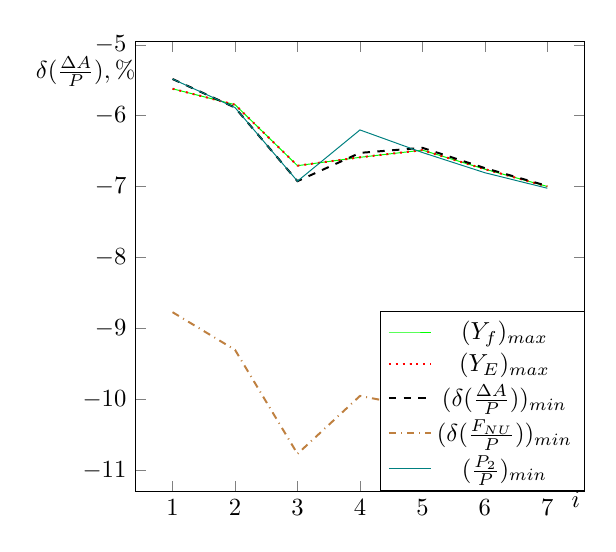
\begin{tikzpicture}[,
scale=0.89]
\begin{axis}[
  xlabel style = {{at={(axis description cs:.98,0.02)}}},
  ylabel = {$\delta(\frac{\Delta A}{P}), \%$},
  ylabel style = {{at={(axis description cs:-0.11,.88)},rotate=270,anchor=south}},
  xlabel = {$i$},
  width=8cm, height=8cm, xtick={1,2,3,4,5,6,7}, legend style={at={(1,0)},anchor=south east}
]

\addplot+[mark=none,
  solid, green, thin
] coordinates {
  (1.0, -5.619564224321039)
  (2.0, -5.84441657242741)
  (3.0, -6.704917867424845)
  (4.0, -6.586866390801599)
  (5.0, -6.485554729454776)
  (6.0, -6.754284481908828)
  (7.0, -6.998000929961407)
};
\addlegendentry{{}{$(Y_f)_\text{max}$}}

\addplot+[mark=none,
  dotted, red, thick
] coordinates {
  (1.0, -5.619564224321039)
  (2.0, -5.84441657242741)
  (3.0, -6.704917867424845)
  (4.0, -6.586866390801599)
  (5.0, -6.485554729454776)
  (6.0, -6.754284481908828)
  (7.0, -6.998000929961407)
};
\addlegendentry{{}{$(Y_{E})_\text{max}$}}

\addplot+[mark=none,
  dashed, black, thick
] coordinates {
  (1.0, -5.482150178426482)
  (2.0, -5.884813687357447)
  (3.0, -6.923308229121754)
  (4.0, -6.524186589001574)
  (5.0, -6.4527000666451135)
  (6.0, -6.739088245807983)
  (7.0, -6.991066392896656)
};
\addlegendentry{{}{$(\delta(\frac{\Delta A}{P}))_\text{min}$}}

\addplot+[mark=none,
  dashdotted, brown, thick
] coordinates {
  (1.0, -8.771994897379303)
  (2.0, -9.303209789751323)
  (3.0, -10.770438360555245)
  (4.0, -9.953392791027085)
  (5.0, -10.122163189828624)
  (6.0, -10.411774829351534)
  (7.0, -10.654096806225095)
};
\addlegendentry{{}{$(\delta(\frac{F_{NU}}{P}))_\text{min}$}}

\addplot+[mark=none,
  solid, teal, thin
] coordinates {
  (1.0, -5.482150178426482)
  (2.0, -5.884813687357447)
  (3.0, -6.923308229121754)
  (4.0, -6.2006153993959785)
  (5.0, -6.519171025702167)
  (6.0, -6.804418040883925)
  (7.0, -7.023084861927327)
};
\addlegendentry{{}{$(\frac{P_2}{P})_\text{min}$}}

\end{axis}
\end{tikzpicture}


\caption{{Зависимость экономии работы разделения в зависимости от номера перегрузки для обогащения 4,95\% для различных критериев оптимальности.{\label{6}}}}
\end{minipage}
\end{figure}

В результате описанных выше процессов увеличивается и достигает значений, близких к 2, величина отношения (исходный регенерат)/продукт (риc. \ref{7}). Анализ зависимостей концентраций $^{235}$U и четных изотопов в регенерате, поступающем на обогащение после смешивания с высокообогащенной фракцией показывает, что все они повышается с каждой перегрузкой (рисунки \ref{8}–\ref{11}). Однако при использовании в качестве критериев эффективности минимумов концентраций  $^{232}$U и  $^{236}$U в товарном НОУ концентрации всех указанных выше изотопов в исходном регенерате возрастают заметно интенсивнее. Важно при этом отметить, что на последних перегрузках концентрация $^{235}$U в исходном регенерате превышает величину, требуемую для финального продукта (рисунок \ref{11}). Это означает, что схема начинает обеднять смесь и «чистить» ее от четных, а не обогащать. Особенно сильно это проявляется при минимизации концентраций четных изотопов в продукте, поскольку в этих случаях концентрация $^{235}$U в исходном регенерате могут приближаться к 5\% (рисунок \ref{10}). Подобные результаты говорят, в первую очередь, о нецелесообразности использования схемы в таком варианте для последовательного обогащения регенерата нескольких перегрузок с использованием в качестве критериев эффективности на каждом шаге требования минимальности концентраций $^{232}$U и  $^{236}$U в товарном НОУ. Однако требуют дополнительных исследований возможности дальнейшей модификации предложенной схемы, в том числе, для более эффективного использования исходного регенерата с повышенным содержанием $^{235}$U. Одним из таких вариантов может стать расширение диапазона увеличения концентрации  $^{235}$U в схеме, например, до 90\%. Другие варианты могут быть основаны на введении дополнительных потоков для разбавления четных изотопов и снижения концентрации  $^{235}$U до нужных значений.


\begin{figure}[ht]
    \centering
    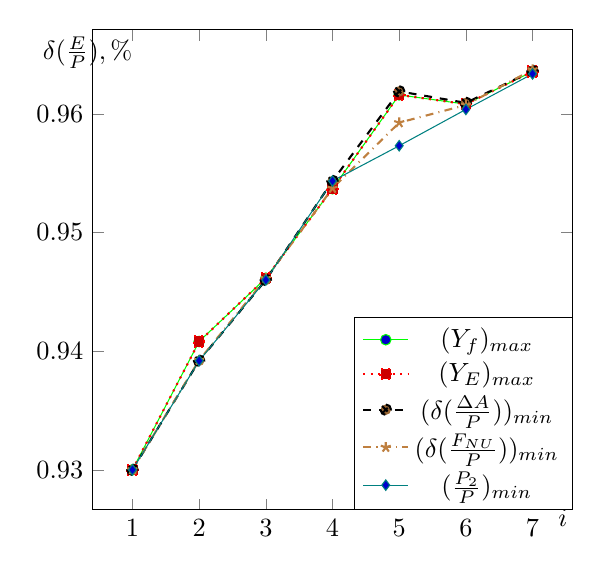
\begin{tikzpicture}[,
scale=0.95]
\begin{axis}[
  xlabel style = {{at={(axis description cs:.98,0.02)}}},
  ylabel = {$\delta(\frac{E}{P}), \%$},
  ylabel style = {{at={(axis description cs:-0.01,.9)},rotate=270,anchor=south}},
  xlabel = {$i$},
  width=8cm, height=8cm, xtick={1,2,3,4,5,6,7}, legend style={at={(1,0)},anchor=south east}
]

\addplot+[
  solid, green, thin
] coordinates {
  (1.0, 0.93)
  (2.0, 0.9408109601899927)
  (3.0, 0.9461466333333417)
  (4.0, 0.9536870247753478)
  (5.0, 0.9615911371512553)
  (6.0, 0.9608097535723863)
  (7.0, 0.9635589693371029)
};
\addlegendentry{{}{$(Y_f)_\text{max}$}}

\addplot+[
  dotted, red, thick
] coordinates {
  (1.0, 0.93)
  (2.0, 0.9408109601899927)
  (3.0, 0.9461466333333417)
  (4.0, 0.9536870247753478)
  (5.0, 0.9615911371512553)
  (6.0, 0.9608097535723863)
  (7.0, 0.9635589693371029)
};
\addlegendentry{{}{$(Y_{E})_\text{max}$}}

\addplot+[
  dashed, black, thick
] coordinates {
  (1.0, 0.93)
  (2.0, 0.9391913185653855)
  (3.0, 0.9459954273577434)
  (4.0, 0.9543366323726394)
  (5.0, 0.9618864367888964)
  (6.0, 0.9609210751133774)
  (7.0, 0.963608476613696)
};
\addlegendentry{{}{$(\delta(\frac{\Delta A}{P}))_\text{min}$}}

\addplot+[
  dashdotted, brown, thick
] coordinates {
  (1.0, 0.93)
  (2.0, 0.9392348103483821)
  (3.0, 0.9461272114580797)
  (4.0, 0.9537247121188877)
  (5.0, 0.9592526058559907)
  (6.0, 0.960737574380633)
  (7.0, 0.963714004647468)
};
\addlegendentry{{}{$(\delta(\frac{F_{NU}}{P}))_\text{min}$}}

\addplot+[
  solid, teal, thin
] coordinates {
  (1.0, 0.93)
  (2.0, 0.9391913185653855)
  (3.0, 0.9459954273577434)
  (4.0, 0.9543366323726394)
  (5.0, 0.9573049425983587)
  (6.0, 0.9603668154481183)
  (7.0, 0.963363360013336)
};
\addlegendentry{{}{$(\frac{P_2}{P})_\text{min}$}}

\end{axis}
\end{tikzpicture}


    \caption{Зависимость отношения потоков исходного регенерата и финального продукта (товарного НОУ) от номера перегрузки для обогащения 4,95\% для различных критериев эффективности.}\label{7}
\end{figure}



\begin{figure}[ht]
    \centering
    \begin{minipage}{.5\textwidth}
      \centering
      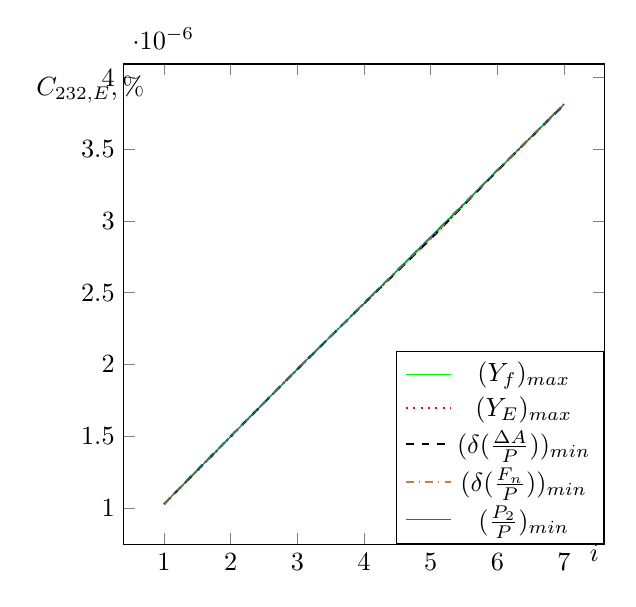
\begin{tikzpicture}[,
scale=0.95]
\begin{axis}[
  xlabel style = {{at={(axis description cs:.98,0.02)}}},
  ylabel = {$C_{232,E}, \%$},
  ylabel style = {{at={(axis description cs:-0.07,.9)},rotate=270,anchor=south}},
  xlabel = {$i$},
  width=8cm, height=8cm, xtick={1,2,3,4,5,6,7}, legend style={at={(1,0)},anchor=south east}
]

\addplot+[mark=none,
  solid, green, thin
] coordinates {
  (1.0, 1.0258e-6)
  (2.0, 1.4957859253750262e-6)
  (3.0, 1.9664961607465805e-6)
  (4.0, 2.4263137653178574e-6)
  (5.0, 2.8778904991462944e-6)
  (6.0, 3.3521276901753137e-6)
  (7.0, 3.8130792268330165e-6)
};
\addlegendentry{{}{$(Y_f)_\text{max}$}}

\addplot+[mark=none,
  dotted, red, thick
] coordinates {
  (1.0, 1.0258e-6)
  (2.0, 1.4957859253750262e-6)
  (3.0, 1.9664961607465805e-6)
  (4.0, 2.4263137653178574e-6)
  (5.0, 2.8778904991462944e-6)
  (6.0, 3.3521276901753137e-6)
  (7.0, 3.8130792268330165e-6)
};
\addlegendentry{{}{$(Y_{E})_\text{max}$}}

\addplot+[mark=none,
  dashed, black, thick
] coordinates {
  (1.0, 1.0258e-6)
  (2.0, 1.4983651087539599e-6)
  (3.0, 1.966794869704306e-6)
  (4.0, 2.424641617685412e-6)
  (5.0, 2.8770017284534706e-6)
  (6.0, 3.351739961430355e-6)
  (7.0, 3.812886476915959e-6)
};
\addlegendentry{{}{$(\delta(\frac{\Delta A}{P}))_\text{min}$}}

\addplot+[mark=none,
  dashdotted, brown, thick
] coordinates {
  (1.0, 1.0258e-6)
  (2.0, 1.4990615983803834e-6)
  (3.0, 1.967973359837115e-6)
  (4.0, 2.428311055154392e-6)
  (5.0, 2.8875886094436138e-6)
  (6.0, 3.355665432112993e-6)
  (7.0, 3.816382169516411e-6)
};
\addlegendentry{{}{$(\delta(\frac{F_n}{P}))_\text{min}$}}

\addplot+[mark=none,
  solid, teal, thin
] coordinates {
  (1.0, 1.0258e-6)
  (2.0, 1.4983651087539599e-6)
  (3.0, 1.966794869704306e-6)
  (4.0, 2.424641617685412e-6)
  (5.0, 2.8907700275574118e-6)
  (6.0, 3.3536492768045208e-6)
  (7.0, 3.8138187754759447e-6)
};
\addlegendentry{{}{$(\frac{P_2}{P})_\text{min}$}}

\end{axis}
\end{tikzpicture}


      \caption{{Зависимость концентрации $^{232}$U в исходном регенерате от номера перегрузки для обогащения 4,95\% для различных критериев эффективности.{\label{8}}}}
    \end{minipage}%
    \begin{minipage}{.5\textwidth}
      \centering
      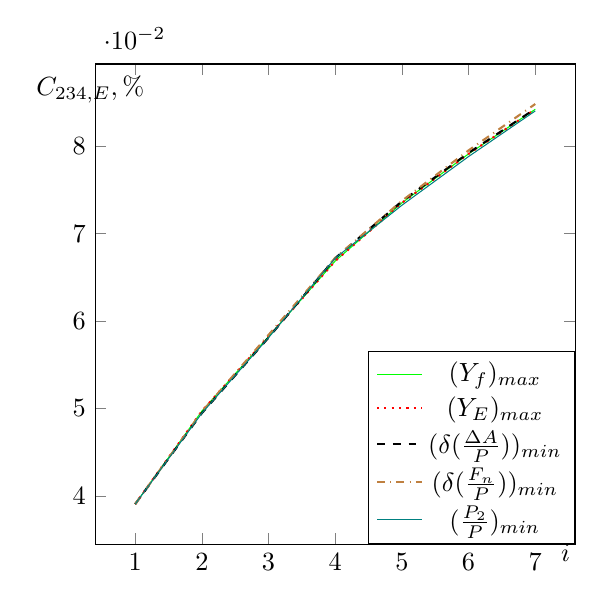
\begin{tikzpicture}[,
scale=0.95]
\begin{axis}[
  xlabel style = {{at={(axis description cs:.98,0.02)}}},
  ylabel = {$C_{234,E}, \%$},
  ylabel style = {{at={(axis description cs:-0.01,.9)},rotate=270,anchor=south}},
  xlabel = {$i$},
  width=8cm, height=8cm, xtick={1,2,3,4,5,6,7}, legend style={at={(1,0)},anchor=south east}
]

\addplot+[mark=none,
  solid, green, thin
] coordinates {
  (1.0, 0.039067000000000005)
  (2.0, 0.04970009905714201)
  (3.0, 0.05822673196432028)
  (4.0, 0.066871941585519)
  (5.0, 0.07352173483973685)
  (6.0, 0.07912564215270304)
  (7.0, 0.0842247287548398)
};
\addlegendentry{{}{$(Y_f)_\text{max}$}}

\addplot+[mark=none,
  dotted, red, thick
] coordinates {
  (1.0, 0.039067000000000005)
  (2.0, 0.04970009905714201)
  (3.0, 0.05822673196432028)
  (4.0, 0.066871941585519)
  (5.0, 0.07352173483973685)
  (6.0, 0.07912564215270304)
  (7.0, 0.0842247287548398)
};
\addlegendentry{{}{$(Y_{E})_\text{max}$}}

\addplot+[mark=none,
  dashed, black, thick
] coordinates {
  (1.0, 0.039067000000000005)
  (2.0, 0.04946841865210639)
  (3.0, 0.05810622920978174)
  (4.0, 0.06719588044561586)
  (5.0, 0.07370160217404174)
  (6.0, 0.07923292102134907)
  (7.0, 0.08429019401800651)
};
\addlegendentry{{}{$(\delta(\frac{\Delta A}{P}))_\text{min}$}}

\addplot+[mark=none,
  dashdotted, brown, thick
] coordinates {
  (1.0, 0.039067000000000005)
  (2.0, 0.049622790256222765)
  (3.0, 0.05841925622359249)
  (4.0, 0.06723365201075267)
  (5.0, 0.07375289742007517)
  (6.0, 0.07952538996328075)
  (7.0, 0.0848299502052639)
};
\addlegendentry{{}{$(\delta(\frac{F_n}{P}))_\text{min}$}}

\addplot+[mark=none,
  solid, teal, thin
] coordinates {
  (1.0, 0.039067000000000005)
  (2.0, 0.04946841865210639)
  (3.0, 0.05810622920978174)
  (4.0, 0.06719588044561586)
  (5.0, 0.0732483046560336)
  (6.0, 0.07882038255016108)
  (7.0, 0.08403644927222485)
};
\addlegendentry{{}{$(\frac{P_2}{P})_\text{min}$}}

\end{axis}
\end{tikzpicture}


\caption{{Зависимость концентрации $^{234}$U в исходном регенерате от номера перегрузки для обогащения 4,95\% для различных критериев эффективности.{\label{9}}}}
\end{minipage}
\end{figure}


\begin{figure}[ht]
    \centering
    \begin{minipage}{.5\textwidth}
      \centering
      \begin{tikzpicture}[,
scale=0.95,
scale=0.95,
scale=0.95,
scale=0.95]
\begin{axis}[
  xlabel style = {{at={(axis description cs:.86,0)}}},
  ylabel = {$C_{235,E}, \%$},
  ylabel style = {{at={(axis description cs:-0.05,.94)},rotate=270,anchor=south}},
  xlabel = {$i$},
  width=16cm, height=16cm, xtick={1,2,3,4,5,6,7}
]

\addplot+[
  solid, green, thin
] coordinates {
  (1.0, 1.0675000000000001)
  (2.0, 1.25936050072558)
  (3.0, 1.3865672666089406)
  (4.0, 1.5318691629561354)
  (5.0, 1.6160275951289529)
  (6.0, 1.6670280878275427)
  (7.0, 1.7186620013589922)
};
\addlegendentry{{}{$(Y_f)_\text{max}$}}

\addplot+[
  dotted, red, thick
] coordinates {
  (1.0, 1.0675000000000001)
  (2.0, 1.25936050072558)
  (3.0, 1.3865672666089406)
  (4.0, 1.5318691629561354)
  (5.0, 1.6160275951289529)
  (6.0, 1.6670280878275427)
  (7.0, 1.7186620013589922)
};
\addlegendentry{{}{$(Y_{E})_\text{max}$}}

\addplot+[
  dashed, black, thick
] coordinates {
  (1.0, 1.0675000000000001)
  (2.0, 1.2504710937036378)
  (3.0, 1.3836298662534239)
  (4.0, 1.5442795434551526)
  (5.0, 1.6209850102079988)
  (6.0, 1.669124592110755)
  (7.0, 1.7195891125167035)
};
\addlegendentry{{}{$(\delta(\frac{\Delta A}{P}))_\text{min}$}}

\addplot+[
  dashdotted, brown, thick
] coordinates {
  (1.0, 1.0675000000000001)
  (2.0, 1.251328369665262)
  (3.0, 1.3861900168691095)
  (4.0, 1.5325896194737838)
  (5.0, 1.6071563406244789)
  (6.0, 1.6656685168444958)
  (7.0, 1.7215649931745327)
};
\addlegendentry{{}{$(\delta(\frac{F_{NU}}{P}))_\text{min}$}}

\addplot+[
  solid, teal, thin
] coordinates {
  (1.0, 1.0675000000000001)
  (2.0, 1.2504710937036378)
  (3.0, 1.3836298662534239)
  (4.0, 1.5442795434551526)
  (5.0, 1.6007731300663814)
  (6.0, 1.6586814764166735)
  (7.0, 1.714997939379093)
};
\addlegendentry{{}{$(\frac{P_2}{P})_\text{min}$}}

\end{axis}
\end{tikzpicture}


      \caption{{Зависимость концентрации $^{235}$U в исходном регенерате от номера перегрузки для обогащения 4,95\% для различных критериев эффективности.{\label{10}}}}
    \end{minipage}%
    \begin{minipage}{.5\textwidth}
      \centering
      \begin{tikzpicture}[,
scale=0.95,
scale=0.95,
scale=0.95,
scale=0.95]
\begin{axis}[
  xlabel style = {{at={(axis description cs:.86,0)}}},
  ylabel = {$C_{236,E}, \%$},
  ylabel style = {{at={(axis description cs:-0.05,.94)},rotate=270,anchor=south}},
  xlabel = {$i$},
  width=16cm, height=16cm, xtick={1,2,3,4,5,6,7}
]

\addplot+[
  solid, green, thin
] coordinates {
  (1.0, 1.4458)
  (2.0, 1.5766817339001622)
  (3.0, 1.6449480750353955)
  (4.0, 1.740165734281792)
  (5.0, 1.7793867792372784)
  (6.0, 1.7880752865895622)
  (7.0, 1.8091968105027345)
};
\addlegendentry{{}{$(Y_f)_\text{max}$}}

\addplot+[
  dotted, red, thick
] coordinates {
  (1.0, 1.4458)
  (2.0, 1.5766817339001622)
  (3.0, 1.6449480750353955)
  (4.0, 1.740165734281792)
  (5.0, 1.7793867792372784)
  (6.0, 1.7880752865895622)
  (7.0, 1.8091968105027345)
};
\addlegendentry{{}{$(Y_{E})_\text{max}$}}

\addplot+[
  dashed, black, thick
] coordinates {
  (1.0, 1.4458)
  (2.0, 1.566303015750484)
  (3.0, 1.6429601127938132)
  (4.0, 1.7530908035297963)
  (5.0, 1.7826325779399714)
  (6.0, 1.7889860253626593)
  (7.0, 1.8094924815375841)
};
\addlegendentry{{}{$(\delta(\frac{\Delta A}{P}))_\text{min}$}}

\addplot+[
  dashdotted, brown, thick
] coordinates {
  (1.0, 1.4458)
  (2.0, 1.5488713796660698)
  (3.0, 1.61489559959293)
  (4.0, 1.6882125735298121)
  (5.0, 1.7165875952278868)
  (6.0, 1.7342271182454232)
  (7.0, 1.7552149382394835)
};
\addlegendentry{{}{$(\delta(\frac{F_{NU}}{P}))_\text{min}$}}

\addplot+[
  solid, teal, thin
] coordinates {
  (1.0, 1.4458)
  (2.0, 1.566303015750484)
  (3.0, 1.6429601127938132)
  (4.0, 1.7530908035297963)
  (5.0, 1.7591751938541251)
  (6.0, 1.7820375567783115)
  (7.0, 1.8074924037466793)
};
\addlegendentry{{}{$(\frac{P_2}{P})_\text{min}$}}

\end{axis}
\end{tikzpicture}


\caption{{Зависимость концентрации $^{236}$U в исходном регенерате от номера перегрузки для обогащения 4,95\% для различных критериев эффективности.{\label{11}}}}
\end{minipage}
\end{figure}




Как следует из результатов, представленных на рис. \ref{7}–\ref{11}, рассматриваемая каскадная схема может работать в широком диапазоне изменения концентраций компонентов, в первую очередь, четных изотопов и $^{235}$U в исходном регенерате. Данный факт открывает возможности для применения схемы в условиях топливных циклов с увеличенной длительностью топливного цикла, а также в условиях многократного рецикла урана.

В зависимости от выбранного критерия эффективности для оптимизации схемы при расчете изотопного состава НОУ для каждой новой перегрузки, возможно обеспечить широкую вариативность параметров рассматриваемой каскадной схемы. При этом в случае выбора в качестве критериев эффективности величин удельного расхода природного урана, удельных затрат работы разделения, массы получаемого отхода или величины степени извлечения $^{235}$U из исходного регенерата оптимальные параметры схемы меняются незначительно. В то время, как при использовании в качестве критериев эффективности условий минимума концентраций $^{232}$U и $^{236}$U в товарном НОУ ключевые характеристики каскадов значительно отличаются от других критериев.

С ростом номера перегрузки происходит последовательно уменьшение расхода природного урана и затрат работы разделения. При этом на последних перегрузках экономия природного урана достигает величины 20\% и более. Это означает, что экономия природного урана в цикле в среднем будет примерно на треть выше типичного значения в 15\%. Причиной этому более эффективное использование $^{235}$U из регенерата.


Итак, опираясь на результаты расчетов, можно сделать общие выводы касаемо двойного каскада с НОУ-разбавителем с возвратом потока $P_2$ в цикл (рис. \ref{p2left}):

\begin{enumerate}
    \item схема c возвратом $P_2$ как и предшествующая схема без возврата $P_2$, применима для обогащения регенерированного урана в условиях многократного рецикла урана в топливе легководных реакторов, поскольку позволяет получать продукт, отвечающий всем требованиям на концентрации четных изотопов на основе состава регенерата с повышенным исходным содержанием изотопов $^{232,234}$U, который не позволяет решить проблему с помощью ординарного каскада;
    \item схема позволяет использовать поток «легкой» фракции второго каскада ($P_2$), поскольку указанный поток возвращается в топливный цикл, что снимает проблемы долговременного хранения этого нештатного отхода и связанные с этим затраты. При этом использование всего $P_2$ означает отсутствие потерь в нем $^{235}$U в процессе рециклирования, что также является достоинством схемы;
    \item при использовании схемы с перегрузкой $P_2$, когда оставшаяся после финальной перегрузки фракция $P_2$ смешивается с регенератам последующего рецикла,  полного отсутствия нештатного отхода в виде потока $P_2$ удается добиться вплоть до последней перегрузки последнего рецикла;
    \item ввиду искусственного повышения содержания четных изотопов $^{232,234}$U в получаемом продукте с каждой последующей перегрузкой возрастает масса отхода  $P_2$ и, соответственно, масса концентрирующегося в нем целевого изотопа $^{235}$U, что уменьшает эффект от возврата изотопа $^{235}$U в цикл из-за его потерь вследствие увеличения потока загрязненной фракции, которое происходит вследствие роста концентраций четных изотопов в исходной смеси;
    \item возврат фракции отхода (потока $P_2$) в схему является причиной монотонного роста концентраций четных изотопов, что приводит к необходимости увеличения уровня обогащения получаемого НОУ и, тем самым, к росту затрат работы разделения, а также повышению концентрации изотопа $^{235}$U в НОУ-разбавителе ввиду необходимости компенсации влияния $^{236}$U;
    \item в схеме с c перегрузкой $P_2$, помимо стадий:
    \begin{enumerate}
        \item обеднения отбора первого каскада $P_1$ во втором каскаде
        \item смешивания потоков $W_2$ с НОУ-разбавителем $P_0$, в которых различается содержание изотопа $^{235}$U
    \end{enumerate}
    , потеря работы разделения происходит из-за необходимости обеднять отбор второго ординарного каскада $P_2$ в каскадной схеме, в которую $P_2$ поступает после смешения с $E$.
\end{enumerate}




\subsection{Анализ возможности независимой утилизации побочного продукта легкой фракции второго каскада схемы двойного каскада с НОУ-разбавителем}

В диссертационной работе также предложен способ обращения с $P_2$ с содержанием $^{235}$U равным 20\%, который позволяет вовлечь выведенный из системы схемой двойного каскада с НОУ-разбавителем изотоп (рис. \ref{p2left}) $^{235}$U. Предлагаемая схема направлена на решение следующих задач.

\begin{enumerate}
  \item Сокращение доли потребляемого обедненного урана при сохранении возможности использования высокообогащенного побочного продукта;
  \item Обеспечение полного возврата массы регенерированного урана в топливный цикл;
  \item Повышение эффективности использования делящегося изотопа $^{235}$U из регенерата;
  \item Увеличение экономии природного урана на производство единицы свежего топлива для загрузки легководного реактора.
\end{enumerate}

Принцип схемы, изображенной на рис. \ref{P2utilization}, представляющей из себя модификацию схемы двойного каскада с НОУ-разбавителей (рис. \ref{p2left}) состоит в следующем.
Образовавшаяся на легком конце второго каскада изотопная легкая фракция $P_2$  разбавляется потоком складского ОГФУ ($F_{du}$) до такого уровня $^{235}$U в их смеси, который соответствует концентрации $^{235}$U в потоке дополнительного разбавителя в виде низкообогащенного урана ($F_{leu}$), изготавливаемого из из природного урана. необходимого в продукте, с добавкой, которая учитывает компенсацию $^{236}$U. Относительную долю этого НОУ-разбавителя подбирают таким образом, чтобы при обогащении полученной из этих трех компонентов смеси в ординарном каскаде, при достижении обогащаемой смесью на легком конце каскада (в  $P_{add}$) концентрации $^{235}$U требуемой в конечном НОУ-продукте, рассчитываемой с поправкой на компенсацию $^{236}$U, достигалось соответствие содержания $^{232}$U заданному предельному значению.

\begin{figure}[ht]
  \centerfloat{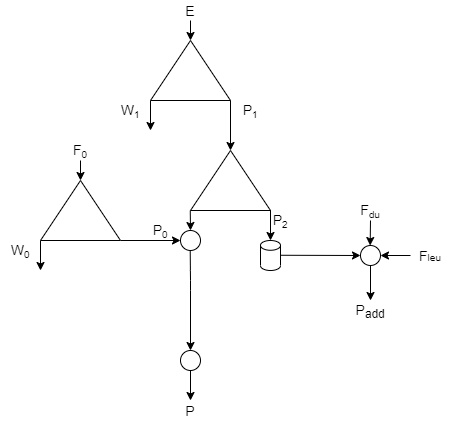
\includegraphics[scale=0.7]{cascades/P2utilization}}
  \caption{Схема независимого вовлечения загрязненной изотопом $^{232}$U фракции с разбавлением обедненным и природным ураном}\label{P2utilization}
\end{figure}

Расчет целевых показателей схемы производился на основе данных составов №1 и №2 (см.постановку задачи), а также предположения двукратного увеличения предела содержания $^{232}$U в продукте, дополнительно производимом из $P_2$ ($1\cdot10^{-6}$\% вместо $5\cdot10^{-7}$\%). Результаты вычислений представлены в таблице \ref{independent}.


\begin{table}[h]
  \centering
  \normalsize\begin{tabulary}{1.0\textwidth}{|C|C|C|C|C|}
    \hline $(C_{232,P})_{lim}$, \% & Цикл № & $P_2$, кг & $\delta(\frac{F_{NU}}{P})$, \% \& $\delta(\frac{\Delta A}{P})$, \% \\\hline 
  $1\cdot10^{-6}$ & 2 & 2,32 &  14,6 \\
   & 5 & 1,96 & 6,3 \\\hline 
   $5\cdot10^{-7}$ & 2 & 2,84 & 7,3 \\
   & 5 & 1,96 & 3,15 \\\hline 
  \end{tabulary}
  \caption{Результаты вовлечения $P_2$ в производство дополнительного НОУ-продукта. Обозначения: $(C_{232,P})_{lim}$ -- предельно допустимая концентрация $^{232}$U в дополнительно производимом на основе $P_2$ продукте. {\label{independent}}}
\end{table}

Значения величин экономии природного урана $\delta(\frac{F_{NU}}{P})$, а также экономии работы разделения $\delta(\frac{\Delta A}{P})$, взятые относительно референтной схемы трехпоточного каскада для обогащения природного урана, тождественны и соответствует доле смеси $P_2$ с ОГФУ в результирующем дополнительно произведенном НОУ-продукте. На эту величину можно заместить эквивалентный по нейтронно-физическим характеристикам НОУ, произведенный на основе природного урана, поэтому эта величина является важнейшим показателем целесообразности применения рассматриваемой схемы утилизации нештатного «отхода», образовавшегося в легком конце второго каскада двухкаскадной схемы. Таким образом, наиболее целесообразно использовать этот способ утилизации нештатного «отхода», образующегося в схеме на начальных рециклах, то есть при меньшей концентрации $^{232}$U, накопившейся в разделяемой смеси. Также  такая схема показывает пропорционально более высокую результативность (двукратно), при более высоких значениях предельно допустимой концентрации результирующего продукта -- $(C_{232,P})_{lim}$.


Значения масс $P_2$ в таблице соответствуют образовавшемуся побочному продукту в процессе производства 1 тонны топлива из регенерата (примерно двух ТВС по $\approx$500 кг). Этот материал, перемешанный с ОГФУ и НОУ-разбавителем в расчитываемом соотношении, в рассмотренной схеме служит поставщиком дополнительного количества $^{235}$U, позволяющего сэкономить сырьевой материал -- природный уран.

Как можно заключить из результатов, представленных в таблице \ref{independent}, предлагаемый способ использования $P_2$ через модификацию схемы двойного каскада с НОУ-разбавителем позволяет экономить дополнительное количество природного урана относительно двойного модифицированного каскада, в котором не предполагается задействование потока легкой фракции второго каскада. А эффект более значителен для случаев, когда задействуется побочный продукт $P_2$ двойного каскада, образующийся на начальных стадиях рециклирования уранового топлива. В рассматриваемом случае -- это второй рецикл (табл. \ref{independent}). Схема рис. \ref{P2utilization} также показывает себя как более предпочтительная в экономии природного урана (вдвое выигрышнее, согласно табл. \ref{independent}), когда предельно допустимая концентрация $^{232}$U в получаемом из $P_2$ конечном продукте допускается в два раза выше ($1\cdot10^{-6}$\% вместо $5\cdot10^{-7}$\%).  Значение экономии природного урана соответствует доле $P_2$, смешанной с обедненным ураном $F_{du}$, до того, как он будет смешан с НОУ-разбавителем $F_{leu}$, полученным из природного урана. Важно заметить, что значение этой доли соответствует экономии работы разделения, которая, в случае отказа от использования $P_2$, была бы затрачена на прямое обогащение природного урана в ординарном каскада для производства аналогичного замещающего количества свежего НОУ-продукта.

Говоря в терминах реакторного топлива, при помощи представленной схемы утилизации, накопленный в ходе производства одной ТВС из регенерата  состава №1 побочный продукт $P_2$ можно использовать для производства дополнительных $\approx$7\%--$\approx$14\% (в зависимости от ограничения на $^{232}$U) свежего НОУ-продукта от дополнительной топливной сборки. Это соответствует возможности произвести дополнительную 15-ю или 8-ю тепловыделяющую сборку (в зависимости от ограничения на $^{232}$U) из накопленного $P_2$, образовавшегося при производстве предыдущих четырнадцати (или семи) ТВС. Таким образом, для современного легководного реактора, такого как, например, российский ВВЭР-1200 или европейский PWR, где активная зона состоит из более чем 150 тепловыделяющих сборок, взяв за основу предложенную схему, можно изготовить дополнительно более 10 ТВС. 



\subsection{Анализ возможности утилизации легкой фракции путем ее перемешивания с обедненным ураном и последующим обогащением}

\subsubsection{Схема составного каскада с НОУ-разбавителем и дополнительным разбавителем потока $P_2$, возвращаемого в цикл}

Другим способом утилизации загрязненной фракции стала многокаскадная схема, представляющая собой модификацию двойного каскада с НОУ-разбавителем, названная <<тройным>> каскадом (рис. \ref{p2_withDepU}) \cite{smirnovApplyingEnrichmentCapacities2018}. Принцип ее работы состоит в следующем.

\begin{figure}[ht]
    \centerfloat{
\includegraphics[scale=0.9]{cascades/p2_withDepU}}
    \caption{Тройной каскад для обогащения регенерированного урана. Обозначения: $E$ -- поток регенерированного урана; $P_1$ -- поток отбора первого каскада, выступающий питанием второго каскада; $P_2$ -- поток отбора второго каскада; $F_{du}$ -- поток ОГФУ-разбавителя, смешиваемого с $P_2$ перед подачей на вход третьего каскада; $W_1$ -- поток отвала первого каскада; $W_2$ -- поток тяжелой фракции (условный «отвал») второго каскада; $P_0$ -- поток НОУ-разбавителя; $P$ -- финальный продукт (товарный низкообогащенный уран (НОУ)), полученный смешиванием потоков $W_2$, $P_0$ и $P_3$, где $P_3$ -- отбор третьего каскада; $W_3$ -- отвал третьего каскада.}\label{p2_withDepU}
\end{figure}

В реализации такой схемы поток легкой фракции второго каскада $P_2$ c концентрацией изотопа $^{235}$U равной 20\% перемешивается со складским ОГФУ и направляется на последующее обогащение в третий каскад (рис. \ref{p2_withDepU}). Отношение, в котором осуществляется смешивание $P_2$ с ОГФУ, определяют исходя из возможности получить НОУ надлежащего качества при обогащении их смеси (оставаясь в рамках ограничений по четным изотопам). Остальные параметры схемы тройного каскада следует подбирать исходя из того, что финальный продукт будет получен смешиванием трех потоков: низкообогащенного <<чистого>> разбавителя $P_0$, тяжелой <<очищенной>> фракции $W_2$ второго каскада и, полученного при обогащении потока $P_2$ и обедненного урана, изотопного состава $P_3$. Управляющими параметрами являются: концентрации на выходах $P_1$ первого и $P_2$ второго каскадов, а также в потоке НОУ-разбавителя $P_0$. При детерминированной их комбинации обеспечивается соответствие предзаданному отношению масс конечного продукта и исходного регенерата, за счет чего выполняется условие полного возврата. При этом проблема высокоактивного отхода решается без выхода за пределы концентрации допустимой для обогащения регенерата (20\%). Также устраняется необходимость обращения с $P_2$, которое в схеме двойного каскада с НОУ-разбавителем с возвратом потока $P_2$ в цикл (рис. \ref{P2utilizationRing}) связано с его отложенным вовлечением из-за зависимости от последующих поступлений на обогащение новых партий (последующих рециклов) регенерата.

Таким образом, решение проблемы накопления нештатного отхода, характерной для двойного каскада с НОУ-разбавителем, состоит в том, что поток легкой фракции второго каскада ($P_2$) перемешивают с обедненным ураном и направляют на последующее обогащение в еще один каскад (крайний правый каскад на рисунке \ref{p2_withDepU}).


Для этого рассмотрим постановку задачи возврата регенерированного урана с последующим замыканием $P_2$, на основе описанной в разделе \ref{triple_descr} каскадной схемы. В качестве разделяемой смеси выбран регенерированный уран, испытавший несколько циклов облучения, а именно состав 2 в таблица \ref{is_compositions_2_5} \cite{smirnovObogashchenieRegenerirovannogoUrana2018}. Требуемая концентрация $^{235}$U в конечном продукте задана равной 4,95\%, коэффициент компенсации реактивности 0,29. Величину коэффициента разделения на единичную разность массовых чисел выбрали равной 1,2. Концентрации $^{235}$U в потоках отвала каскада 1 и каскада для наработки разбавителя задали равной 0,1\%. Ограничение по концентрации $^{232}$U соответствовало $5\cdot10^{-7} \%$, а отношение масс <<исходный регенерат/товарный НОУ>> выбрано равным 0,93 \cite{smirnovObogashchenieRegenerirovannogoUrana2018}.


Анализируя уравнения, описывающие модель <<квазиидеального>> каскада, а также учитывая сформулированную выше постановку задачи, можно прийти к следующим заключениям. При заданных внешних условиях и требованиях к составу товарного НОУ, такая каскадная схема имеет 6 неизвестных переменные: 1) концентрация $^{235}$U в потоке $P_{1}$; 2) концентрация $^{235}$U в потоке $P_{2}$; 3) концентрация $^{235}$U в потоке $W_{2}$; 4) концентрация $^{235}$U в потоке НОУ-разбавителя $P_{0}$; 5) $^{235}$U в потоке $W_{3}$ ; 6) Доля $P_2$ в питании третьего каскада. При этом эти параметры явно и неявно связаны двумя уравнениями, получаемыми для невязок по заданным концентрациям изотопов $^{232}$U и $^{235}$U:

\begin{enumerate}
    \item $\delta_{1}=C_{235,P\textit{ экв.}}-(C_{235,P\textit{ NU}}+\Delta C_{235})$ -- невязка по концентрации $^{235}$U в конечном НОУ-продукте, с учетом поправки на присутствие изотопа $^{236}$U. Величина $\delta_{1}$ фактически определяет точность достижения условия компенсации $^{236}$U;
    \item $\delta_{2}=C_{232,P\textit{ расч.}}-C_{232,P\textit{ треб.}}$ -- разница между рассчитанным значением концентрации $^{232}$U в конечном НОУ-продукте и заданным ограничением для концентрации этого изотопа.
\end{enumerate}

Таким образом, для нахождения 6 переменных имеем 2 уравнения. Это означает, что 4 переменные задачи можно рассматривать в качестве варьируемых параметров. В качестве них будем рассматривать концентрации $^{235}$U в потоках $P_{1}$, $P_{2}$ и $W_{3}$, а также долю $P_2$ в питании третьего каскада. Из приведенных рассуждений следует, что достижение требуемых внешних условий возможно при формально бесконечном множестве наборов концентраций в отборе первого и второго каскадов. Для того, чтобы выбрать из этого набора какой-то из вариантов необходимо проведение оптимизационного расчёта с использованием некоторого критерия эффективности.

Таким образом, цель решения оптимизационной задачи: при заданных внешних условиях и выполнении заданных ограничений на концентрации чётных изотопов в потоке продукта, а также выполнении условия полного использования регенерата, определить наилучшее значение критерия эффективности, в зависимости от следующих управляющих оптимизационных переменных: концентрации $^{235}$U в потоках $P_1$, $P_2$ и $W_3$ и отношение потоков $F_{du}$/$P_2$.


Также, помимо минимума расхода работы разделения, оптимизационным критерием может выступать минимизация расхода природного урана, а также максимум суммарной степени извлечения $^{235}$U в схеме \ref{Rec3} и из регенерата \ref{RecR3} для тройного каскада, где $E$ -- это поток регенерата, а $DepU_{3}$ -- поток разбавляющего $P_2$ ОГФУ.

\begin{equation} \label{Rec3} 
    Y_{f} = \frac{LEU Product \cdot C_np}{F_0 \cdot C_{NU}^{235} + E \cdot C_{E}^{235} + {DepU}_3 \cdot C_{DepU}^{235}},
\end{equation} 
\begin{equation} \label{RecR3} 
    Y_{E} = \frac{W_2\cdot C_{W_2}^{235}+P_3\cdot C_{P_3}^{235}\cdot \frac{P_2\cdot C_{P_2}^{235}}{P_2\cdot C_{P_2}^{235}+ {DepU}_3 \cdot C_{DepU}^{235}}}{E \cdot C_{E}^{235}}        
\end{equation} 

Такой тип оптимизационной задачи также как и для предыдущих составных схем представляет собой задачу условной оптимизации функции многих переменных. В диссертационной работе предложена оригинальная методика, основанная на использовании современных методов условной оптимизации и реализованная в виде разработанного программного кода.
Следует отметить, что в литературе по данной тематике отсутствуют методики оптимизации трех- и четырехкаскадных схем в случае разделения многокомпонентных смесей. Фактически подобные задачи решены впервые.

Рассмотрим предложенный в данной работе алгоритм подбора параметров каскадной схемы, который позволяет осуществить расчет двойного каскада с НОУ-разбавителем.

\begin{enumerate}
    \item задание начальных условий и требований к конечному продукту -- товарному НОУ;
    \item задание диапазона варьирования переменных оптимизации;    
    \item задание начальных приближений для оптимизационных переменных -- концентраций $^{235}$U в потоках $P_1$ и $P_2$;
    \item для заданных значений концентраций $^{235}$U в потоках $P_1$ и $P_2$ осуществляют решение системы нелинейных алгебраических уравнений для невязок по заданным концентрациям изотопов $^{232}$U и $^{235}$U в товарном НОУ, а искомыми из решения системы переменными выступают концентрации $^{235}$U в потоке отвала второго каскада и в потоке отбора каскада, нарабатывающего НОУ-разбавитель. В рамках работы для решения СНАУ использовали вычислительный пакет MINPACK \cite{moreMINPACK}, использующий квазиньютоновский численный алгоритм <<trust-region>>, для которого якобиан матрицы системы вычисляют методом автодифференциации.
        \begin{itemize}
        \item для каждой итерации решателя СНАУ, выполняется оптимизационный алгоритм поиска глобального оптимума для заданного критерия эффективности, с помощью которого подбираются такие параметры схемы как: доля потока $P_2$ в питании третьего каскада; концентрации $^{235}$U в потоке отвала третьего каскада в интервалах [0.00001, 0.5] и [0.08\%, 0.13\%] соответственно. Для этого используется алгоритм оптимизации SHGO (simplicial homology global optimization) вычислительного пакета SciPy для Python  \cite{virtanenSciPyFundamentalAlgorithms2020a}.
        
        \item Внутри итерационной процедуры решения системы уравнений для текущий значений искомых переменных проводят расчёт основных параметров входящих в схему одиночных ординарных каскадов. Для этого также используют методы численного решения систем нелинейных алгебраических уравнений, возникающих для невязок по заданным концентрациям $^{235}$U в выходящих потоках каскадов. Из решения таких СНАУ определяют длины секций каждого из каскадов, что далее позволяет рассчитать их остальные параметры и определить доли потоков $W_2$, $P_3$  и $P_0$ в конечном продукте, для того чтобы рассчитать текущие концентрации всех компонентов в товарном НОУ. Для этого, на основе вычисленных отношений потоков $\frac{P_{1}}{E}$, $\frac{W_{2}}{P_{1}}$ и $\frac{P_{3}}{F_{3}}$ для первого, второго и третьего каскадов, а также заданного условиями задачи отношения $\frac{E}{P}$, где $E$ -- это поток регенерата, а $P$ -- поток финального НОУ-продукта, вычисляют значение $\frac{W_{2}}{P}$ как произведение $\frac{P_{1}}{E}$, $\frac{W_{2}}{P_{1}}$ и $\frac{E}{P}$. Затем, вычитанием из единицы отношения $\frac{W_{2}}{P}$, получают $\frac{P_{0}}{P}$.
        
        \item поочередно складывая покомпонентно умноженные доли $\frac{W_{2}}{P}$, $\frac{P_{3}}{P}$ и $\frac{P_{0}}{P}$ на соответствующие изотопные концентрации потоков $W_2$, $P_3$ и $P_0$, получается массив изотопных концентраций конечного НОУ-продукта
        \end{itemize}
    После выполнения всех этих процедур рассчитывают текущие величины расхождения по заданным концентрациям изотопов $^{232}$U и $^{235}$U в товарном НОУ. В рамках выполненных расчётов для каждой из невязок относительная ошибка (отклонение от единицы отношений левой и правой частей равенства) не должна была превысить величину $10^{-8}$;
    \item соответствие выполненных условий для невязок означает сходимость численного метода -- завершение итерационной процедуры решения СНАУ и сохранение полученной величины критерия эффективности при заданных значениях концентраций $^{235}$U в потоках $P_1$ и $P_2$;
    \item повтор п. 3-5 до тех пор пока не будут выполнены условия выхода из оптимизационной процедуры, в данном случае допустимая относительная ошибка (relevant tolerance) не будет превышать значения $10^{-8}$;
    \item выбор наилучшей величины критерия эффективности и расчёт параметров оптимального варианта каскадной схемы.
\end{enumerate}




Для анализа возможностей схемы тройного каскада с НОУ-разбавителем, представим расчет, оценивающий издержки ее применения для возврата регенерата состава №2. 
В качестве ключевых оцениваемых характеристик будем опираться на интегральные характеристики:
\begin{enumerate}
    \item $\delta(\frac{\Delta A}{P})$ -- экономия работы разделения относительно референтной схемы трехпоточного каскада для обогащения природного урана (см. Приложение). Наибольшая экономия соответствует минимуму суммарного потока схемы \ref{GrindEQ__1_73_}. Если величина отрицательная, абсолютное значение соответствует потерям работы разделения, по сравнению с референтной схемы трехпоточного каскада для обогащения природного урана;
    \item $\delta(\frac{F_{NU}}{P})$ -- экономия природного урана относительно референтной схемы трехпоточного каскада для обогащения природного урана.  Наибольшая экономия соответствует минимуму удельного расхода природного урана схемы. Если величина отрицательна, абсолютное значение соответствует перерасходу природного урана, по сравнению с референтной схемы трехпоточного каскада для обогащения природного урана.
\end{enumerate}

Проведем сравнение со схемой с разбавлением регенерата природным ураном перед подачей в ординарный трехпоточный каскад \ref{o3} \cite{smirnovMethodEnrichReprocessed2019}. Результаты расчетов представлены в таблицах \ref{tr_ch} и \ref{tr_prodF}, где показаны изотопный состав НОУ коммерческого уровня и массовые потоки, отнесенные к 1 тонне продукта, полученного в предлагаемом тройном каскаде, соответственно.

\begin{table}[h]
\centering
\normalsize\begin{tabulary}{1.0\textwidth}{|C|C|C|C|C|C|C|}
    \hline
    \diagbox{Каскад}{Параметр} & $\delta(\frac{F_{NU}}{P})$, \% & $\delta(\frac{\Delta A}{P})$, \% & $\frac{E}{P}$ \\\hline
    % Ординарный модифицированный & 7,1 & -3,6 & 0,49 \\\hline
    Тройной каскад & 38,3 & -97,3 &  0,93 \\\hline
\end{tabulary}
\caption{{Оцениваемые параметры рассматриваемых схем{\label{tr_ch}}}}
\end{table}

Обе сравниваемые схемы должны обеспечить производство НОУ коммерческого качества, однако только тройной каскад позволяет расходовать требуемое отношение регенерата к единице продукта.


\begin{table}[h]
    \centering
    \normalsize
    \begin{tabulary}{1.0\textwidth}{|c|c|c|c|c|c|}
        \hline Массовое число & 232 & 233 & 234 & 235 & 236\\
        \hline C, \% & $5\cdot10^{-7}$ & $6,88\cdot10^{-7}$ & $5,31\cdot10^{-2}$ & $5,11$ & $5,72\cdot10^{-1}$ \\\hline
    \end{tabulary}
\caption{{Изотопный состав НОУ-продукта схемы тройного каскада.{\label{tr_prod}}}}
\end{table}

\begin{table}[h]
    \centering
    \addtolength{\tabcolsep}{-5pt}
    \begin{tabulary}{1.0\textwidth}{|c|c|c|c|c|c|c|c|c|c|c|c|c|}
        \hline поток & $P$ & $E$ & $W_1$ & $P_1$ & $W_2$ & $P_2$ & $F_{du}$ & $W_3$ & $P_0$ & $P_3$ & $F_0$ & $W_0$\\
        \hline m, кг & $1\cdot10^{3}$ & 930 & 833 & 96,6 & 80,9 & 15,8 & $1,571\cdot10^{5}$ & $1,568\cdot10^{5}$ & 628,5 & 290,5 & $4,9\cdot10^{3}$ & $4,3\cdot10^{3}$\\
        % \hline C, \% & $5\cdot10^{-7}$ & $1,03\cdot10^{-6}$ & 0,1 & 9,41 & 7,34 & 20 & 0,1 & 0,093 & 4,9 & - & 0,71 & 0,1\\
        \hline
\end{tabulary}
\caption{{Массовые потоки в схеме тройного каскада.{\label{tr_prodF}}}}
\end{table}


Эти результаты показывают, что предложенная схема решает поставленную задачу. Даже при выбранном «грязном» составе регенерированного урана -- составе №2 -- можно сэкономить более трети природного урана  по сравнению с референтной схемой ординарного каскада. Однако, такие преимущества влекут за собой увеличение затрат разделительной работы, а следовательно, и количества центрифуг по сравнению с ординарным трехпоточным каскадом, который обогащает природный уран ($\approx$97\%). Схема также позволяет производить НОУ товарного качества, расходуя заранее определенное количество переработанного урана без нежелательных нештатных побочных продуктов, за исключением т.н. хвостов разделительного производства (потоков отходов) разделительных каскадов в виде обедненного урана в потоках $W_0$, $W_1$ $W_3$.

В результате своей работы схема производит $\approx$162 тонны обедненного урана. При этом схема потребляет $\approx$157 тонн складских запасов обедненного урана. Следовательно, фактический выход обедненного урана составляет $\approx$4,76 тонн, при том что ординарный каскад для обогащения природного урана при производстве такого же количества продукта (1 тонна) производит $\approx$7 тонн, то есть схема тройного каскада с НОУ-разбавителем и дополнительным разбавителем потока $P_2$, возвращаемого в цикл позволяет в полтора раза уменьшить накопление ОГФУ.


Как было показано в работе \cite{gusevMultycascadeEnrichmentSchemes2020}, для схемы тройного каскада возможно регулировать расход природного урана и работы разделения. Например, ценой расхода дополнительных $\approx$25\% работы разделения, удается вернуть заданное количество переработанного урана, прошедшего пятикратное (5 топливных кампаний) облучение, сэкономив $\approx$15\% природного урана, при этом вовлекая в производство единицы конечного продукта $\approx$31 единицы смеси обедненного урана. Для экономии же природного урана достигающей $\approx$23\%, необходимо, использовав $\approx$74,5 единиц ОГФУ на единицу продукта, допустив перерасход работы разделения на  уровне $\approx$50\%. Показатели приведены в соотношении с аналогичными для схемы ординарного каскада для обогащения природного урана, получающего на выходах в продукте и отвале такие же концентрации $^{235}$U (соответствующую $(C_{235,P})_\textit{экв.}$ в продукте).










Как результат, схема тройного каскада с НОУ-разбавителем и дополнительным разбавителем потока $P_2$, возвращаемого в цикл, позволяя в полноте решить поставленную задачу, не оставляет никакого нештатного отхода, требующего особых мер обращения. В конечном итоге образуется только штатный отход в виде отвалов $W_1$ и $W_3$ , процедуры обращения с которыми на разделительном производстве технологически отработаны. Если получить их смешением ($W_1$ и $W_3$) обедненный уран, он будет содержать изотопы $^{232,234}$U в количествах в десятки/сотни раз сниженных, относительно исходного регенерата. Следовательно, полученный в такой схеме обедненный уран может быть переведен в двуокись урана, например, при помощи установки «W-ЭХЗ». Отсутствие нештатных отходов, загрязненных четными изотопами и является отличительным достоинством рассмотренной схемы, тогда как недостатком выступают дополнительные потери работы разделения, возникающие при перемешивании потока $P_2$ и подмешиваемого к нему в качестве разбавителя ОГФУ.


В качестве итогового списка характеристических особенностей схемы тройного каскада следует обозначить следующие:

\begin{enumerate}
    \item применима для обогащения регенерированного урана в условиях многократного рецикла и позволяет получать продукт, отвечающий всем требованиям по концентрациям четных изотопов для регенерата различного исходного состава как показано на рассматриваемых входных изотопных составах;
    \item достоинством схемы является полное отсутствие нештатных отходов, требующих специального обращения, поскольку на выходе из схемы, помимо основного продукта, возникают только потоки обедненного урана в виде отвалов каскадов схемы. Причем, в отличие от схемы двойного каскада с НОУ-разбавителем, отход отсутствует при любом варианте использования: как для однократного обогащения регенерированного урана, так и в условиях постоянных поступлений партий регенерированного урана последовательных перегрузок реактора;
    \item как и предшествующие схемы, схема позволяет задействовать для воспроизводства ядерного топлива накопленный в значительных количествах обедненный уран;
    \item в схеме отделены участки обогащения регенерированного урана и участок обогащения обедненного или природного урана (каскад, расположенный на схеме слева (рис. 
    \ref{p2_withDepU})), не загрязненного четными изотопами. В дальнейшем это позволит использовать оборудование этого каскада для обогащения природного урана или другого сырьевого материала, не загрязненного четными изотопами;
    % \item получаемый в схеме отвал регенерированного урана в потока $W_1$ и $W_3$ имеет содержание изотопа $^{232}$U ниже, чем исходный регенерат. Подобный материал можно длительно хранить или отправить на переработку в установке дефторирования. В случае же необходимости дополнительного понижения концентраций четных изотопов данный поток может быть дополнительно разбавлен конечными отвалами с обогащением ниже 0,13\%. 
    \item недостатком схемы являются потери работы разделения из-за необходимости:
    \begin{enumerate}
        \item обеднять отбор первого каскада в последующем втором каскаде;
        \item смешивание потоков $W_2$ с НОУ-разбавителем $P_0$, а затем и с $P_3$ в которых различается содержание изотопа $^{235}$U;
        \item смешивания потоков $P_2$ и $F_{du}$ на входе в третий каскад.
    \end{enumerate}
\end{enumerate}


Слабое изменение параметров каскадной схемы в условиях многократного рецикла позволяет говорить о возможности «настройки» данной каскадной схемы на возможность работы с регенератом различных рециклов при минимальных изменениях параметров. В частности, для данной схемы возможно подобрать «унифицированный» разбавитель с фиксированным содержанием 235U, что могло бы позволить не привязывать напрямую мощности по получению разбавителя из обедненного урана (каскад 3) к каскадам, работающим с регенератом. Иными словами, в этом случае разбавитель мог бы нарабатываться независимо от поступлений конкретных партий регенерата.



В качестве выводов, относящихся ко всем рассмотренным схемам, приведем следующие:
\begin{enumerate}
    \item схемы на основе двойного каскада, использующие НОУ-разбавитель, принципиально пригодны для решения задачи обогащения регенерированного урана в рамках многократного рецикла урановой составляющей топлива легководных реакторов. При этом каждая из схем имеет собственные достоинства и недостатки;
    \item характерным недостатком схемы, не предполагающей утилизацию нештатного отхода, образующегося в потоке $P_2$, является проблема с обращением с этим материалом, с высоким содержанием как четных изотопов (на 1-2 порядка выше, чем пределы для товарного НОУ) и $^{235}$U (до 20\% или, в некоторых случаях, до 90\%, в зависимости от выбранного режима работы каскадной схемы). Одним из вариантов обращения с ним, помимо схемы независимой утилизации побочного продукта легкой фракции второго каскада схемы двойного каскада с НОУ-разбавителем (рис. \ref{P2utilization}), может стать его перемешивание с отвалом первого каскада при обогащении регенерата. Оценки показали, что в этом случае возможно получить обедненный уран с приемлемым содержанием $^{232}$U (не выше $5\cdot10^{-7}$\%);
    \item характерными недостатком схемы двойного каскада с НОУ-разбавителем с возвратом потока $P_2$ в цикл (рис. \ref{P2utilizationRing}) является возврат значительной части четных изотопов на вход каскадной схемы;
    \item характерным недостатком схемы тройного каскада (рис. \ref{p2_withDepU}) являются дополнительные затраты работы разделения по отношению к схемам двойного каскада с НОУ-разбавителем, возникающие при обогащении разбавленного обедненным ураном отхода второго каскада схемы, загрязненного четными изотопами.
  \end{enumerate}

Анализ эффективности предложенных каскадных схем с точки зрения потерь $^{235}$U показал, что перспективными вариантами для дальнейшей технико-экономической проработки являются каскадные схемы двойного каскада с НОУ-разбавителем (рис. \ref{p2left}) и тройного каскада (рис. \ref{p2_withDepU}). Cхема двойного каскада с НОУ-разбавителем на каждом из рассмотренных рециклах позволяет извлечь более 80\% от массы $^{235}$U из исходного регенерированного урана, поступившего на обогащение.


Для выбора конкретного варианта каскадной схемы для организации производственного процесса, необходим детальный технико-экономический анализ каждой из схем на основе их интегральных показателей, таких как расход сырьевых материалов и работы разделения, в контексте всей цепочки ядерного топливного цикла, а также с учетом возникающих в этой цепочке изменений при использовании регенерата урана по отношению к открытому топливному циклу. Помимо этого, необходима проработка технологических проблем каждой из схем, в частности, с точки зрения возможности эксплуатации и обслуживания оборудования в условиях работы с материалами, имеющими более высокую, чем природный уран удельную активность. Например, подобные условия возникают в каскадах, концентрирующих в легкой фракции $\alpha$-активные изотопы $^{232,234}$U.

\clearpage

